\begin{ESKDtitlePage}
  \begin{flushright}
    \textbf{ПРИЛОЖЕНИЕ Г} \enspace\enspace
  \end{flushright}
  
  \begin{center}
    % \envDiplomMinistr \\
    \envDiplomEducation \\
    \envDiplomUniversity \\
    \envDiplomCathedra \\
  \end{center}

  \vfill

  \begin{center}
    \textbf{ИНСТРУКЦИЯ ПО УСТАНОВКЕ ПО}
  \end{center}

  \vfill

  \begin{center}
    \envCode \\
  \end{center}

  \vfill

  \begin{flushright}
  \begin{minipage}[t]{.49\textwidth}
    \begin{minipage}[t]{.75\textwidth}
      \begin{flushright}
        \envDiplomTeacherInfo\\
        \hspace{0pt}\\
        \envDiplomStudentInfo\\
        \hspace{0pt}\\
        Консультанты:\\
        \envDiplomEspdInfo\\
        \hspace{0pt}\\
        \envDiplomRecendentInfo\\
      \end{flushright}
    \end{minipage}
  \end{minipage}
  \begin{minipage}[t]{.49\textwidth}
    \begin{flushright}
      \begin{minipage}[t]{.75\textwidth}
        \envDiplomTeacherInitials~\envDiplomTeacherSurname\\ % Руководитель
        \hspace{0pt}\\
        \envDiplomStudentInitials~\envDiplomStudentSurname\\ % Выполнил
        \hspace{0pt}\\
        \hspace{0pt}\\ % Консультанты:
        \envDiplomEspdInitials~\envDiplomEspdSurname\\ % по ЕСПД
        \hspace{0pt}\\
        \envDiplomRecendentInitials~\envDiplomRecendentSurname\\ % рецензент
      \end{minipage}
    \end{flushright}
  \end{minipage}
\end{flushright}


  \vfill

  \begin{center}
    \ESKDtheYear
  \end{center}
\end{ESKDtitlePage}


\newpage
\section*{АННОТАЦИЯ}
\ESKDthisStyle{empty}

% \pageref{LastPage}~c., \totalfigures~рис., \totaltables~табл.
% \ESKDtotal{page}~с., \ESKDtotal{figure}~рис., \ESKDtotal{table}~табл., \ESKDtotal{bibitem}
\pageref{LastPage}~c./65~с.,
\totalfigures~рис.,
\totaltables~табл.,
\ESKDtotal{bibitem}~ист.~лит.,
1 прил.,
6 л. граф. матер.

\hspace{0pt}

Данный дипломный проект посвящен проектированию БД (MySQL),
которая хранит данные
о зарегистрированых пользователях (юридических лиц),
брендах, категориях, номенклатуре, галереи картинок, характеристиках товаров,
новостях, контактов фирмы, о оформленных заказах.
Дипломный проект посвящен реализации серверной части на базе NestTS на языке программирования TypeScript,
с документацией Swagger UI,
посвящен реализации мобильного приложения на базе React Native на языке программирования TypeScript
и веб-сайта с панелью администратора и менеджера на базе Create-React-App на языке программирования TypeScript.

Дипломный проект включает в себя такие разделы как
анализ предметной области,
проектирование системы,
реализация и испытание системы,
расчет экономических показателей.

% \vfill
\hspace{0pt}

\hspace{0pt}

\begin{tabular}{p{3.2cm}p{12cm}}
    Составитель:
    & \envDiplomStudentSurname~\envDiplomStudentInitials,
    студент группы ПО-4,
    факультета электронно информационных систем,
    спецальности <<Программное обеспечение информационных технологий>> (1-40 01 01),
    учереждения образования <<Брестский государственный технический университет>>
    \\

    \envDiplomRecendentInfo:
    & \envDiplomRecendentSurname~\envDiplomRecendentInitials,
    заведующий кафедры высшей математики,
    кандидат технических наук,
    доцент,
    учереждения образования <<Брестский государственный технический университет>>
\end{tabular}

% \vfill

\hspace{0pt}

\hspace{0pt}

Учереждение образования
    
<<Брестский государственный технический университет>>, \ESKDtheYear


\newpage
\ESKDthisStyle{formII}
\tableofcontents
\hspace{0pt}\\
ПРИЛОЖЕНИЕ А. Техническое задание \\
ПРИЛОЖЕНИЕ Б. Набор тестовых задания для проверки БД \\
ПРИЛОЖЕНИЕ В. Результаты загрузки и проверки БД \\
ПРИЛОЖЕНИЕ Г. Инструкция по установке ПО \\
ПРИЛОЖЕНИЕ Д. Текст программы \\

\newpage
\phantomsection
\addcontentsline{toc}{section}{ВВЕДЕНИЕ}
\section*{ВВЕДЕНИЕ}
% Цели-задачи-метод-результаты

В настоящее время разработка мобильных приложений стала неотъемлемой частью современной технологической среды,
предоставляющей уникальные возможности и решения в различных областях жизни.
С мобильными приложениями мы можем создавать инновационные продукты, улучшать коммуникацию,
повышать эффективность работы и сделать нашу жизнь более удобной и комфортной.

Благодаря мобильным приложениям мы можем осуществлять заказы и покупки онлайн,
получать доступ к информации и услугам в любое время и в любом месте.
Они стали незаменимыми инструментами в сфере электронной коммерции, финансовых услуг,
медицины, образования, развлечений и других отраслях. Мобильные приложения стали платформой для инноваций и новых идей,
способствуя развитию экономики и повышению качества жизни.

Целью дипломного проектирования является готовая база данных и мобильное приложение
для учета заказов юридических лиц.

% В рамках дипломного проектирования объектом является разработка мобильного приложения.
% Объектом дипломного проектирования является система учета заказов для юридических лиц.
Объектом иследования является система учета заказов.
Предметом - оптимизация процесса заказа товаров для юридических лиц
через разработанное мобильное приложение.

Задачами данного дипломного проектирования является обследование объекта автоматизации.

Проектирование базы данных и реализация мобильного приложения ведётся следующими методами:
описываем программу в виде UML диграмы предецентов, диграмы последовательности, диграмы развертывания;
описываем базу данных в виде логической модели в draw.io;
описываем таблицы базы данных в виде класcов на языке программирования TypeScript;
реализуем Rest API приложение на фреймворке NestJS на языке TypeScript;
документируем HTTP запросы с помощью Swagger UI;
реализуем мобильное приложение с помощью библиотеки React Native на языке TypeScript.

Результатом дипломного проектирования является мобильное приложение и готовая база данных,
которая хранит данные о брендах, категориях, номенклатуре,
хакрактеиристиках номенклатуры,
списка картинок номенклатуры,
данных юридических лиц,
данных о заказе и его статусе.

В рамках дипломного проектирования представлен комплексный подход,
включающий:
проектирование базы данных;
разработку серверной части (backend) для обеспечения Rest API приложения;
разработку веб-сайта с панелью администратора (frontend), предназначенной для редактирования брендов, категорий и номенклатуры;
разработку веб-сайта с панелью менеджера (frontend), обеспечивающий просмотр заказов из базы данных;
создание мобильного приложения (frontend),
которое позволяет осуществлять заказ номенклатуры.

В первом разделе
проводим анализ существующих мобильных приложений таких как
WildBerries, OZ.by, LC Waikiki, Lamoda, De Facto, Ali Express;
выбираем базу данных, средства для реализации серверной части (backend) и мобильного приложения (frontend).

Во втором разделе
описываем приложение UML диграмой прецедентов.
Работа приложения показазываем на UML диаграмме развертывания.
В этом разделе описываем логическую модель и переводим ее в физическую модель используя миграции TypeORM.

В третьем разделе
представлена документация SwaggerUI, которая играет важную роль в тестировании эндпоинтов.
SwaggerUI предоставляет удобный интерфейс для взаимодействия с эндпоинтами системы,
позволяя разработчикам и тестировщикам отправлять запросы на серверную часть (backend)
и получать соответствующие ответы.
Кроме того, в третьем разделе приведены скриншоты мобильного приложения,
которые позволяют ознакомиться с его внешним видом и пользовательским интерфейсом.
Эти изображения предоставляют визуальное представление о функциональности и возможностях приложения,
позволяя получить наглядное представление о его работе.

В четвёртом разделе
производится сравнение объема функций из каталога с уточненным объемом функций разрабатываемого проекта.
Осуществляется расчет себестоимости оборудования по различным статьям,
включая отчисления на социальные нужды, материалы и комплектующие,
машинное время, накладные расходы, а также затраты на освоение и сопровождение программного средства.
Также производится расчет плановой прибыли, прогнозируемой цены без налогов, отпускной цены и
расчета прибыли от реализации программного обеспечения за вычетом налога на прибыль.

% В приложении А
% представлено техническое задание, которое поможет лучше понять требования к проекту.

% В приложении Б
% представлены данные для проверки базы данных, что позволяет убедиться в корректности ее работы.

% В приложении В
% можно ознакомиться с результатами загрузки данных в базу данных.

% В приложении Г
% представлена инструкция по установке необходимого программного обеспечения для успешной настройки и запуска проекта.
% Инструкция включает установку NodeJS, установку пакетного менеджера yarn,
% а также установку Docker для запуска БД на операционной системе Windows 10.
% % Эти инструменты необходимы для работы с серверной частью (backend), разработанной на NestTS,
% % мобильного приложения (frontend), написанного на React Native с использованием TypeScript,
% % а также веб-сайтом с панелью администратора (frontend), разработанным с использованием NextTS.
% % Эта инструкция обеспечит удобство и понятность при настройке необходимого программного обеспечения,
% % что позволит пользователям успешно разрабатывать и демонстрировать проект.

% В приложении Д приведен каталогом API,
% где можно ознакомится со списком картинок с их путями (URL) и HTTP методами офромленными в SwaggerUI.

% В приложении E
% прикреплен диск, содержащий исходные коды серверной части, базы данных,
% мобильного приложения, веб-приложения с панелью администратора и менеджера,
% а также отчет, оформленный в LaTeX.

В приложении А
прикреплен диск, содержащий исходные коды серверной части, базы данных,
мобильного приложения, веб-приложения с панелью администратора и менеджера,
а также отчет, оформленный в LaTeX.

\newpage


\section{АНАЛИЗ ПРЕДМЕТНОЙ ОБЛАСТИ}
\subsection{Обзор существующих решений}

\textbf{Анализ мобильных приложений} проводится для того, чтобы выявить основные функциональные возможности, структуру и дизайн.
Для этого возьмем нескольких популярных мобильных приложений, включая
Wildberries \cite{AndroidWildberries},
OZ.by~\cite{AndroidOzBy},
LC Waikiki \cite{AndroidLcWaikiki},
Lamoda \cite{AndroidLamoda},
DeFacto \cite{AndroidDefacto}
и AliExpress \cite{AndroidAliExpress}.

Для анализа будут сделаны скриншоты главного экрана, экрана категорий, корзины, избранных, страницы с товаром, вид характеристик товара и входа в аккаунт
для каждого приложения.

Из анализа стало ясно, что у каждого приложения есть свои сильные и слабые стороны.
В целом, анализ мобильных приложений позволяет выявить недостатки и возможности для улучшения существующих приложений.

\textbf{Главный экран} в мобильном приложении по заказу товаров является первым взаимодействием пользователя с приложением.
Он должен быть удобным и информативным, чтобы привлечь внимание пользователя и помочь ему быстро найти нужный товар.
На главном экране обычно отображается список категорий товаров, актуальные предложения, новые поступления и лучшие продажи.
Также на главном экране может быть размещена поисковая строка, чтобы пользователь мог быстро найти интересующий его товар.
Важно, чтобы главный экран был интуитивно понятен и легко навигировался, чтобы пользователь мог быстро и легко перейти к нужному разделу приложения.

Скриншоты главного экрана приведены на рис.~\ref{fig:analyzHome}.

\textbf{Экран с номенклатурой} в мобильном приложении - это страница, на которой пользователь может просмотреть полную информацию о товаре,
включая его название, описание, изображения, цену и характеристики.

Скриншоты экрана с товаром приведены на рис.~\ref{fig:analyzItem}.

С другой стороны, \textbf{экран с номенклатурой} в мобильном приложении по заказу товаров - это страница,
на которой отображается список доступных для покупки товаров с их характеристиками,
ценами и возможностью добавления в корзину.
Покупателю нужно знать характеристики товаров,
чтобы сравнить и выбрать наиболее подходящий для своих нужд.
Это может включать в себя такие параметры, как размер, цвет, материал, вес и другие особенности товара.

Скриншоты экрана с характеристиками приведены на рис.~\ref{fig:analyzItemCharacteristic}.

\textbf{Экран с корзиной номенклатуры} - это функциональность в мобильном приложении,
которая позволяет покупателю собирать товары, которые он хочет купить.
Покупатель может добавлять и удалять товары из корзины, изменять количество товаров,
просматривать общую стоимость и оформлять заказ.

Показ корзины без регистрации важен,
так как многие покупатели не желают тратить время на регистрацию в приложении,
прежде чем начать совершать покупки.
Показ корзины без регистрации также дает покупателям возможность быстро и легко просматривать товары,
которые они добавили в корзину, и оценивать общую стоимость заказа, прежде чем оформлять покупку.

Скриншоты экрана с корзиной приведены на рис.~\ref{fig:analyzBasket}.

\textbf{Экран авторизации} - это страница, на которой пользователь вводит свои данные для входа
в приложение или сайт.
Это может включать в себя поле для ввода электронной почты или логина, 
 также поле для ввода пароля.
Экран авторизации может также включать в себя функции восстановления пароля
или регистрации нового пользователя. 

Скриншоты экрана авторизации приведены на рис.~\ref{fig:analyzLogin}.

\textbf{Экран с избранным} в мобильном приложении представляет собой список товаров,
которые пользователь отметил для последующего просмотра или покупки.
Он предназначен для того, чтобы пользователь мог сохранить товары, которые ему интересны,
но которые он не хочет покупать сразу.

Избранные товары должны быть доступны только авторизованным пользователям,
так как это позволяет сохранять выбранные товары на протяжении нескольких сессий
и переносить их на другие устройства.
Также это предотвращает потерю списка избранного при случайном выходе из приложения
или при сбое в работе устройства.
В отличие от корзины, которая представляет собой список товаров, находящихся в процессе покупки,
избранные товары не требуют немедленной покупки,
а могут быть отложены на неопределенное время.

Когда пользователь не авторизован, нажатие на кнопку сердечко приводит к появлению экрана авторизации.
После того, как пользователь войдет в свой аккаунт,
он может вернуться на страницу товара и добавить его в избранное.
Если пользователь еще не зарегистрирован,
то после нажатия на кнопку сердечко ему будет предложено зарегистрироваться и создать аккаунт.

Скриншоты экрана избранных приведены на рис.~\ref{fig:analyzLike}.

\begin{figure}[!p]
  \centering

  \begin{minipage}{0.16\textwidth}
    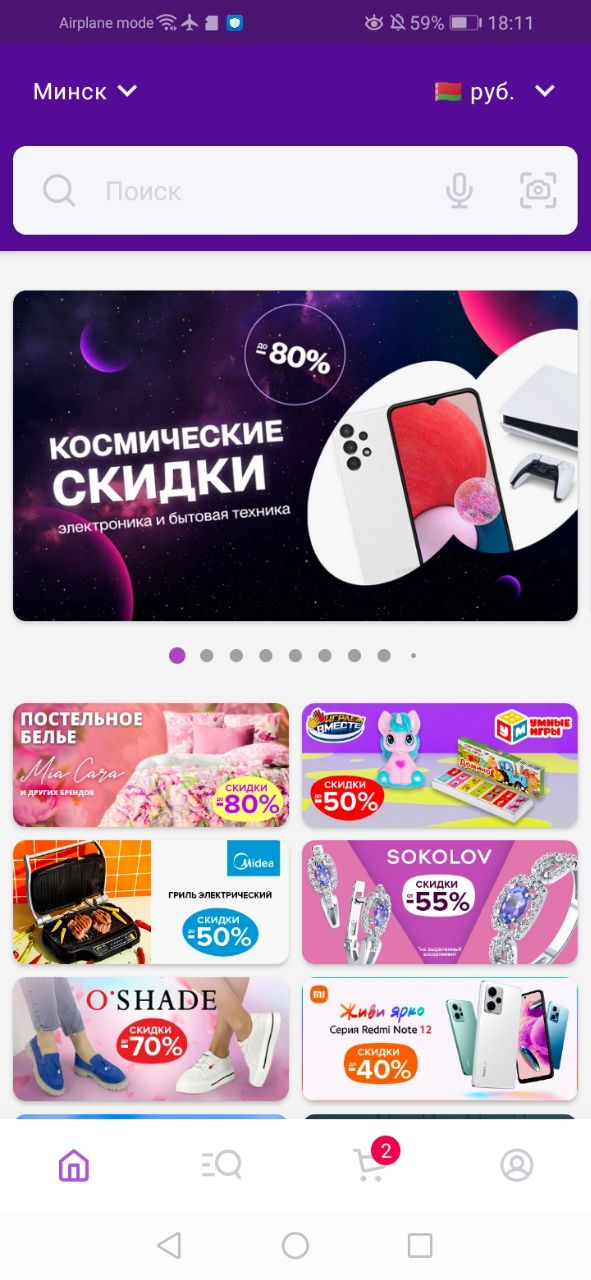
\includegraphics[width=.99\linewidth]
    {images/candidates/Wildberies/Home.jpg}
  \end{minipage}
  \begin{minipage}{0.16\textwidth}
    
\includegraphics[width=.99\linewidth]
    {images/candidates/OZby/Home.jpg}
  \end{minipage}
  \begin{minipage}{0.16\textwidth}
    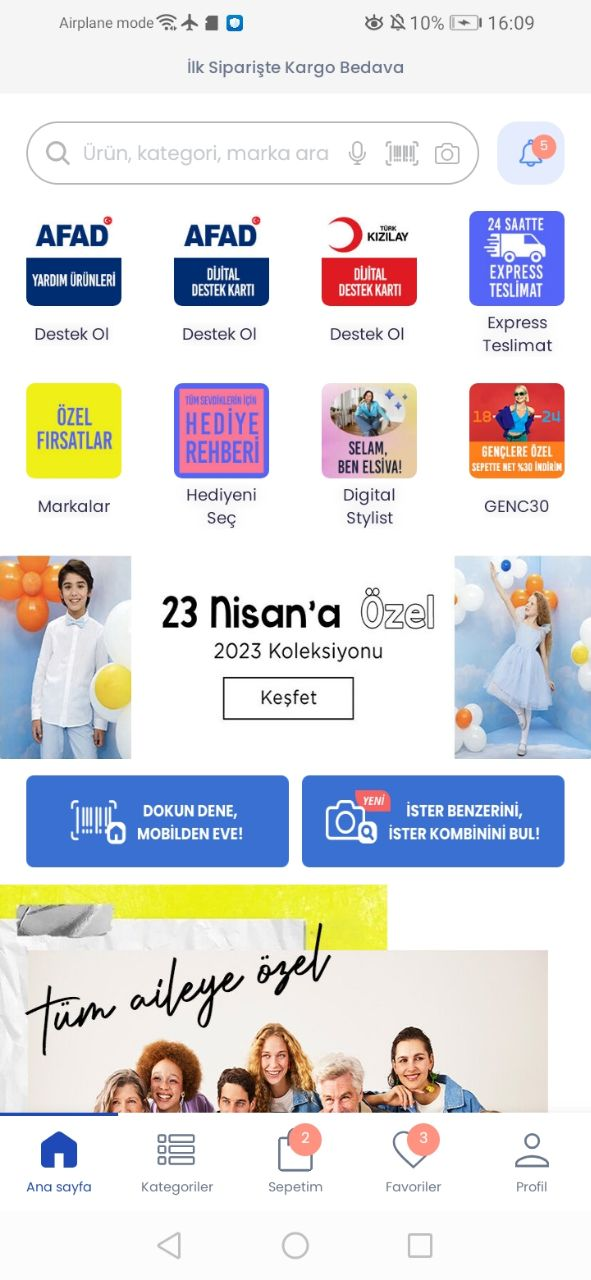
\includegraphics[width=.99\linewidth]
    {images/candidates/LCWaikiki/Home.jpg}
  \end{minipage}
  \begin{minipage}{0.16\textwidth}
    
\includegraphics[width=.99\linewidth]
    {images/candidates/Lamoda/Home.jpg}
  \end{minipage}
  \begin{minipage}{0.16\textwidth}
    
\includegraphics[width=.99\linewidth]
    {images/candidates/DeFacto/Home.jpg}
  \end{minipage}
  \begin{minipage}{0.16\textwidth}
    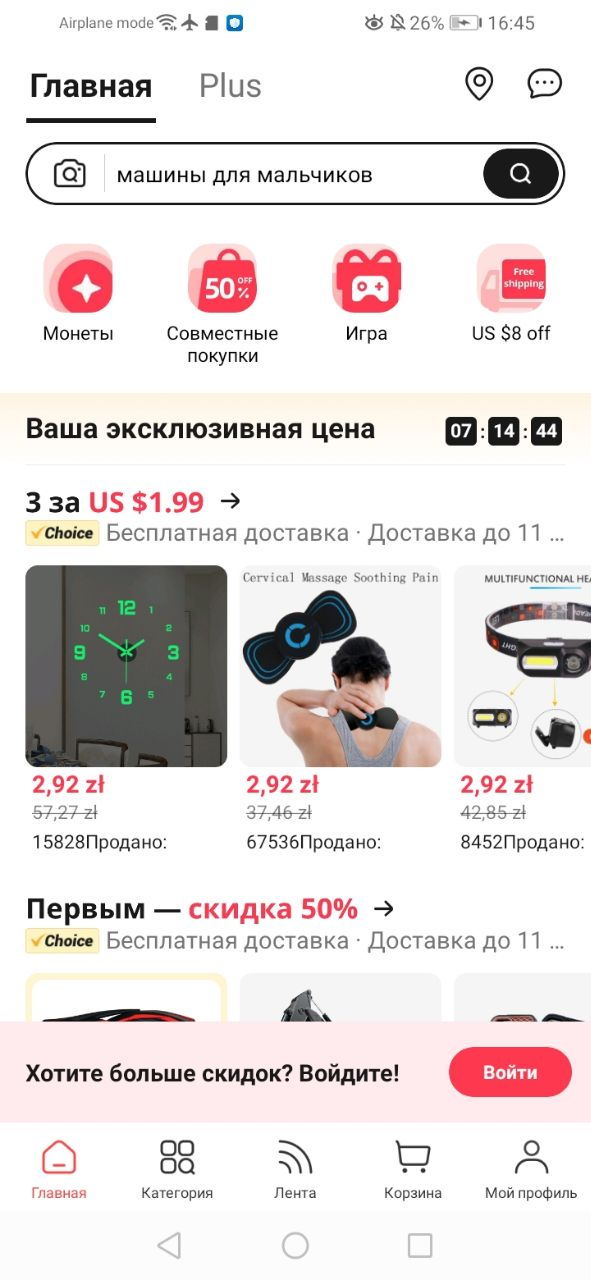
\includegraphics[width=.99\linewidth]
    {images/candidates/AliExpress/Home.jpg}
  \end{minipage}

  \caption{Аналоги главного экрана}\label{fig:analyzHome}
\end{figure}

\begin{figure}[!p]
  \centering

  \begin{minipage}{0.16\textwidth}
    
\includegraphics[width=.99\linewidth]
    {images/candidates/Wildberies/Item.jpg}
  \end{minipage}
  % \begin{minipage}{0.16\textwidth}
  %   \includegraphics[width=.99\linewidth]
  %   {images/candidates/OZby/Item.jpg}
  % \end{minipage}
  % \begin{minipage}{0.16\textwidth}
  %   \includegraphics[width=.99\linewidth]
  %   {images/candidates/LCWaikiki/Item.jpg}
  % \end{minipage}
  \begin{minipage}{0.16\textwidth}
    
\includegraphics[width=.99\linewidth]
    {images/candidates/Lamoda/Item.jpg}
  \end{minipage}
  \begin{minipage}{0.16\textwidth}
    
\includegraphics[width=.99\linewidth]
    {images/candidates/DeFacto/Item.jpg}
  \end{minipage}
  \begin{minipage}{0.16\textwidth}
    
\includegraphics[width=.99\linewidth]
    {images/candidates/AliExpress/Item.jpg}
  \end{minipage}

  \caption{Аналоги экрана с товаром}\label{fig:analyzItem}
\end{figure}

\begin{figure}[!p]
  \centering

  \begin{minipage}{0.16\textwidth}
    
\includegraphics[width=.99\linewidth]
    {images/candidates/Wildberies/ItemCharacteristics.jpg}
  \end{minipage}
  % \begin{minipage}{0.16\textwidth}
  %   \includegraphics[width=.99\linewidth]
  %   {images/candidates/OZby/ItemCharacteristics.jpg}
  % \end{minipage}
  % \begin{minipage}{0.16\textwidth}
  %   \includegraphics[width=.99\linewidth]
  %   {images/candidates/LCWaikiki/ItemCharacteristics.jpg}
  % \end{minipage}
  \begin{minipage}{0.16\textwidth}
    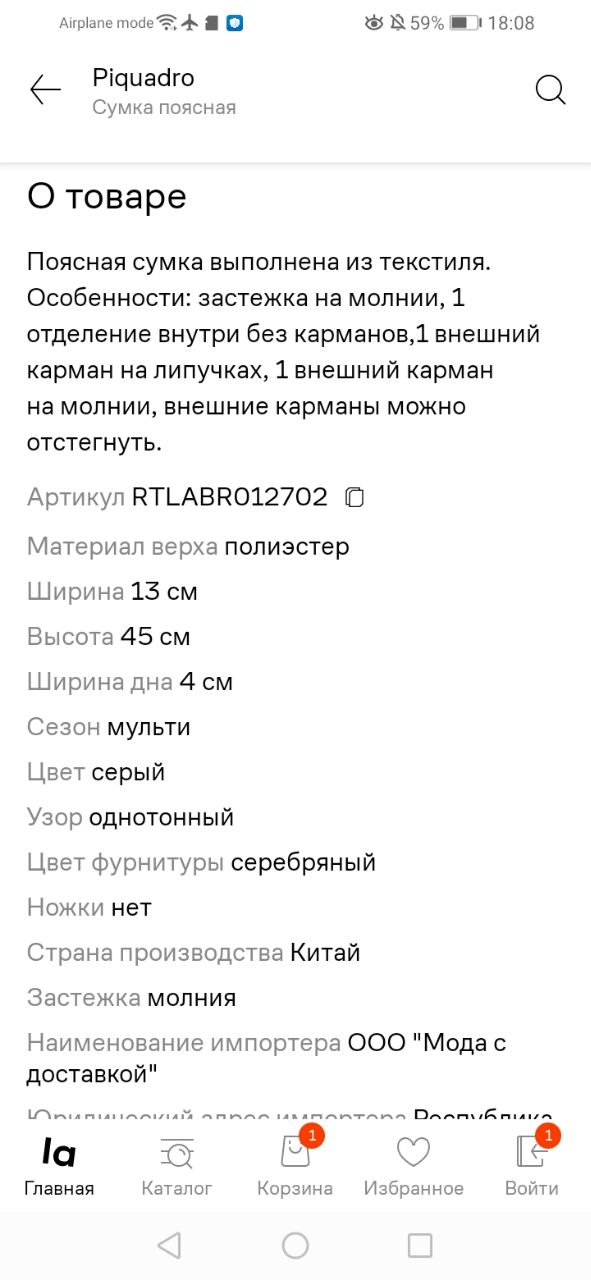
\includegraphics[width=.99\linewidth]
    {images/candidates/Lamoda/ItemCharacteristics.jpg}
  \end{minipage}
  \begin{minipage}{0.16\textwidth}
    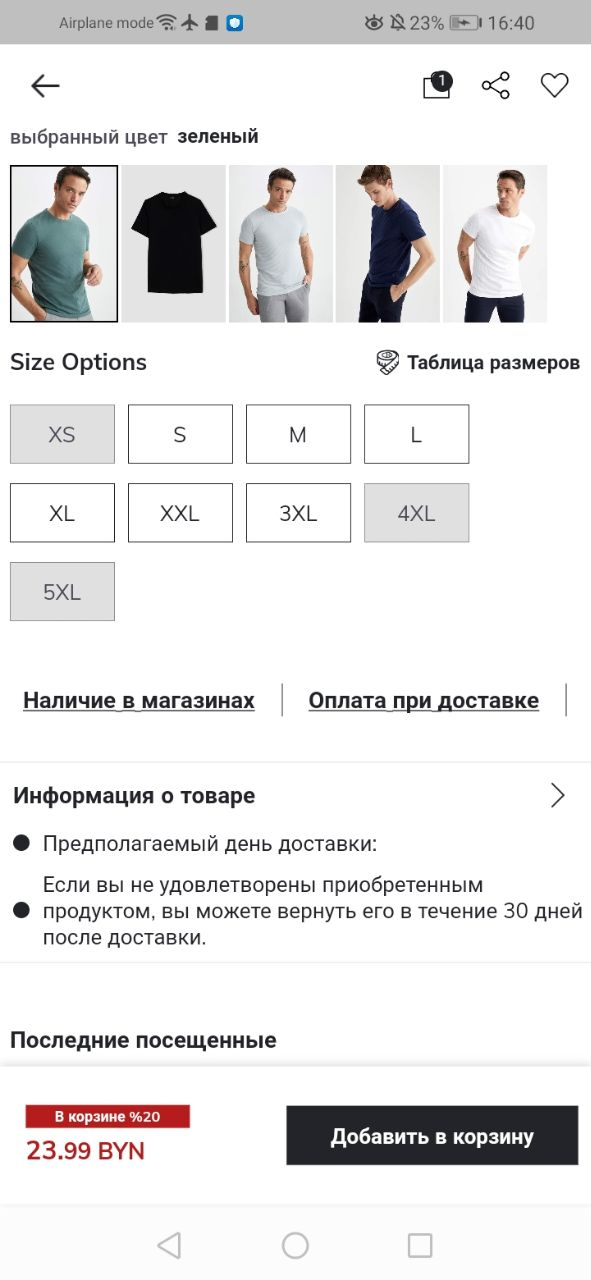
\includegraphics[width=.99\linewidth]
    {images/candidates/DeFacto/ItemCharacteristics.jpg}
  \end{minipage}
  \begin{minipage}{0.16\textwidth}
    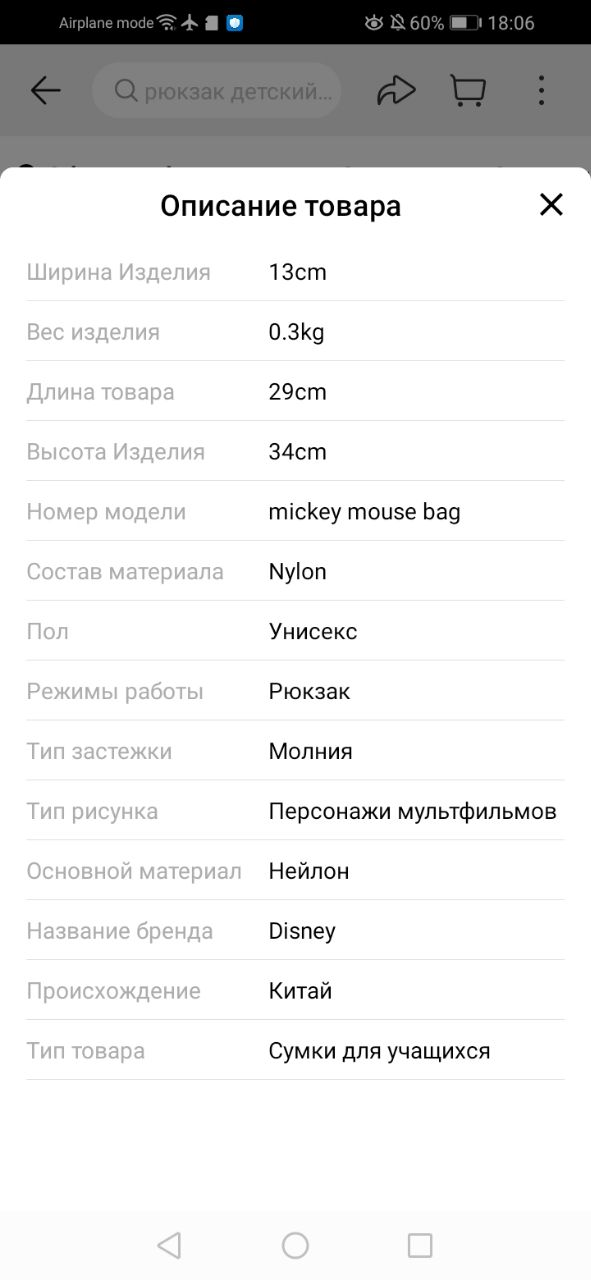
\includegraphics[width=.99\linewidth]
    {images/candidates/AliExpress/ItemCharacteristics.jpg}
  \end{minipage}

  \caption{Примеры описания характиристик номенклатуры}\label{fig:analyzItemCharacteristic}
\end{figure}

\begin{figure}[!p]
  \centering

  \begin{minipage}{0.16\textwidth}
    
\includegraphics[width=.99\linewidth]
    {images/candidates/Wildberies/Basket.jpg}
  \end{minipage}
  % \begin{minipage}{0.16\textwidth}
  %   \includegraphics[width=.99\linewidth]
  %   {images/candidates/OZby/ItemCharacteristics.jpg}
  % \end{minipage}
  \begin{minipage}{0.16\textwidth}
    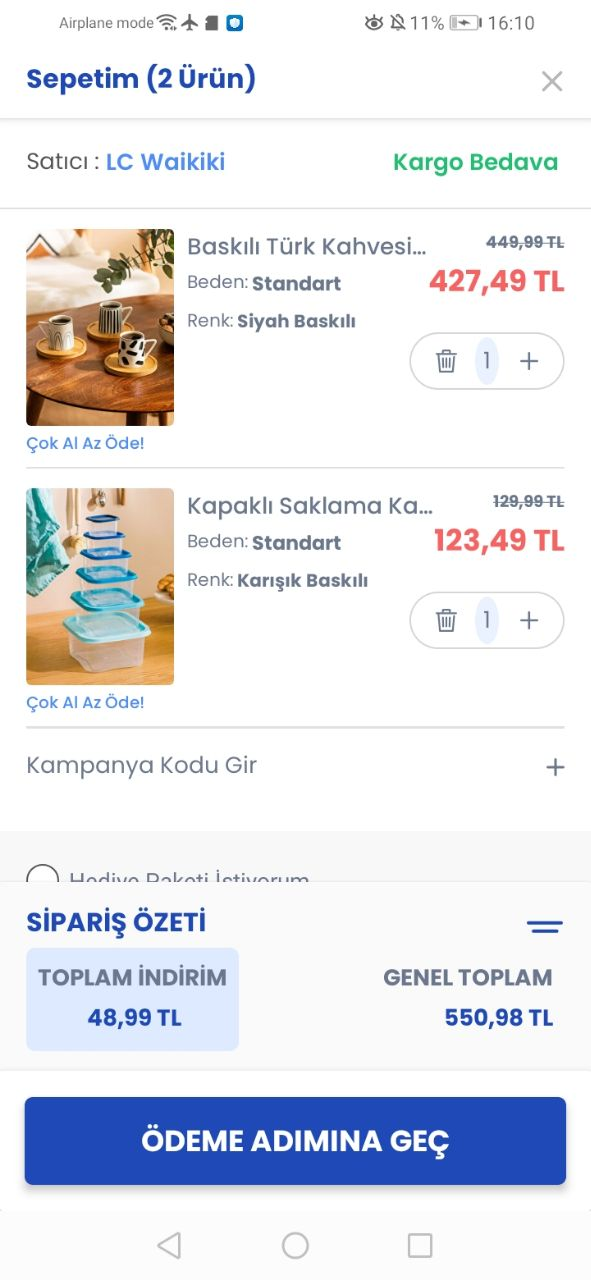
\includegraphics[width=.99\linewidth]
    {images/candidates/LCWaikiki/Basket.jpg}
  \end{minipage}
  \begin{minipage}{0.16\textwidth}
    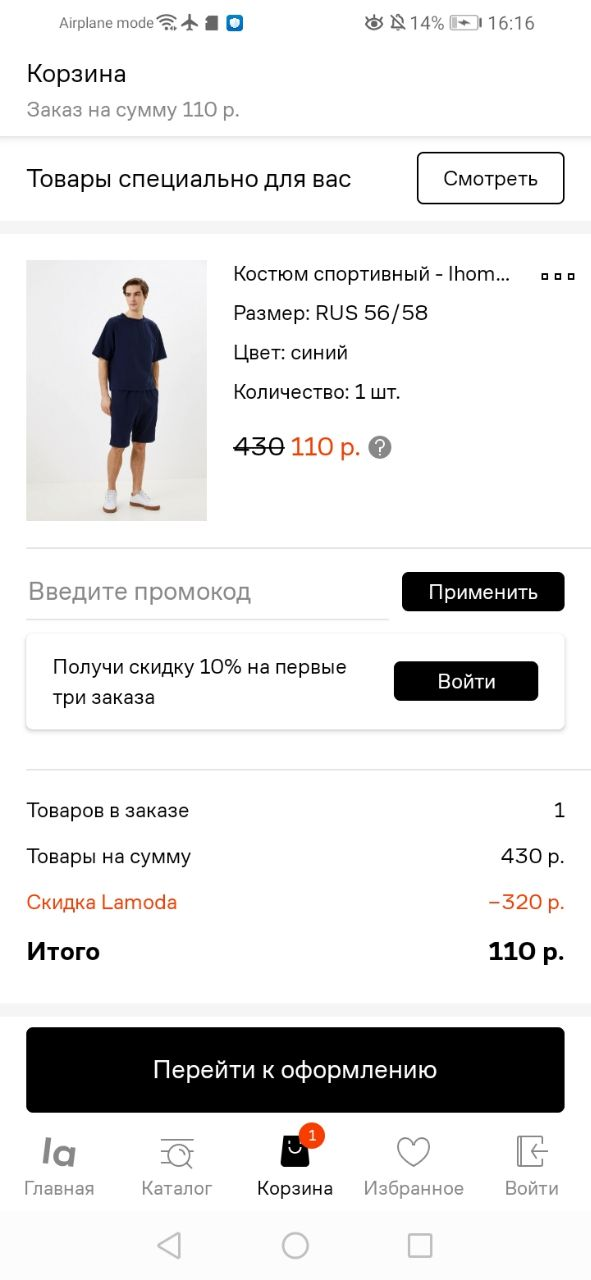
\includegraphics[width=.99\linewidth]
    {images/candidates/Lamoda/Basket.jpg}
  \end{minipage}
  \begin{minipage}{0.16\textwidth}
    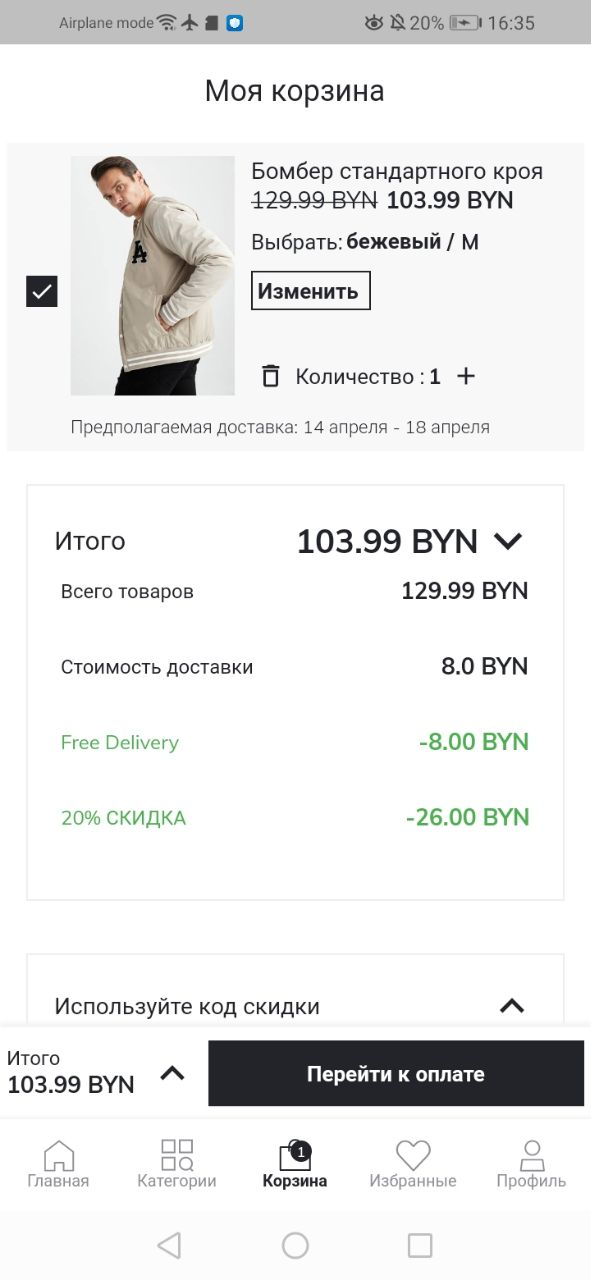
\includegraphics[width=.99\linewidth]
    {images/candidates/DeFacto/Basket.jpg}
  \end{minipage}
  \begin{minipage}{0.16\textwidth}
    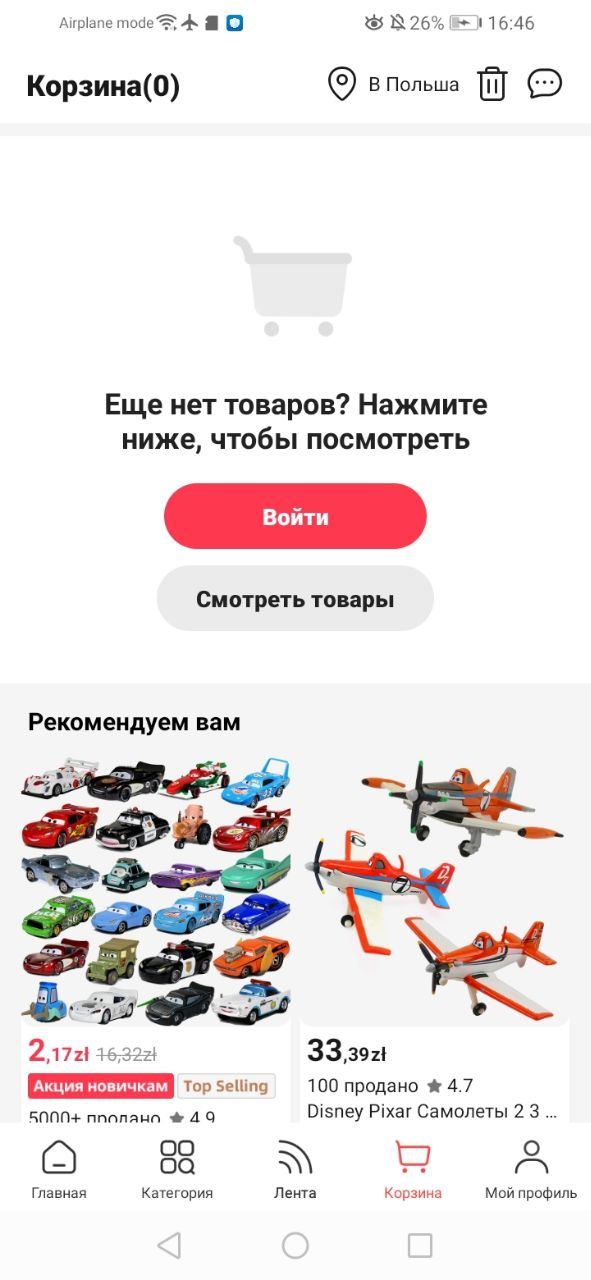
\includegraphics[width=.99\linewidth]
    {images/candidates/AliExpress/Basket.jpg}
  \end{minipage}

  \caption{Примеры оформления корзины с номенклатурой}\label{fig:analyzBasket}
\end{figure}

\begin{figure}[!p]
  \centering

  \begin{minipage}{0.16\textwidth}
    
\includegraphics[width=.99\linewidth]
    {images/candidates/Wildberies/Login.jpg}
  \end{minipage}
  \begin{minipage}{0.16\textwidth}
    
\includegraphics[width=.99\linewidth]
    {images/candidates/OZby/Login.jpg}
  \end{minipage}
  \begin{minipage}{0.16\textwidth}
    
\includegraphics[width=.99\linewidth]
    {images/candidates/LCWaikiki/Login.jpg}
  \end{minipage}
  \begin{minipage}{0.16\textwidth}
    
\includegraphics[width=.99\linewidth]
    {images/candidates/Lamoda/Login.jpg}
  \end{minipage}
  \begin{minipage}{0.16\textwidth}
    
\includegraphics[width=.99\linewidth]
    {images/candidates/DeFacto/Login.jpg}
  \end{minipage}
  % \begin{minipage}{0.16\textwidth}
  %   \includegraphics[width=.99\linewidth]
  %   {images/candidates/AliExpress/Login.jpg}
  % \end{minipage}

  \caption{Аналоги экрана входа}\label{fig:analyzLogin}
\end{figure}

\begin{figure}[!p]
  \centering

  % \begin{minipage}{0.16\textwidth}
  %   \includegraphics[width=.99\linewidth]
  %   {images/candidates/Wildberies/Like.jpg}
  % \end{minipage}
  % \begin{minipage}{0.16\textwidth}
  %   \includegraphics[width=.99\linewidth]
  %   {images/candidates/OZby/Like.jpg}
  % \end{minipage}
  \begin{minipage}{0.16\textwidth}
    
\includegraphics[width=.99\linewidth]
    {images/candidates/LCWaikiki/Like.jpg}
  \end{minipage}
  \begin{minipage}{0.16\textwidth}
    
\includegraphics[width=.99\linewidth]
    {images/candidates/Lamoda/Like.jpg}
  \end{minipage}
  \begin{minipage}{0.16\textwidth}
    
\includegraphics[width=.99\linewidth]
    {images/candidates/DeFacto/Like.jpg}
  \end{minipage}
  % \begin{minipage}{0.16\textwidth}
  %   \includegraphics[width=.99\linewidth]
  %   {images/candidates/AliExpress/Like.jpg}
  % \end{minipage}

  \caption{Примеры экрана избранных}\label{fig:analyzLike}
\end{figure}


\subsection{Обзор используемых технологий}

Нельзя точно уточнить, какие технологии использовались для написания мобильных приложений
WildBerries, OZ.by, LC Waikiki, Lamoda, Defacto,
потому что эта информация не является открытой и не раскрывается компаниями-разработчиками.
Компании могут использовать различные языки программирования и технологии в зависимости от своих потребностей,
бизнес-задач и команд разработки.

Однако, удалось узнать, что мобильное приложение AliExpress
написано на языке программирования Java \cite{AliExpressLang} \cite{AliExpressLangForum}.

Выбор технологий для разработки мобильных приложений зависит от многих факторов,
таких как требования к производительности, функциональные возможности, доступность ресурсов и т.д.
Поэтому разработчикам приходится выбирать технологии, которые лучше всего соответствуют их потребностям.
Однако в целом, для разработки мобильных приложений используются различные языки программирования и фреймворки,
такие как Java, Kotlin, Swift, React Native, Xamarin и др.

\subsection{Выбор средств реализации}

\textbf{React Native} \cite{ReactNativeCliGuide} был выбран из-за его возможностей создания кроссплатформенных мобильных приложений для iOS и Android,
используя только JavaScript (TypeScript) и React-стиль программирования.
Это позволяет существенно сократить время и затраты на разработку, так как код может быть использован на нескольких платформах.
Кроме того, React Native обеспечивает высокую производительность и хорошую оптимизацию для мобильных устройств.

\textbf{MySQL} \cite{MySqlInNestJs} был выбран в качестве базы данных, так как это надежная и широко используемая реляционная СУБД с открытым исходным кодом.
MySQL имеет высокую производительность, масштабируемость и поддерживает все необходимые функции для хранения, организации и извлечения данных.

\textbf{Swagger} \cite{SwaggerInNestJs} был выбран для создания документации API.
Это популярный инструмент для описания и документирования RESTful API.
Swagger обеспечивает удобное взаимодействие между разработчиками,
а также может использоваться для автоматической генерации клиентского кода на различных языках программирования.

\textbf{NestJS} \cite{NestJsGuide} был выбран как фреймворк для создания серверной части приложения.
Он построен на основе TypeScript и использует паттерн MVC (Model-View-Controller) для создания быстрых и масштабируемых веб-приложений.
Nest предоставляет множество инструментов для удобной работы с базами данных, а также обладает высокой производительностью и легким масштабированием.

\textbf{TypeScript} \cite{TypeScriptGuide} был выбран как язык программирования для всего приложения.
Он является надстройкой над JavaScript и обеспечивает статическую типизацию, что улучшает безопасность кода и позволяет облегчить его понимание и сопровождение.
TypeScript также обладает высокой читабельностью кода, что упрощает сопровождение и добавление новых функций в приложение.

\textbf{TypeORM} \cite{TypeORM} \cite{TypeOrmQueryRunner} был выбран в качестве ORM (Object-Relational Map-ping) для работы с базой данных в NestJS.
TypeORM позволяет работать с базами данных разных типов, включая реляционные и NoSQL СУБД, используя объектно-ориентированный подход к работе с данными.
Это позволяет более удобно и эффективно работать с базой данных, а также улучшить производительность и масштабируемость приложения.
TypeORM также предоставляет множество инструментов для управления миграциями базы данных и обновлением схемы данных, что делает процесс разработки и сопровождения приложения более гибким и удобным.

Дополнительно, следует отметить, что TypeORM позволяет создавать миграции базы данных,
что является очень полезной функцией при разработке и сопровождении приложения.

Миграции позволяют автоматически изменять структуру базы данных
без необходимости ручного вмешательства в саму базу данных.

Таким образом, можно легко добавлять новые таблицы,
изменять существующие или удалять их, не беспокоясь о том,
что это может повлиять на работу приложения или привести к ошибкам в работе.

\textbf{В итоге}, React Native, MySQL, Swagger, NestJS, TypeScript и TypeORM были выбраны для создания мобильного приложения под Android из-за их возможностей и надежности,
а также для обеспечения удобной разработки, документирования и масштабирования.

\newpage


\newpage
\section{ПРОЕКТИРОВАНИЕ СИСТЕМЫ}
\subsection*{Варианты использования программы в виде диаграмм прецедентов}

UML диаграмма прецедентов (use case diagram) - это графическое представление функциональности системы, которое показывает,
как взаимодействуют актеры и прецеденты в системе.
Прецеденты представляют собой действия, которые система может выполнять для достижения своих целей,
а актеры - это роли, которые могут взаимодействовать с системой.

Создание диаграммы прецедентов помогает определить функциональные требования к системе и описать ее функциональность в терминах бизнес-процессов.
Это позволяет лучше понять требования пользователей к системе и улучшить ее проектирование.

Описание диаграммы прецедентов позволяет определить, какие действия нужно выполнить для достижения целей пользователей
и какие роли могут взаимодействовать с системой. Это позволяет определить функциональность системы и ее границы,
а также сократить затраты на разработку, путем устранения несущественных или избыточных функций.

В целом, создание диаграммы прецедентов является важным этапом в процессе проектирования системы,
так как она позволяет определить требования к функциональности системы и обеспечить ее соответствие бизнес-потребностям.
Это также позволяет улучшить коммуникацию между разработчиками и пользователями системы, уменьшить вероятность ошибок и повысить качество и эффективность работы системы.

% = = = = = = = =

\subparagraph{Прецедент <<Региcтрация>>} \hspace{0pt}

\underline{Назначение}: регистрация пользователя.

\underline{Исполнители}: мобильный клиент.

\underline{Эндпоинт}: POST /api/v1/users.

\underline{Предусловие}: логин не занят, email не занят.

\underline{Основной поток событий}: HTTP статус 201 (Created) - пользователь зарегистрирован и пользователю пришло на почту ссылка подтверждения.

\underline{Альтернативный поток событий}:

\begin{itemize}
    \item HTTP статус 409 (Conflict) - логин занят другим пользователем;
    \item HTTP статус 409 (Conflict) - email занят другим пользователем;
    \item HTTP статус 500 (Internal Server Error) - транзация не совершена, так как не удалось отправить письмо с ссылкой активации на почту;
    \item HTTP статус 500 (Internal Server Error) - что-то пошло не так на сервере.
\end{itemize}

Диаграмма прецедентов спроектирована в draw.io \cite{drawio} и изображена на рис.~\ref{fig:UML_precedent_registration}.

% = = = = = = = =

\subparagraph{Прецедент <<Активация аккаунта>>} \hspace{0pt}

\underline{Назначение}: активация аккаунта.

\underline{Исполнители}: почтовый клиент.

\underline{Эндпоинт}: GET /api/v1/users/activate-account/:token.

\underline{Предусловие}: не прошло 24 часа.

\underline{Основной поток событий}: HTTP статус 200 (OK) - пользователь подтвердил зарегистрированный аккаунт.

\underline{Альтернативный поток событий}:

\begin{itemize}
    \item HTTP статус 404 (Not Found) - ссылка не действительна, так как прошло 24 часа (токен просрочен);
    \item HTTP статус 404 (Not Found) - ссылка не действительна, так как токен поддельный (токен не прошел проверку валидности);
    \item HTTP статус 404 (Not Found) - ссылка не действительна, так как токен не зарегстрирован в БД (токен прошел проверку, но его нет в БД)
    \item HTTP статус 404 (Not Found) - ссылка не действительна, так как аккаунт был активирован;
    \item HTTP статус 500 (Internal Server Error) - не совершено обновление статуса пользователя;
    \item HTTP статус 500 (Internal Server Error) - что-то пошло не так на сервере.
\end{itemize}

Диаграмма прецедентов спроектирована в draw.io \cite{drawio} и изображена на рис.~\ref{fig:UML_precedent_registration}.

% = = = = = = = =

\begin{figure}[!htb]
    \centering

    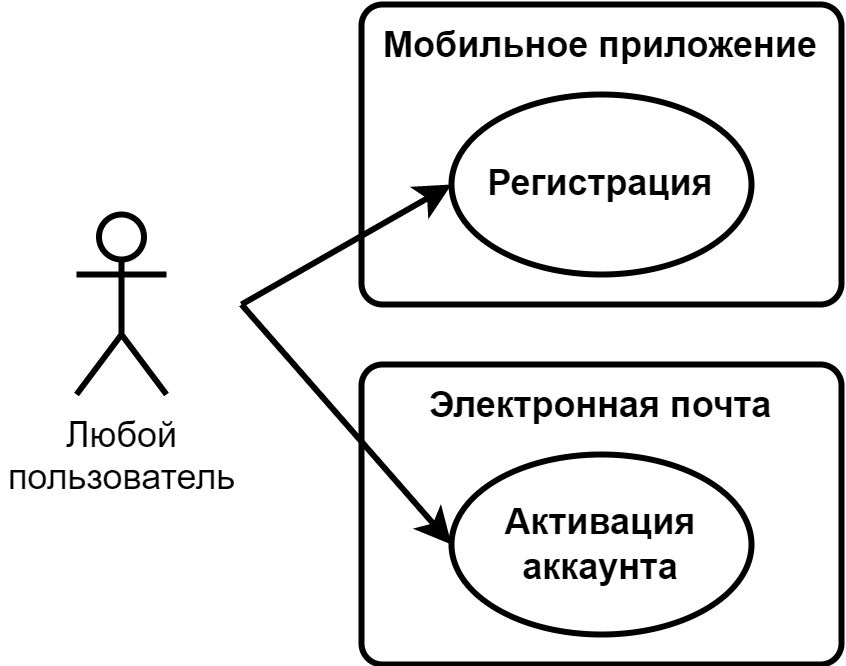
\includegraphics[width=18cm]
    {images/UML/UML_precedent_registration.png}

    \caption{Диаграмма прецедентов для регистрации}

    \label{fig:UML_precedent_registration}
\end{figure}

% = = = = = = = =

\subparagraph{Прецедент <<Заявка на смену электронной почты>>} \hspace{0pt}

\underline{Назначение}: смена электронной почты на новую.

\underline{Исполнители}: мобильный клиент.

\underline{Эндпоинт}: PATCH /api/v1/users/change-email.

\underline{Предусловие}: у пользователя есть токен доступа (access token).

\underline{Основной поток событий}: HTTP статус 200 (OK) - заявка отправлена на новую почту и предупреждение отправлено на старую почту.

\underline{Альтернативный поток событий}:

\begin{itemize}
    \item HTTP статус 401 (Unauthorized) - токен доступа просрочен;
    \item HTTP статус 401 (Unauthorized) - токен доступа не передан;
    \item HTTP статус 409 (Conflict) - новая почта совпадает с текущей;
    \item HTTP статус 429 (To Many Request) - слишком много запросов о смене электроной почты за не прошедшие 3 часа;
    \item HTTP статус 500 (Internal Server Error) - транзация не совершена, так как нет таблицы в БД (не сохранения запись о смене старой электронной почты на новую)
    \item HTTP статус 500 (Internal Server Error) - транзация не совершена, так как не отправлено письмо на новую и старую почту;
    \item HTTP статус 500 (Internal Server Error) - что-то пошло не так на сервере.
\end{itemize}

Диаграмма прецедентов изображены на рис.~\ref{fig:UML_precedent_change_email}.

% = = = = = = = =

\subparagraph{Прецедент <<Подтверждение смены электронной почты>>} \hspace{0pt}

\underline{Назначение}: подтверждение смены электронной почты.

\underline{Исполнители}: электронаая почта.

\underline{Эндпоинт}: GET /api/v1/users/change-email/:token/confirm.

\underline{Предусловие}: не прошло 3 часа.

\underline{Основной поток событий}: HTTP статус 200 (OK) - электронная почта изменена на новую.

\underline{Альтернативный поток событий}:

\begin{itemize}
    \item HTTP статус 404 (Not Found) - сылка не действительна, так как прошло 3 часа (токен просрочен);
    \item HTTP статус 404 (Not Found) - ссылка не действительна, так как токен подделан (токен не прошел валидацию);
    \item HTTP статус 404 (Not Found) - ссылка не действительна, так как токена не зарегистрирован в БД;
    \item HTTP статус 404 (Not Found) - ссылка не действительна, так как почта была сменена, либо заявка на смену почты была отклонена;
    \item HTTP статус 500 (Internal Server Error) - транзация не совернеша (заявка не отмечена закрытой, пользователю не поменял email на новый);
    \item HTTP статус 500 (Internal Server Error) - что-то пошло не так на сервере.
\end{itemize}

Диаграмма прецедентов изображены на рис.~\ref{fig:UML_precedent_change_email}.

% = = = = = = = =

\subparagraph{Прецедент <<Отмена заявки смены электронной почты>>} \hspace{0pt}

\underline{Назначение}: Отмена заявки смены электронной почты.

\underline{Исполнители}: электронная почта.

\underline{Эндпоинт}: GET /api/v1/users/change-email/:token/delete.

\underline{Предусловие}: не прошло 3 часа.

\underline{Основной поток событий}: HTTP статус 200 (OK) - заявка на смену электронной почты отменена.

\underline{Альтернативный поток событий}:

\begin{itemize}
    \item HTTP статус 404 (Not Found) - ссылка не действительна, так как прошло 3 часа (токен просрочен);
    \item HTTP статус 404 (Not Found) - ссылка не действительна, так как токен подделан (токен не прошел валидацию);
    \item HTTP статус 404 (Not Found) - ссылка не действительна, так как токен не зарегистрирован в БД;
    \item HTTP статус 404 (Not Found) - ссылка не действительна, так как почта была сменена, либо заявка на смену почты была отклонена;
    \item HTTP статус 500 (Internal Server Error) - нет таблицы в БД;
    \item HTTP статус 500 (Internal Server Error) - что-то пошло не так на сервере.
\end{itemize}

Диаграмма прецедентов изображены на рис.~\ref{fig:UML_precedent_change_email}.

% = = = = = = = =

\begin{figure}[!htb]
    \centering

    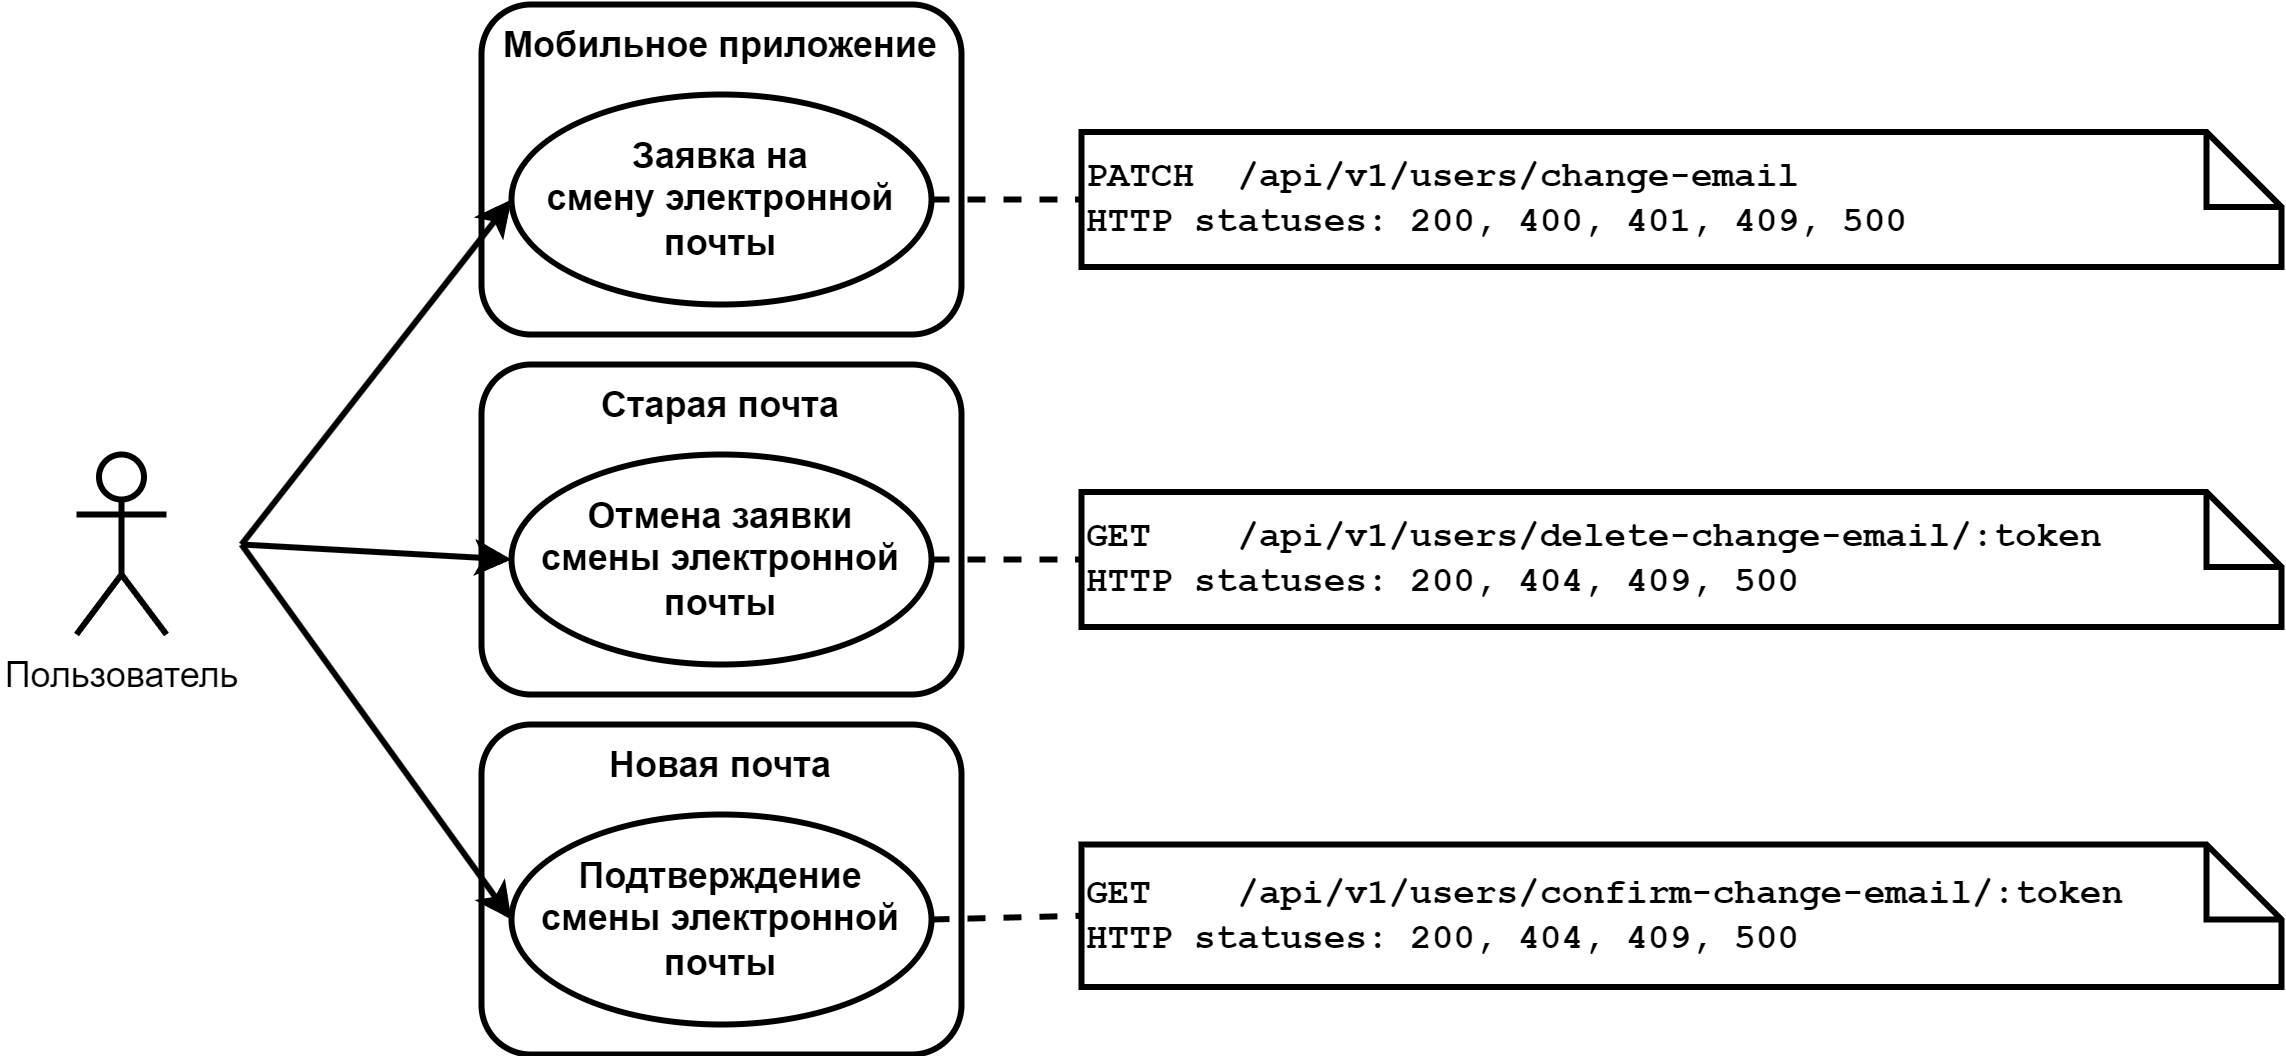
\includegraphics[width=18cm]
    {images/UML/UML_precedent_change_email.png}

    \caption{Диаграмма прецедентов для смены электронной почты}

    \label{fig:UML_precedent_change_email}
\end{figure}

% = = = = = = = =

\subparagraph{Прецедент <<Забыли пароль>>} \hspace{0pt}

\underline{Назначение}: на почту прийдет логин и новый сгенерированый пароль.

\underline{Исполнители}: мобильный клиент.

\underline{Эндпоинт}: POST /api/v1/users/forget-password.

\underline{Предусловие}: у пользователя есть токен доступа (access token).

\underline{Основной поток событий}: HTTP статус 200 (OK) - на электронную почту отправлен логин и новый сгенерированный пароль.

\underline{Альтернативный поток событий}:

\begin{itemize}
    \item HTTP статус 409 (Conflict) - пользователя с такой электронной почтой не существует;
    \item HTTP статус 500 (Internal Server Error) - транзация не совернеша, так как сгенерированный пароль не записался в БД;
    \item HTTP статус 500 (Internal Server Error) - транзация не совернеша, так как письмо с логином и паролем не отправлено на электронную почту;
    \item HTTP статус 500 (Internal Server Error) - что-то пошло не так на сервере.
\end{itemize}

Диаграмма прецедентов изображены на рис.~\ref{fig:UML_precedent_change_password}.

% = = = = = = = =

\subparagraph{Прецедент <<Смена пароля>>} \hspace{0pt}

\underline{Назначение}: смена пароля.

\underline{Исполнители}: мобильный клиент.

\underline{Эндпоинт}: PATCH /api/v1/users/change-password.

\underline{Предусловие}: у пользователя есть токен доступа (access token), пользователь указал верно старый пароль.

\underline{Основной поток событий}: HTTP статус 200 (OK) - пароль изменен. 

\underline{Альтернативный поток событий}:

\begin{itemize}
    \item HTTP статус 409 (Conflict) - не тот старый пароль;
    \item HTTP статус 500 (Internal Server Error) - транзация не совернеша, так как новый пароль не записан в БД;
    \item HTTP статус 500 (Internal Server Error) - транзация не совернеша, так как не удалось завершить все сессии;
    \item HTTP статус 500 (Internal Server Error) - что-то пошло не так на сервере.
\end{itemize}

Диаграмма прецедентов изображены на рис.~\ref{fig:UML_precedent_change_password}.

% = = = = = = = =

\begin{figure}[!htb]
    \centering

    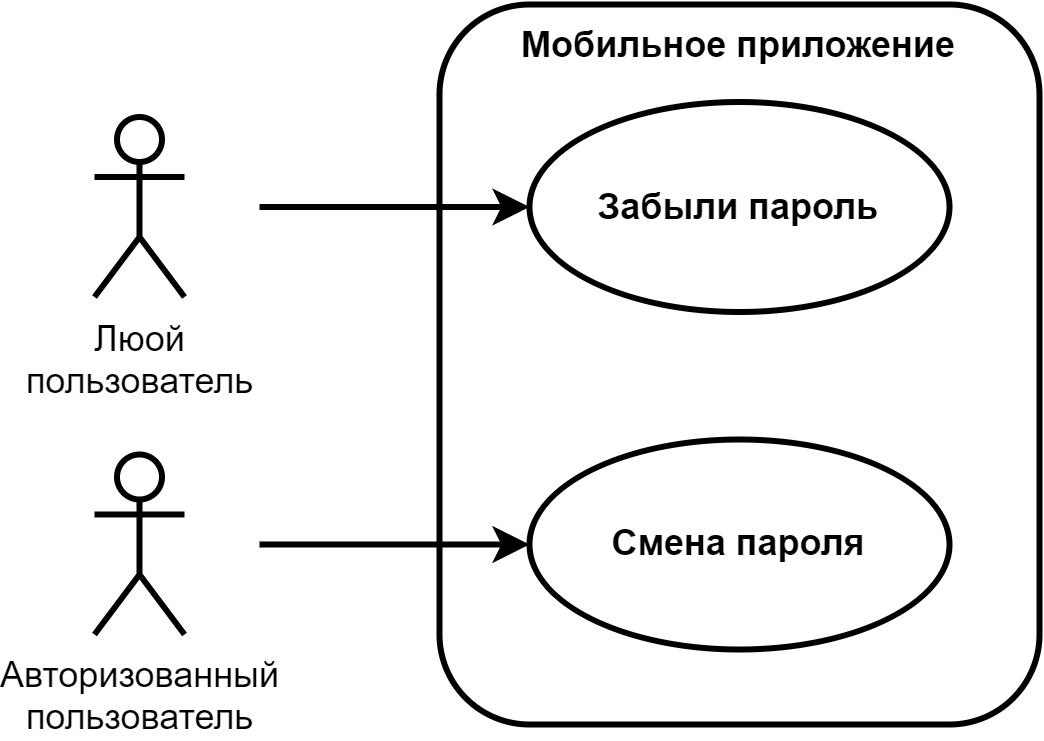
\includegraphics[width=18cm]
    {images/UML/UML_precedent_change_password.png}

    \caption{Диаграмма прецедентов для смены пароля}

    \label{fig:UML_precedent_change_password}
\end{figure}

% = = = = = = = =

\subparagraph{Прецедент <<Вход в аккаунт>>} \hspace{0pt}

\underline{Назначение}: ввойти в аккаунт.

\underline{Исполнители}: мобильный клиент.

\underline{Эндпоинт}: POST /api/v1/sessions.

\underline{Предусловие}: пользователь указал существующий логин и верный пароль.

\underline{Основной поток событий}: HTTP статус 201 (Created) - пользователь авторизовался (получил access и refresh токены). 

\underline{Альтернативный поток событий}:

\begin{itemize}
    \item HTTP статус 409 (Conflict) - нет пользователя с таким логином;
    \item HTTP статус 409 (Conflict) - не тот пароль.
    \item HTTP статус 500 (Internal Server Error) - что-то пошло не так на сервере.
\end{itemize}

Диаграмма прецедентов изображены на рис.~\ref{fig:UML_precedent_sessions}.

% = = = = = = = =

\subparagraph{Прецедент <<Получаем список сессий>>} \hspace{0pt}

\underline{Назначение}: получить список сессий.

\underline{Исполнители}: мобильный клиент.

\underline{Эндпоинт}: GET /api/v1/sessions.

\underline{Предусловие}: у пользователя есть токен доступа (access token).

\underline{Основной поток событий}: HTTP статус 200 (OK) - получили список ip и устройств. 

\underline{Альтернативный поток событий}: 

\begin{itemize}
    \item HTTP статус 401 (Unauthorized) - access токен просрочен;
    \item HTTP статус 401 (Unauthorized) - access токен не переда;
    \item HTTP статус 500 (Internal Server Error) - что-то пошло не так на сервере.
\end{itemize}

Диаграмма прецедентов изображены на рис.~\ref{fig:UML_precedent_sessions}.

% = = = = = = = =

\subparagraph{Прецедент <<Обновление токена доступа>>} \hspace{0pt}

\underline{Назначение}: обновить просроченый или потеряный токен доступа имея токено обновления.

\underline{Исполнители}: мобильный клиент.

\underline{Эндпоинт}: PATCH /api/v1/sessions.

\underline{Предусловие}: у пользователя есть токен обновления (refresh token).

\underline{Основной поток событий}: HTTP статус 200 (OK) - получили новый access токен. 

\underline{Альтернативный поток событий}:

\begin{itemize}
    \item HTTP статус 401 (Unauthorized) - refresh токен просрочен;
    \item HTTP статус 401 (Unauthorized) - refresh токен не передан;
    \item HTTP статус 500 (Internal Server Error) - что-то пошло не так на сервере.
\end{itemize}

Диаграмма прецедентов изображены на рис.~\ref{fig:UML_precedent_sessions}.

% = = = = = = = =

\subparagraph{Прецедент <<Завершение всех сессий>>} \hspace{0pt}

\underline{Назначение}: закрыть все сессии.

\underline{Исполнители}: мобильный клиент.

\underline{Эндпоинт}: DELETE /api/v1/sessions.

\underline{Предусловие}: у пользователя есть токен доступа (access token).

\underline{Основной поток событий}: HTTP статус 200 (OK) - закрыли все сессии. 

\underline{Альтернативный поток событий}:

\begin{itemize}
    \item HTTP статус 401 (Unauthorized) - access токен просрочен;
    \item HTTP статус 401 (Unauthorized) - access токен не передан;
    \item HTTP статус 500 (Internal Server Error) - что-то пошло не так на сервере.
\end{itemize}

Диаграмма прецедентов изображены на рис.~\ref{fig:UML_precedent_sessions}.

% = = = = = = = =

\subparagraph{Прецедент <<Завершение сессии по id>>} \hspace{0pt}

\underline{Назначение}: закрыть сессию по id.

\underline{Исполнители}: мобильный клиент.

\underline{Эндпоинт}: DELETE /api/v1/sessions/:id.

\underline{Предусловие}: у пользователя есть токен доступа (access token).

\underline{Основной поток событий}: HTTP статус 200 (OK) - закрыли сессию по id. 

\underline{Альтернативный поток событий}:

\begin{itemize}
    \item HTTP статус 401 (Unauthorized) - access токен просрочен;
    \item HTTP статус 401 (Unauthorized) - access токен не передан;
    \item HTTP статус 500 (Internal Server Error) - что-то пошло не так на сервере.
\end{itemize}

Диаграмма прецедентов изображены на рис.~\ref{fig:UML_precedent_sessions}.

% = = = = = = = =

\begin{figure}[!htb]
    \centering

    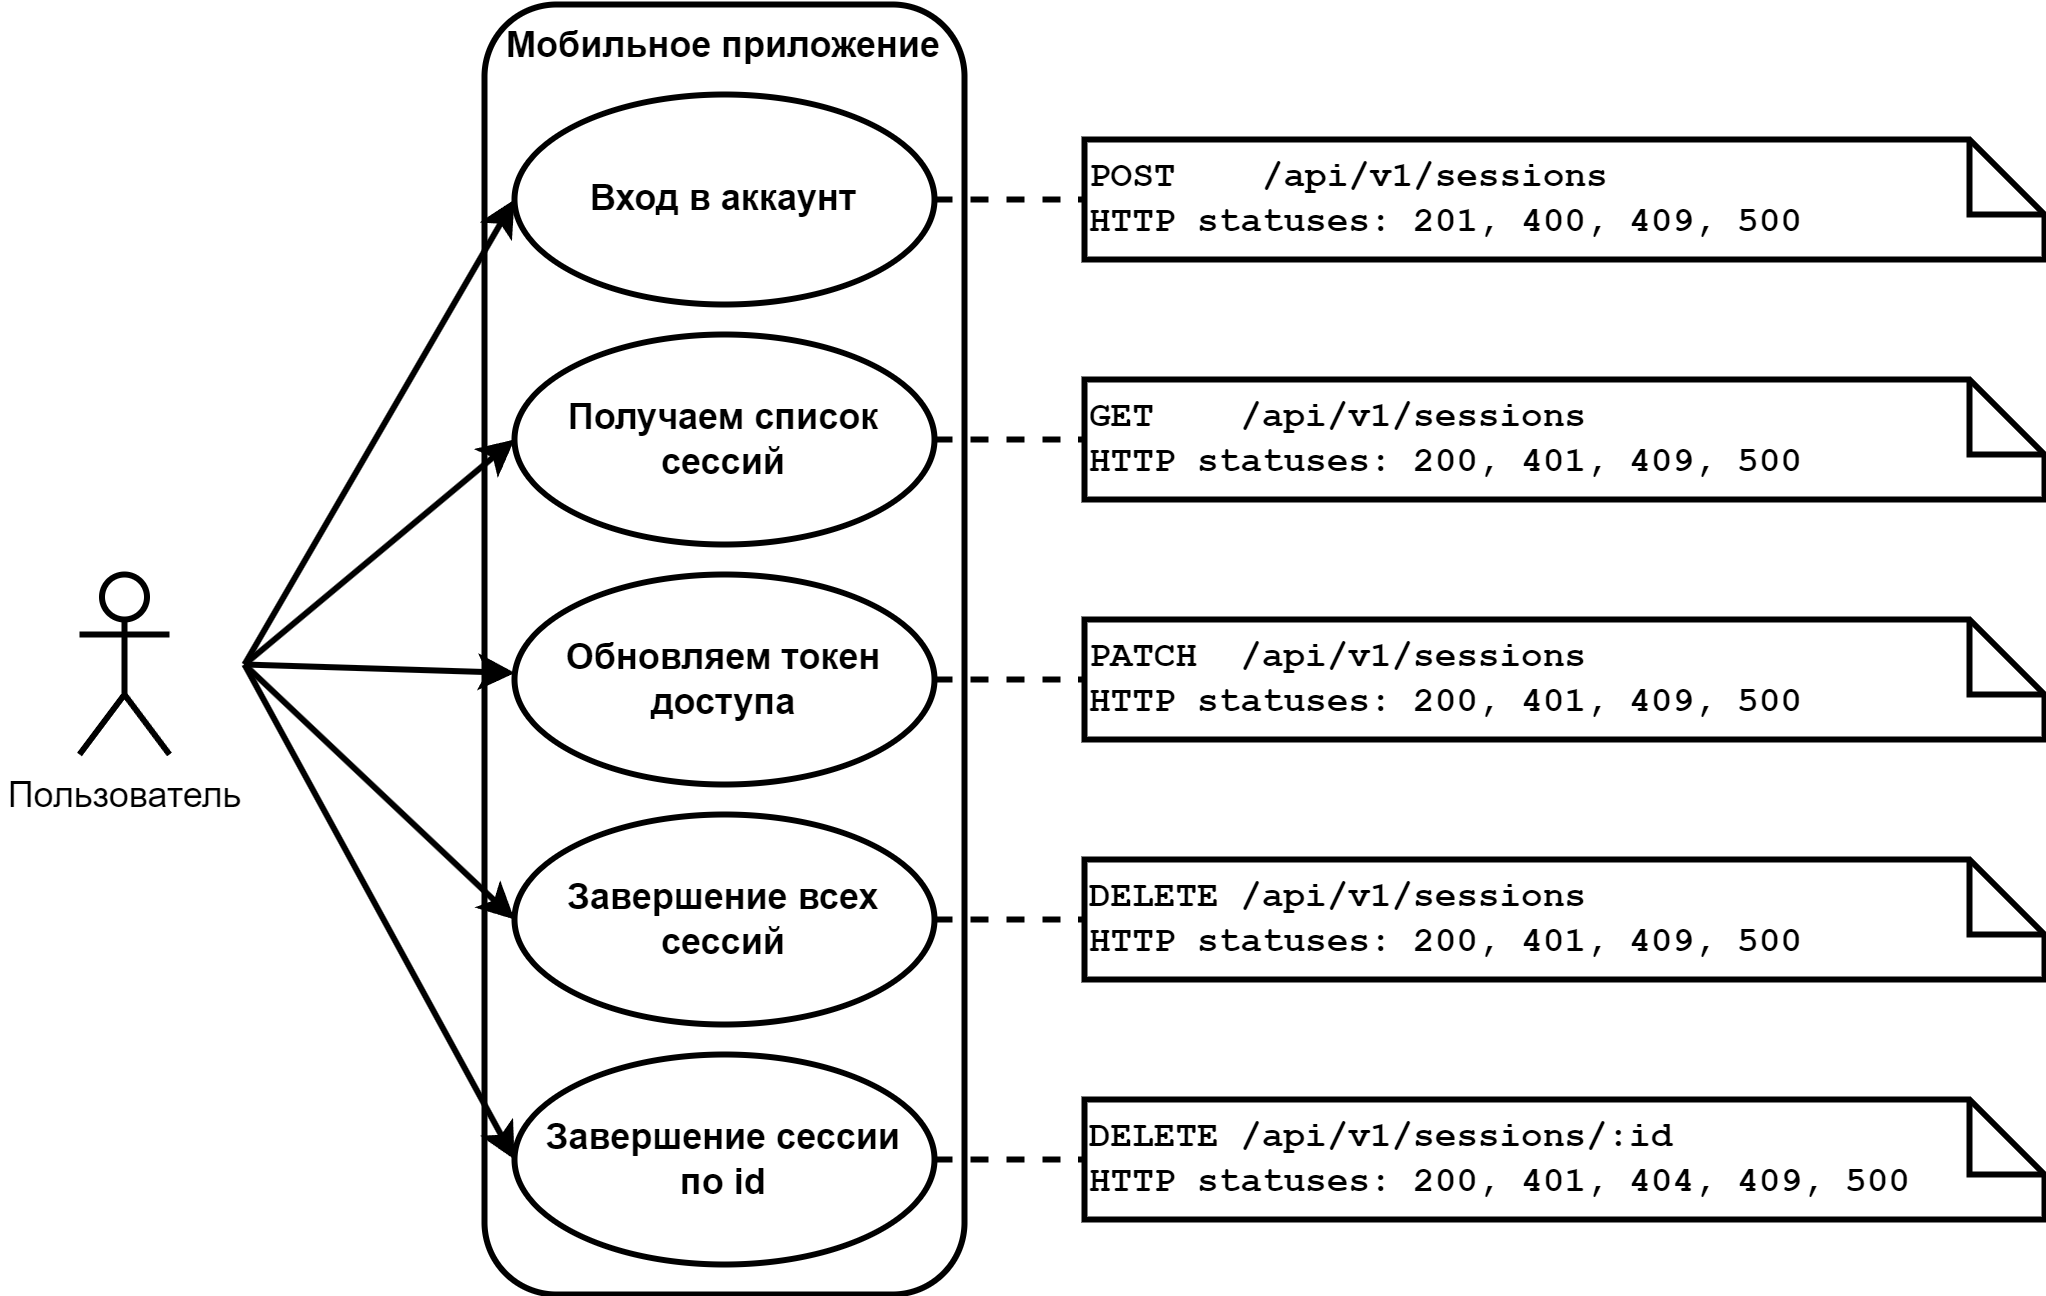
\includegraphics[width=18cm]
    {images/UML/UML_precedent_sessions.png}

    \caption{Диаграмма прецедентов для смены электронной почты}

    \label{fig:UML_precedent_sessions}
\end{figure}

% = = = = = = = =

\subparagraph{Прецедент <<Создание заявки товаров(-а)>>} \hspace{0pt}

\underline{Назначение}: создание заявка на отбор товаров(-а).

\underline{Исполнители}: мобильный клиент.

\underline{Эндпоинт}: POST /api/v1/order-items.

\underline{Предусловие}: у пользователя есть токен доступа (access token).

\underline{Основной поток событий}: HTTP статус 200 (OK) - пользователь оставил заявку на отбор товаров(-а). 

\underline{Альтернативный поток событий}:

\begin{itemize}
    \item HTTP статус 401 (Unauthorized) - пользователь не указал токен доступа;
    \item HTTP статус 401 (Unauthorized) - пользователь указал просроченый токен доступа (нет в БД);
    \item HTTP статус 500 (Internal Server Error) - что-то пошло не так на сервере.
\end{itemize}

Диаграмма прецедентов изображены на рис.~\ref{fig:UML_precedent_order_items}.

% = = = = = = = =

\subparagraph{Прецедент <<Просмотр списка заявок>>} \hspace{0pt}

\underline{Назначение}: просмотр список заявок.

\underline{Исполнители}: мобильный клиент.

\underline{Эндпоинт}: GET /api/v1/order-items.

\underline{Предусловие}: у пользователя есть токен доступа (access token).

\underline{Основной поток событий}: HTTP статус 200 (OK) - пользователь получил список заявок. 

\underline{Альтернативный поток событий}:

\begin{itemize}
    \item HTTP статус 401 (Unauthorized) - пользователь не указал токен доступа;
    \item HTTP статус 401 (Unauthorized) - пользователь указал просроченый токен доступа (нет в БД);
    \item HTTP статус 500 (Internal Server Error) - что-то пошло не так на сервере.
\end{itemize}

Диаграмма прецедентов изображены на рис.~\ref{fig:UML_precedent_order_items}.

% = = = = = = = =

\subparagraph{Прецедент <<Просмотр заявки по uuid>>} \hspace{0pt}

\underline{Назначение}: просмотр заказаных товаров.

\underline{Исполнители}: мобильный клиент.

\underline{Эндпоинт}: GET /api/v1/order-items/:uuid.

\underline{Предусловие}: у пользователя есть токен доступа (access token).

\underline{Основной поток событий}: HTTP статус 200 (OK) - пользователь получил список товаров в заявке. 

\underline{Альтернативный поток событий}:

\begin{itemize}
    \item HTTP статус 401 (Unauthorized) - пользователь не указал токен доступа;
    \item HTTP статус 401 (Unauthorized) - пользователь указал просроченый токен доступа (нет в БД);
    \item HTTP статус 404 (Not Found) - такой заявки не существует;
    \item HTTP статус 500 (Internal Server Error) - что-то пошло не так на сервере.
\end{itemize}

Диаграмма прецедентов изображены на рис.~\ref{fig:UML_precedent_order_items}.

% = = = = = = = =

\subparagraph{Прецедент <<Отмена заявки по uuid>>} \hspace{0pt}

\underline{Назначение}: отмена заявки.

\underline{Исполнители}: мобильный клиент.

\underline{Эндпоинт}: DELETE /api/v1/order-items/:uuid.

\underline{Предусловие}: у пользователя есть токен доступа (access token).

\underline{Основной поток событий}: HTTP статус 200 (OK) - пользователь отменил заявку. 

\underline{Альтернативный поток событий}:

\begin{itemize}
    \item HTTP статус 401 (Unauthorized) - пользователь не указал токен доступа;
    \item HTTP статус 401 (Unauthorized) - пользователь указал просроченый токен доступа (нет в БД);
    \item HTTP статус 404 (Not Found) - такой заявки не существует;
    \item HTTP статус 500 (Internal Server Error) - что-то пошло не так на сервере.
\end{itemize}

Диаграмма прецедентов изображены на рис.~\ref{fig:UML_precedent_order_items}.

% = = = = = = = =

\subparagraph{Прецедент <<Просмотр статуса отбора товаров(-а)>>} \hspace{0pt}

\underline{Назначение}: просмотреть статус отбора товаров(-а).

\underline{Исполнители}: мобильный клиент, браузер.

\underline{Эндпоинт}: GET /api/v1/order-items/:uuid/status.

\underline{Предусловие}: uuid заявки найден в БД.

\underline{Основной поток событий}: HTTP статус 200 (OK) - пользователь получил список статусов о состоянии отбора товаров(-а). 

\underline{Альтернативный поток событий}:

\begin{itemize}
    \item HTTP статус 404 (Not Found) - заявка не найдена;
    \item HTTP статус 500 (Internal Server Error) - что-то пошло не так на сервере.
\end{itemize}

Диаграмма прецедентов изображены на рис.~\ref{fig:UML_precedent_order_items}.

% = = = = = = = =

\begin{figure}[!htb]
    \centering

    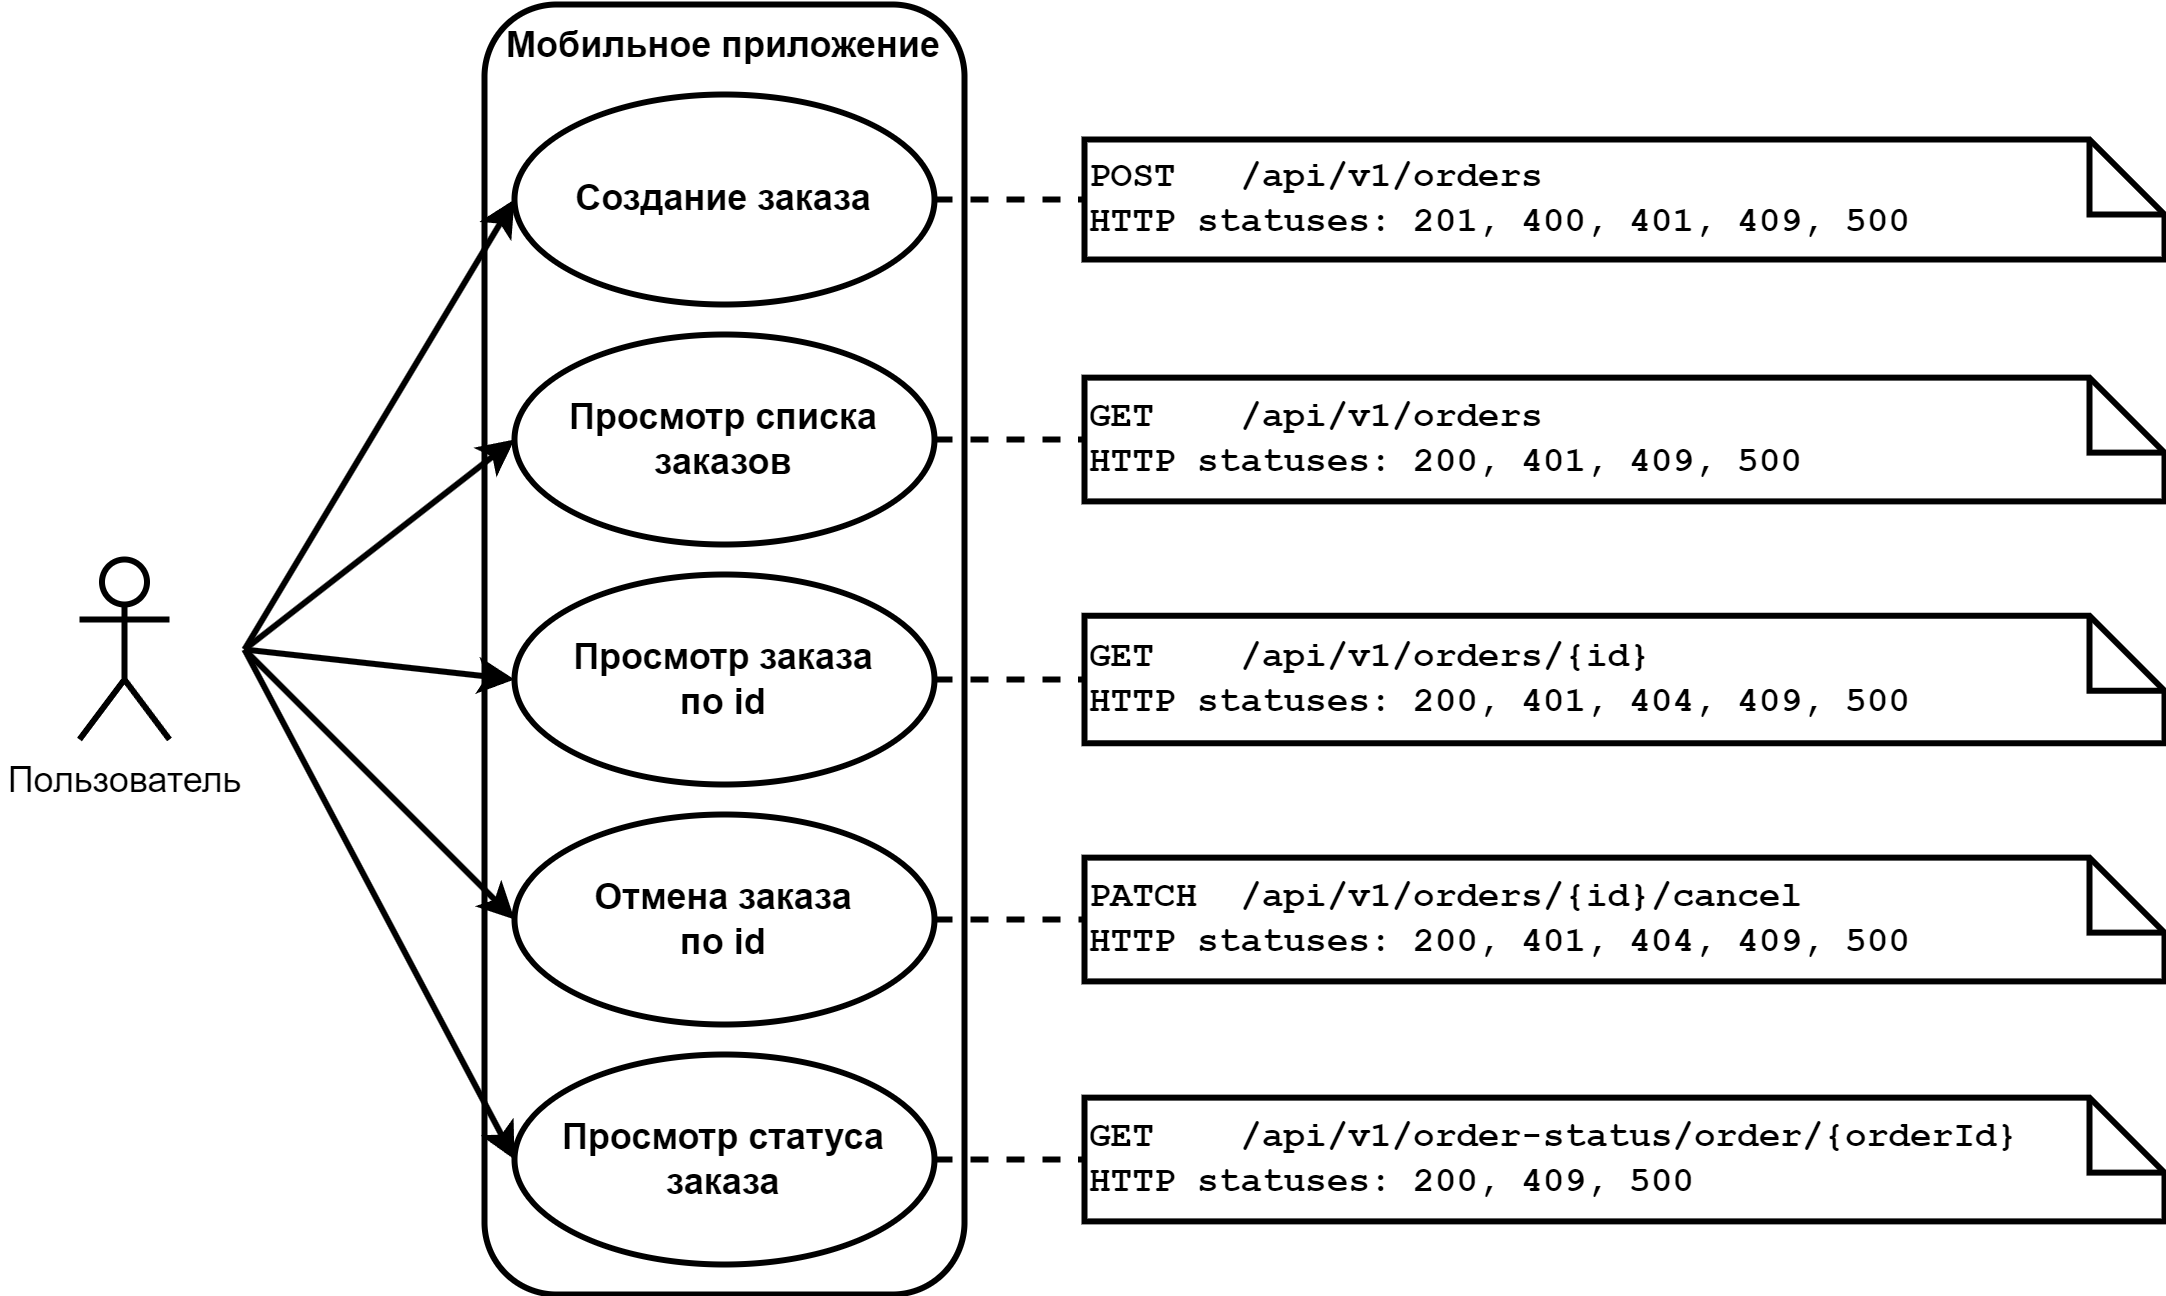
\includegraphics[width=18cm]
    {images/UML/UML_precedent_order_items.png}

    \caption{Диаграмма прецедентов для заявки отбора товаров}

    \label{fig:UML_precedent_order_items}
\end{figure}

% = = = = = = = =

\subparagraph{Прецедент <<Создание номенклатуры>>} \hspace{0pt}

\underline{Назначение}: запись номенклатуры в БД.

\underline{Исполнители}: администратор, браузер.

\underline{Эндпоинт}: POST /api/v1/items.

\underline{Предусловие}: у пользователя есть токен доступа и роль admin.

\underline{Основной поток событий}: HTTP статус 201 (Created) - администратор создал номенклатуру в БД. 

\underline{Альтернативный поток событий}:
HTTP статус 500 (Internal Server Error) - что-то пошло не так на сервере.

Диаграмма прецедентов изображены на рис.~\ref{fig:UML_precedent_items}.

% = = = = = = = =

\subparagraph{Прецедент <<Просмотр списка номенклатуры>>} \hspace{0pt}

\underline{Назначение}: просмотр списка номенклатуры.

\underline{Исполнители}: мобильный клиент, браузер.

\underline{Эндпоинт}: GET /api/v1/items.

% \underline{Предусловие}: 

\underline{Основной поток событий}: HTTP статус 200 (OK) - пользователь получил список номенклатуры. 

\underline{Альтернативный поток событий}:
HTTP статус 500 (Internal Server Error) - что-то пошло не так на сервере.

Диаграмма прецедентов изображены на рис.~\ref{fig:UML_precedent_items}.

% = = = = = = = =

\subparagraph{Прецедент <<Просмотр номенклатуры по uuid>>} \hspace{0pt}

\underline{Назначение}: просмотр определённой номенклатуры.

\underline{Исполнители}: мобильный клиент, браузер.

\underline{Эндпоинт}: GET /api/v1/items/:uuid.

% \underline{Предусловие}: 

\underline{Основной поток событий}: HTTP статус 200 (OK) - пользователь получил данные номенклатуры по uuid. 

\underline{Альтернативный поток событий}:

\begin{itemize}
    \item HTTP статус 404 (Not Found) - данные о номенклатуре по uuid не найдены;
    \item HTTP статус 500 (Internal Server Error) - что-то пошло не так на сервере.
\end{itemize}

Диаграмма прецедентов изображены на рис.~\ref{fig:UML_precedent_items}.

% = = = = = = = =

\subparagraph{Прецедент <<Обновление номенклатуры по uuid>>} \hspace{0pt}

\underline{Назначение}: обновить данные о номенклатуре по uuid.

\underline{Исполнители}: администратор, браузер.

\underline{Эндпоинт}: PATCH /api/v1/items/:uuid.

\underline{Предусловие}: у пользователя есть токен доступа и роль admin.

\underline{Основной поток событий}: HTTP статус 200 (OK) - администратор обновил данные о номенклатуре по uuid. 

\underline{Альтернативный поток событий}:

\begin{itemize}
    \item HTTP статус 404 (Not Found) - данные о номенклатуре по uuid не найдены;
    \item HTTP статус 500 (Internal Server Error) - что-то пошло не так на сервере.
\end{itemize}

Диаграмма прецедентов изображены на рис.~\ref{fig:UML_precedent_items}.

% = = = = = = = =

\subparagraph{Прецедент <<Удаление номенклатуры по uuid>>} \hspace{0pt}

\underline{Назначение}: удалить данные о номенклатуре по uuid.

\underline{Исполнители}: администратор, браузер.

\underline{Эндпоинт}: DELETE /api/v1/items/:uuid.

\underline{Предусловие}: у пользователя есть токен доступа и роль admin.

\underline{Основной поток событий}: HTTP статус 200 (OK) - администратор обновил данные о номенклатуре по uuid. 

\underline{Альтернативный поток событий}:

\begin{itemize}
    \item HTTP статус 404 (Not Found) - данные о номенклатуре по uuid не найдены;
    \item HTTP статус 500 (Internal Server Error) - что-то пошло не так на сервере.
\end{itemize}

Диаграмма прецедентов изображены на рис.~\ref{fig:UML_precedent_items}.

% = = = = = = = =

\begin{figure}[!htb]
    \centering

    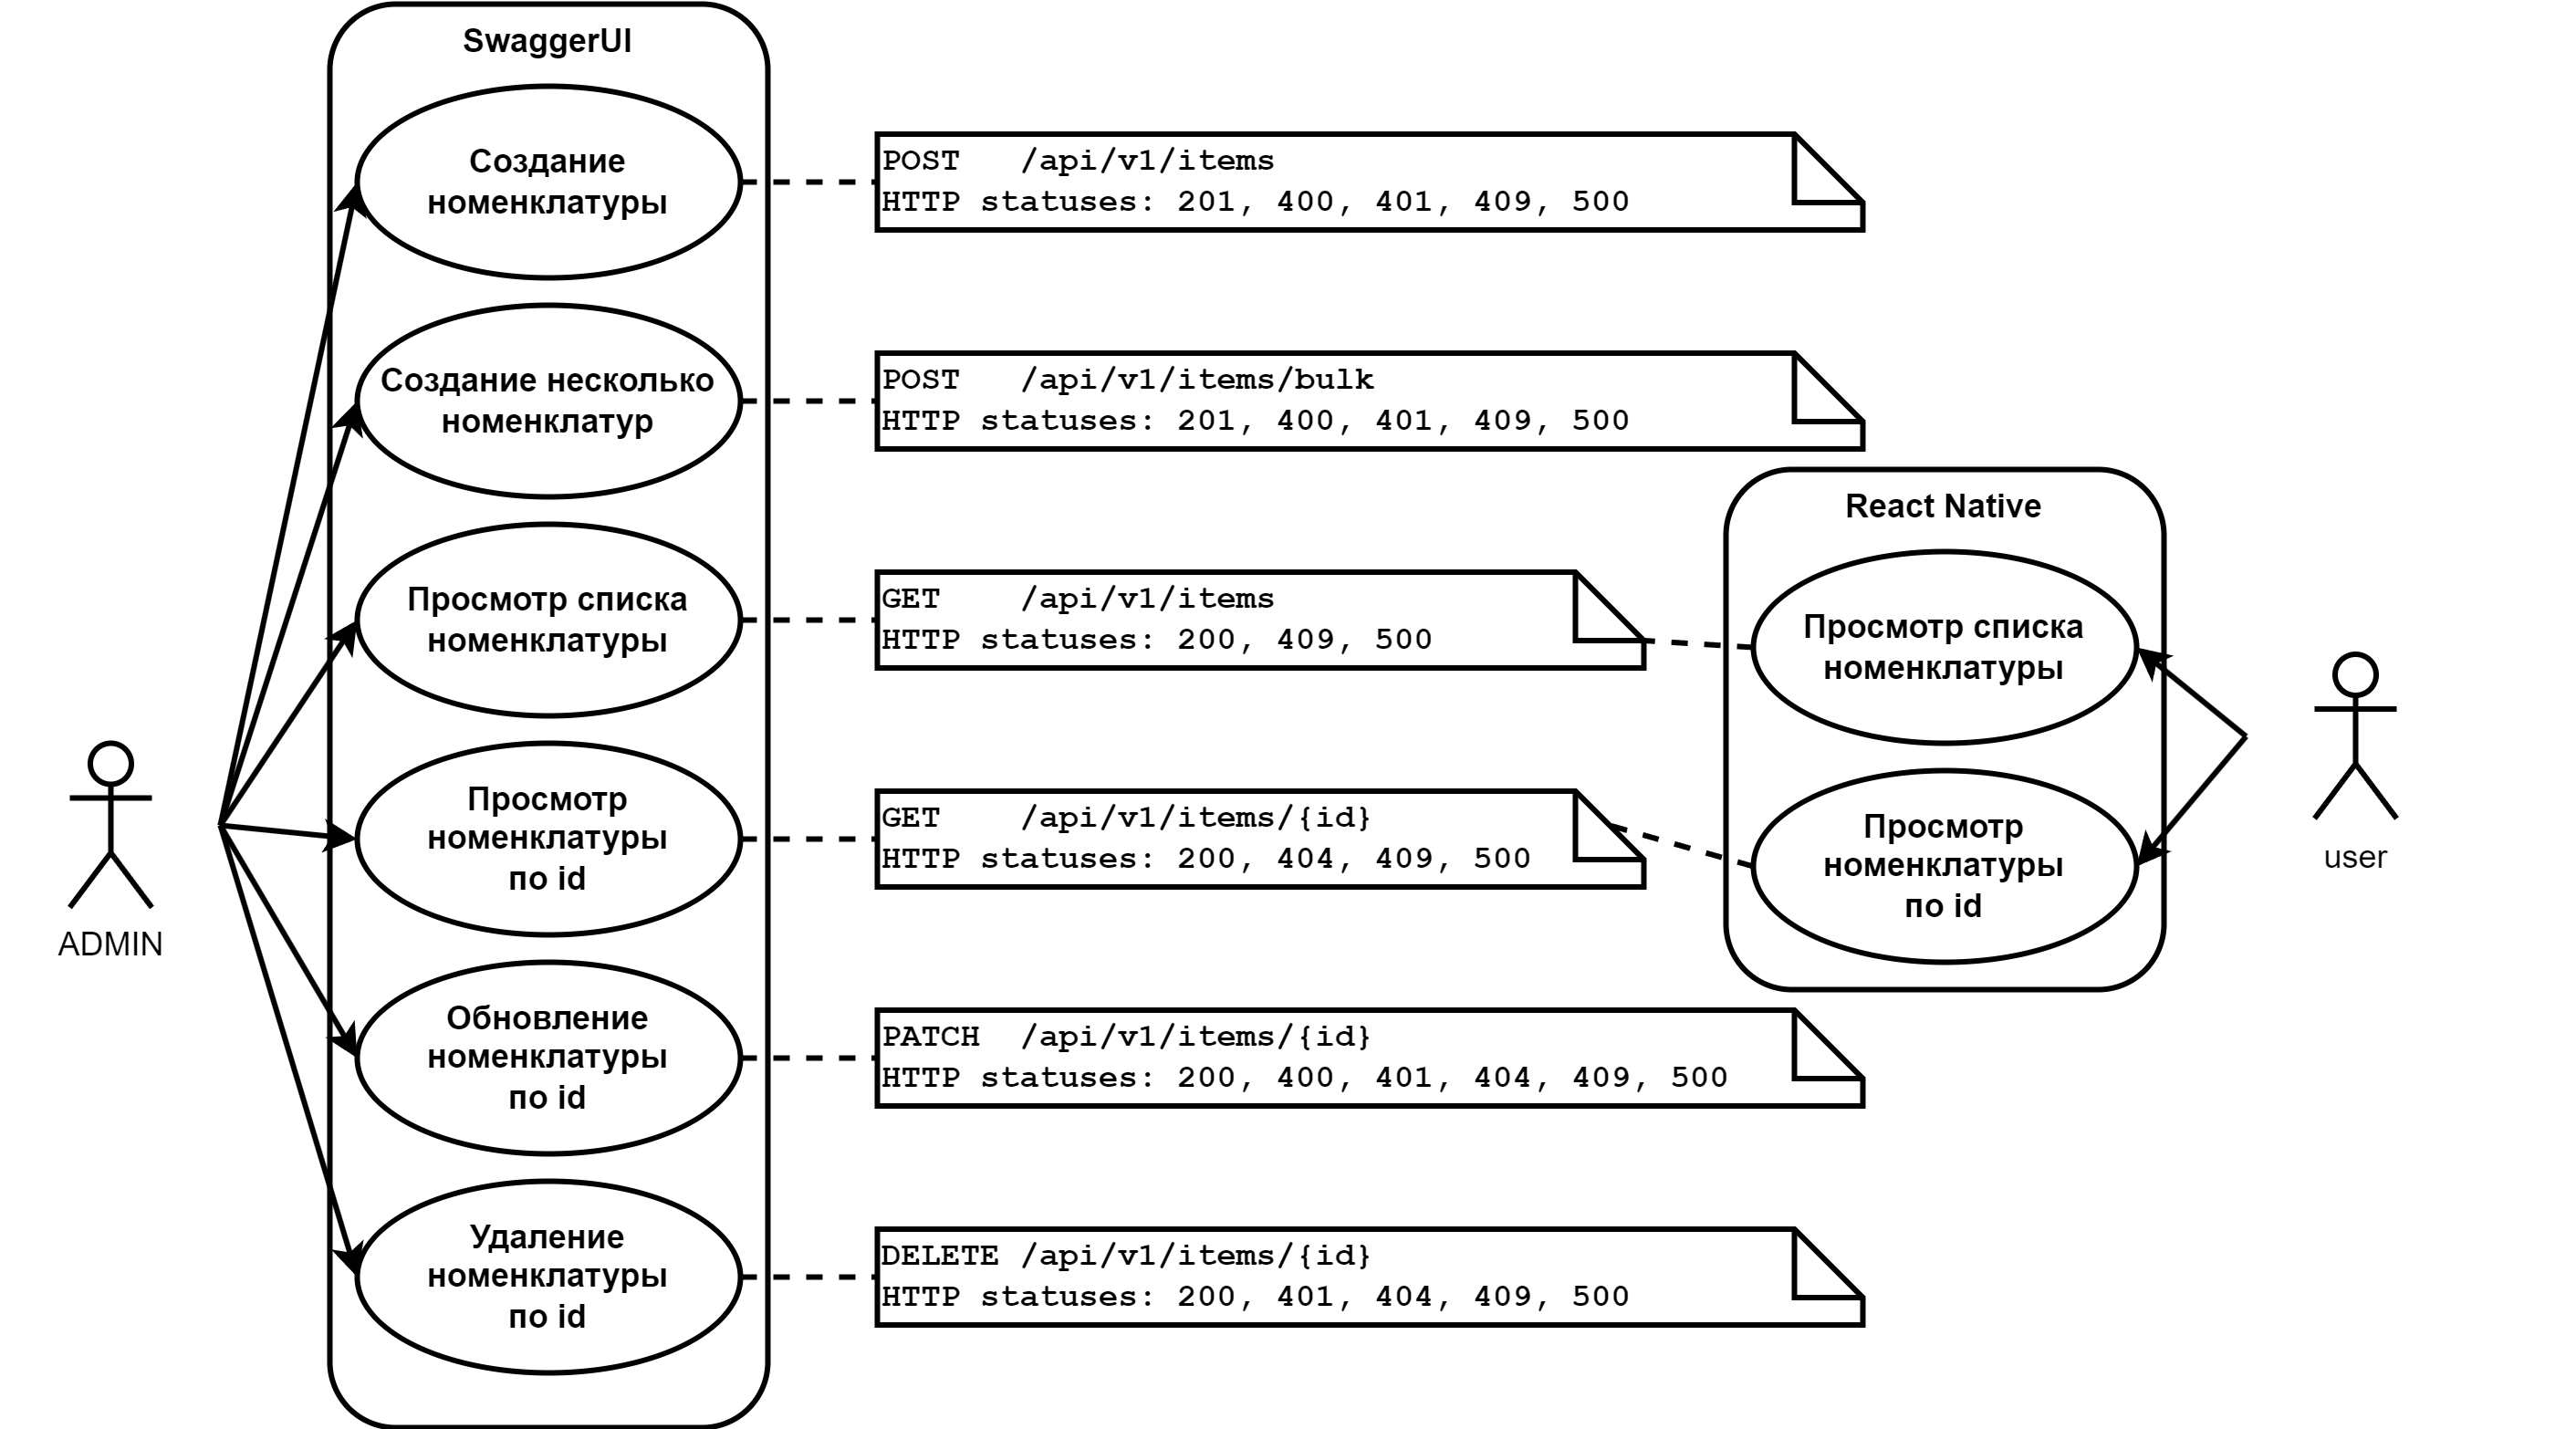
\includegraphics[width=17cm]
    {images/UML/UML_precedent_items.png}

    \caption{Диаграмма прецедентов для манипуляции с номенклутурой}

    \label{fig:UML_precedent_items}
\end{figure}

% = = = = = = = =

\subparagraph{Прецедент <<Создание категории номенклатуры>>} \hspace{0pt}

\underline{Назначение}: записать категорию номенклатуры в БД.

\underline{Исполнители}: администратор, браузер.

\underline{Эндпоинт}: POST /api/v1/item-categories.

\underline{Предусловие}: у пользователя есть токен доступа и роль admin.

\underline{Основной поток событий}: HTTP статус 201 (Created) - администратор создал категорию номенклатуры в БД. 

\underline{Альтернативный поток событий}:
HTTP статус 500 (Internal Server Error) - что-то пошло не так на сервере.

Диаграмма прецедентов изображены на рис.~\ref{fig:UML_precedent_item_categories}.

% = = = = = = = =

\subparagraph{Прецедент <<Просмотр списка категорий номенклатуры>>} \hspace{0pt}

\underline{Назначение}: просмотр списка категорий номенклатуры.

\underline{Исполнители}: мобильный клиент, браузер.

\underline{Эндпоинт}: GET /api/v1/item-categories.

% \underline{Предусловие}: 

\underline{Основной поток событий}: HTTP статус 200 (OK) - пользователь получил список номенклатуры. 

\underline{Альтернативный поток событий}:
HTTP статус 500 (Internal Server Error) - что-то пошло не так на сервере.

Диаграмма прецедентов изображены на рис.~\ref{fig:UML_precedent_item_categories}.

% = = = = = = = =

\subparagraph{Прецедент <<Просмотр категории номенклатуры по id>>} \hspace{0pt}

\underline{Назначение}: просмотр определённой номенклатуры.

\underline{Исполнители}: мобильный клиент, браузер.

\underline{Эндпоинт}: GET /api/v1/item-categories/:id.

% \underline{Предусловие}: 

\underline{Основной поток событий}: HTTP статус 200 (OK) - пользователь получил данные категории номенклатуры по id. 

\underline{Альтернативный поток событий}:

\begin{itemize}
    \item HTTP статус 404 (Not Found) - данные о категории номенклатуры по указанному id не найдены;
    \item HTTP статус 500 (Internal Server Error) - что-то пошло не так на сервере.
\end{itemize}

Диаграмма прецедентов изображены на рис.~\ref{fig:UML_precedent_item_categories}.

% = = = = = = = =

\subparagraph{Прецедент <<Обновление категории номенклатуры по id>>} \hspace{0pt}

\underline{Назначение}: обновить данные о номенклатуре по id.

\underline{Исполнители}: администратор, браузер.

\underline{Эндпоинт}: PATCH /api/v1/item-categories/:id.

\underline{Предусловие}: у пользователя есть токен доступа и роль admin.

\underline{Основной поток событий}: HTTP статус 200 (OK) - администратор обновил данные о категории номенклатуры по id. 

\underline{Альтернативный поток событий}:

\begin{itemize}
    \item HTTP статус 404 (Not Found) - данные о категории номенклатура по id не найдены;
    \item HTTP статус 500 (Internal Server Error) - что-то пошло не так на сервере.
\end{itemize}

Диаграмма прецедентов изображены на рис.~\ref{fig:UML_precedent_item_categories}.

% = = = = = = = =

\subparagraph{Прецедент <<Удаление категории номенклатуры по id>>} \hspace{0pt}

\underline{Назначение}: удалить данные о категории номенклатуры по id.

\underline{Исполнители}: администратор, браузер.

\underline{Эндпоинт}: DELETE /api/v1/item-categories/:id.

\underline{Предусловие}: у пользователя есть токен доступа и роль admin.

\underline{Основной поток событий}: HTTP статус 200 (OK) - администратор обновил данные о номенклатуре по uuid. 

\underline{Альтернативный поток событий}:

\begin{itemize}
    \item HTTP статус 404 (Not Found) - данные о категории номенклатуры по id не найдены;
    \item HTTP статус 500 (Internal Server Error) - что-то пошло не так на сервере.
\end{itemize}

Диаграмма прецедентов изображены на рис.~\ref{fig:UML_precedent_item_categories}.

% = = = = = = = =

\begin{figure}[!htb]
    \centering

    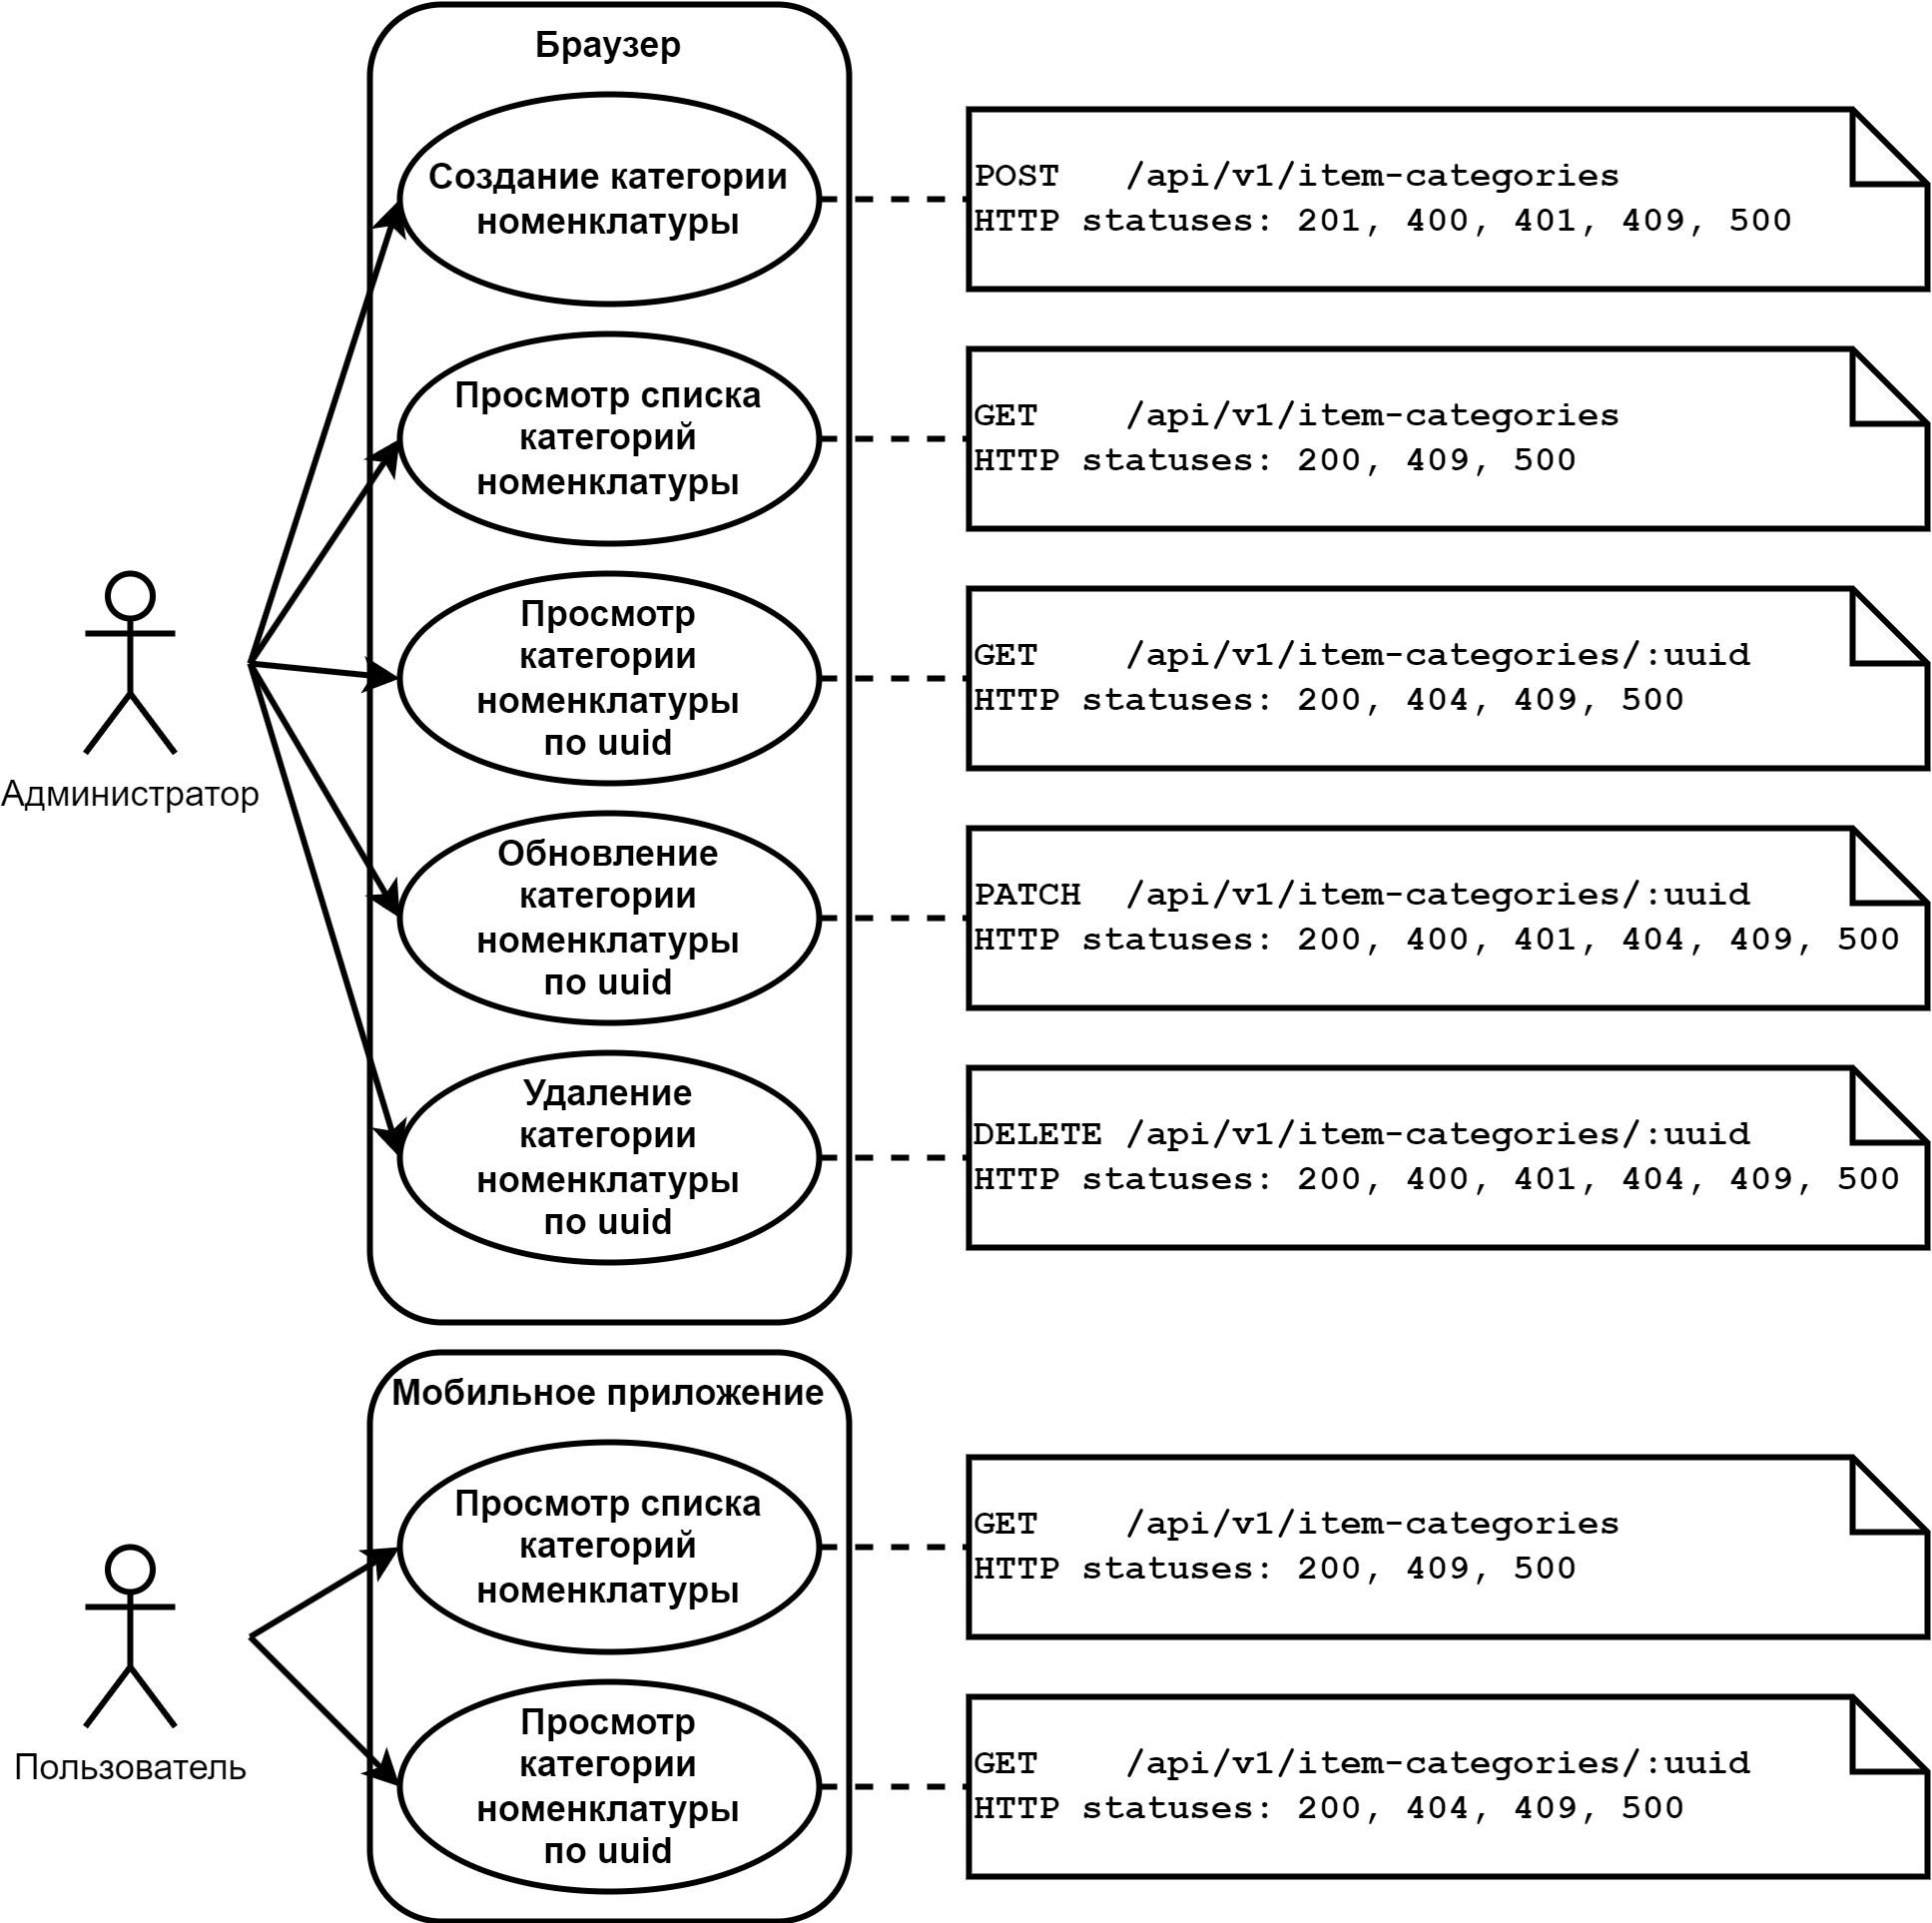
\includegraphics[width=15cm]
    {images/UML/UML_precedent_item_categories.png}

    \caption{Диаграмма прецедентов для манипуляции с категориями номенклатуры}

    \label{fig:UML_precedent_item_categories}
\end{figure}

% = = = = = = = =

\subparagraph{Прецедент <<Создание помощника (контакта рабочего)>>} \hspace{0pt}

\underline{Назначение}: создать контакт работника, который будет доступен в интернете, чтобы с ним связаться.

\underline{Исполнители}: администратор, браузер.

\underline{Эндпоинт}: POST /api/v1/helpers.

\underline{Предусловие}: у пользователя есть токен доступа и роль admin.

\underline{Основной поток событий}: HTTP статус 201 (Created) - администратор создал помощника в БД. 

\underline{Альтернативный поток событий}:
HTTP статус 500 (Internal Server Error) - что-то пошло не так на сервере.

Диаграмма прецедентов изображены на рис.~\ref{fig:UML_precedent_helpres}.

% = = = = = = = =

\subparagraph{Прецедент <<Просмотр списка помощников>>} \hspace{0pt}

\underline{Назначение}: просмотр списка помощников.

\underline{Исполнители}: мобильный клиент, браузер.

\underline{Эндпоинт}: GET /api/v1/helpers.

% \underline{Предусловие}: 

\underline{Основной поток событий}: HTTP статус 200 (OK) - пользователь получил список помощников. 

\underline{Альтернативный поток событий}:
HTTP статус 500 (Internal Server Error) - что-то пошло не так на сервере.

Диаграмма прецедентов изображены на рис.~\ref{fig:UML_precedent_helpres}.

% = = = = = = = =

\subparagraph{Прецедент <<Просмотр помощника по id>>} \hspace{0pt}

\underline{Назначение}: просмотр данных определённого помощника.

\underline{Исполнители}: мобильный клиент, браузер.

\underline{Эндпоинт}: GET /api/v1/helpers/:id.

% \underline{Предусловие}: 

\underline{Основной поток событий}: HTTP статус 200 (OK) - пользователь получил данные помощника по id. 

\underline{Альтернативный поток событий}:

\begin{itemize}
    \item HTTP статус 404 (Not Found) - данные о помощнике по указанному id не найдены;
    \item HTTP статус 500 (Internal Server Error) - что-то пошло не так на сервере.
\end{itemize}

Диаграмма прецедентов изображены на рис.~\ref{fig:UML_precedent_helpres}.

% = = = = = = = =

\subparagraph{Прецедент <<Обновление помощника по id>>} \hspace{0pt}

\underline{Назначение}: обновить данные о помощнике по id.

\underline{Исполнители}: администратор, браузер.

\underline{Эндпоинт}: PATCH /api/v1/helper/:id.

\underline{Предусловие}: у пользователя есть токен доступа и роль admin.

\underline{Основной поток событий}: HTTP статус 200 (OK) - администратор обновил данные о помощнике по id. 

\underline{Альтернативный поток событий}:

\begin{itemize}
    \item HTTP статус 404 (Not Found) - данные о помощнике по id не найдены;
    \item HTTP статус 500 (Internal Server Error) - что-то пошло не так на сервере.
\end{itemize}

Диаграмма прецедентов изображены на рис.~\ref{fig:UML_precedent_helpres}.

% = = = = = = = =

\subparagraph{Прецедент <<Удаление помощника по id>>} \hspace{0pt}

\underline{Назначение}: удалить данные о помощнике по id.

\underline{Исполнители}: администратор, браузер.

\underline{Эндпоинт}: DELETE /api/v1/item-categories/:id.

\underline{Предусловие}: у пользователя есть токен доступа и роль admin.

\underline{Основной поток событий}: HTTP статус 200 (OK) - администратор удалил данные о помощнике по id. 

\underline{Альтернативный поток событий}:

\begin{itemize}
    \item HTTP статус 404 (Not Found) - данные о помощнике по id не найдены;
    \item HTTP статус 500 (Internal Server Error) - что-то пошло не так на сервере.
\end{itemize}

Диаграмма прецедентов изображены на рис.~\ref{fig:UML_precedent_helpres}.

% = = = = = = = =

\begin{figure}[!p]
    \centering

    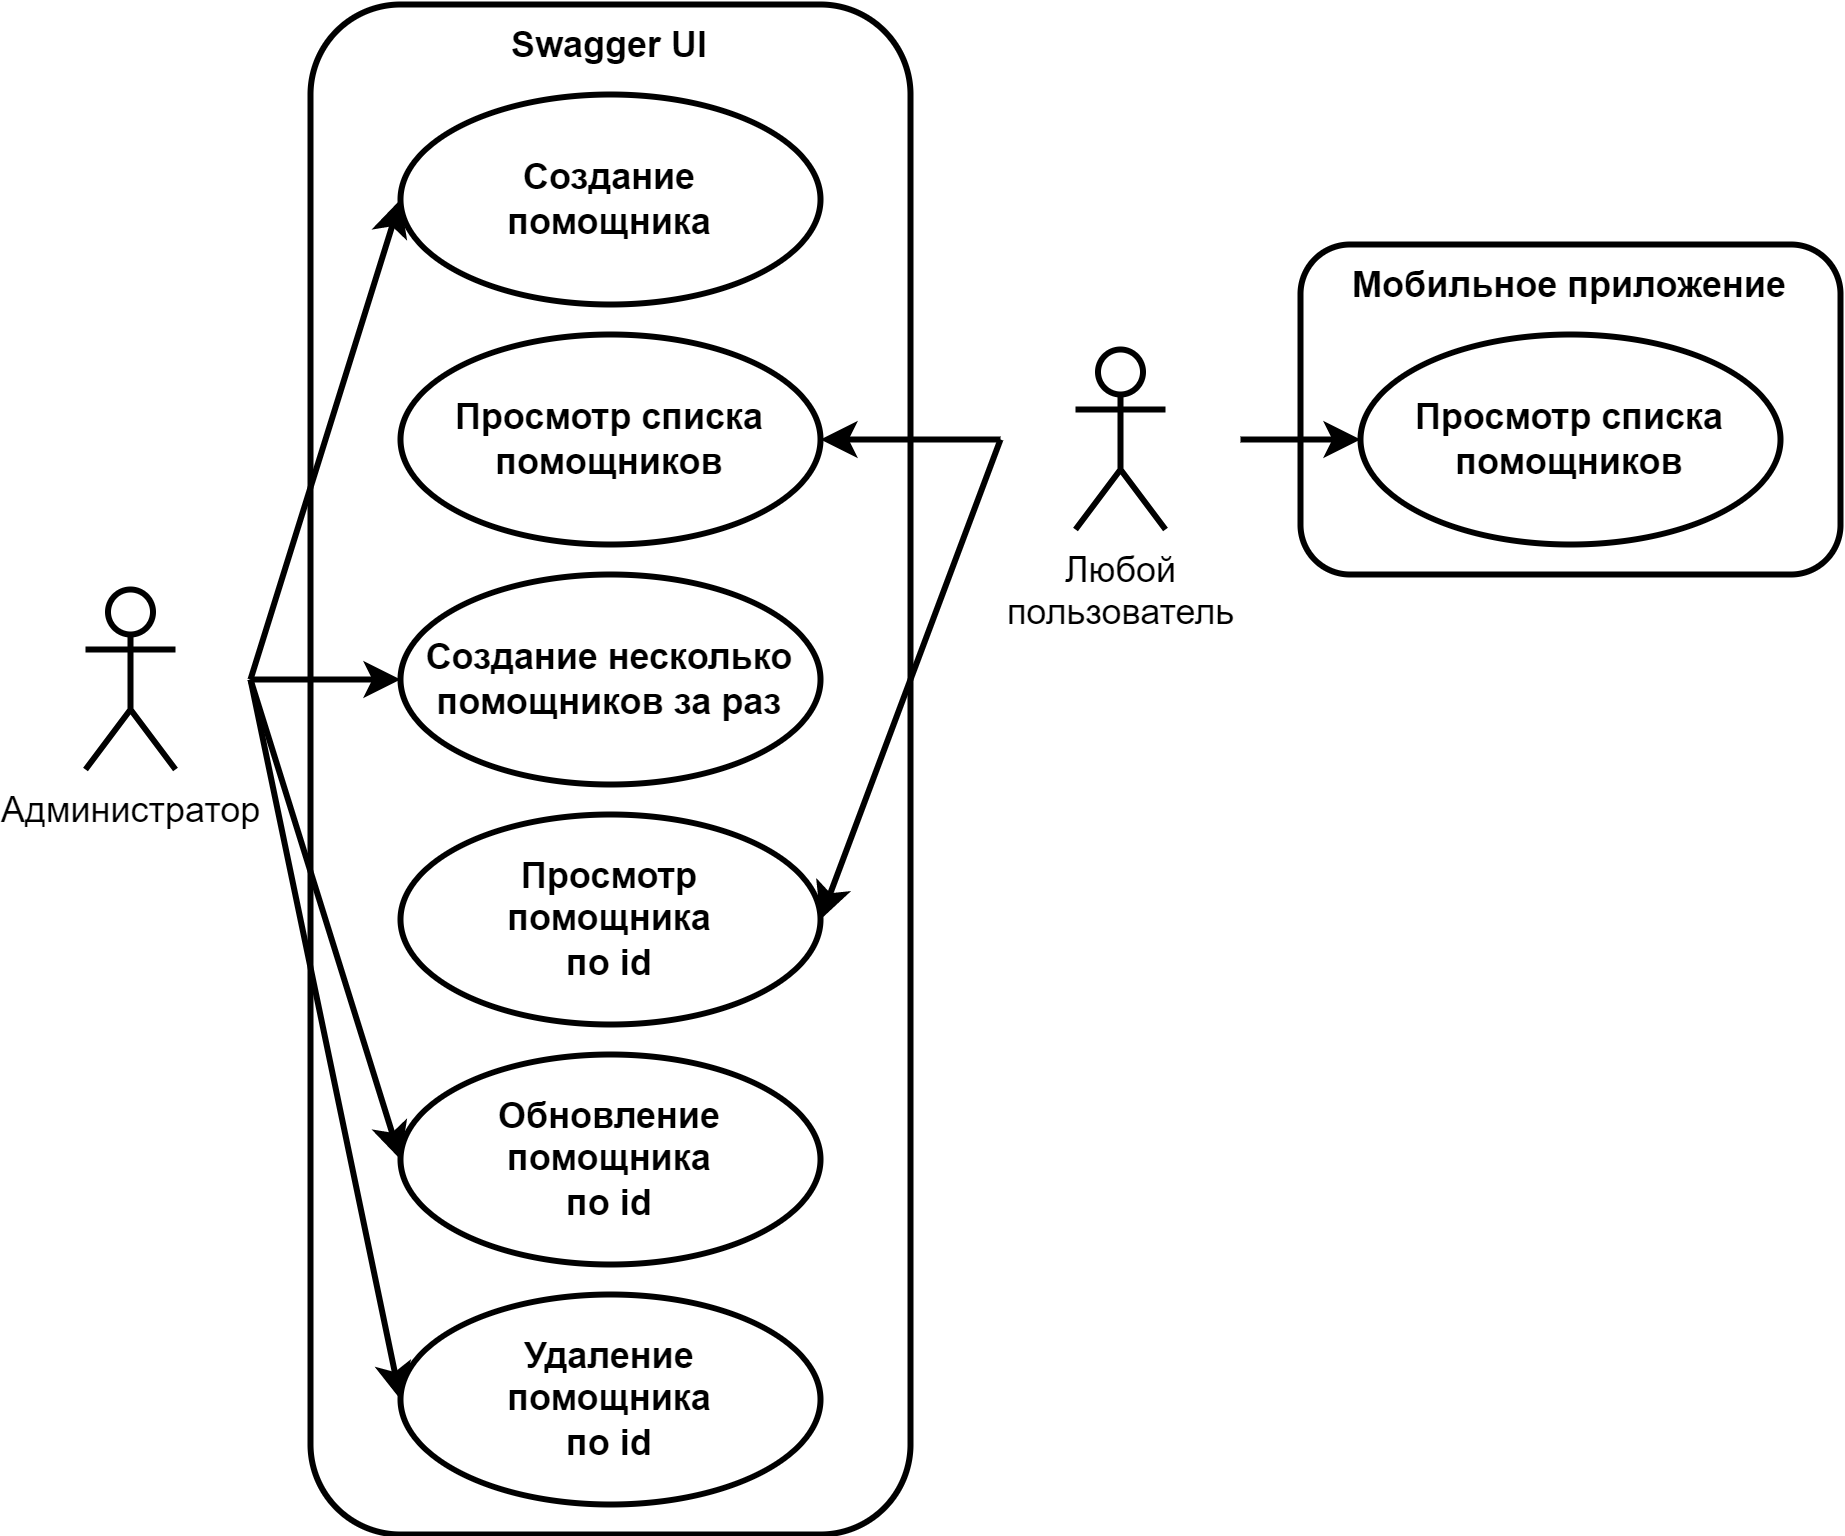
\includegraphics[height=11cm]
    {images/UML/UML_precedent_helpres.png}

    \caption{Диаграмма прецедентов для манипуляции с помощниками}

    \label{fig:UML_precedent_helpres}
\end{figure}

% = = = = = = = =

\subparagraph{Прецедент <<Создание статьи>>} \hspace{0pt}

\underline{Назначение}: создать статью для сайта.

\underline{Исполнители}: администратор, браузер.

\underline{Эндпоинт}: POST /api/v1/articles.

\underline{Предусловие}: у пользователя есть токен доступа и роль admin.

\underline{Основной поток событий}: HTTP статус 201 (Created) - администратор создал статью для сайта в БД. 

\underline{Альтернативный поток событий}:
HTTP статус 500 (Internal Server Error) - что-то пошло не так на сервере.

Диаграмма прецедентов изображены на рис.~\ref{fig:UML_precedent_articles}.

% = = = = = = = =

\subparagraph{Прецедент <<Просмотр списка статей>>} \hspace{0pt}

\underline{Назначение}: просмотр списка статей для сайта.

\underline{Исполнители}: мобильный клиент, браузер.

\underline{Эндпоинт}: GET /api/v1/articles.

% \underline{Предусловие}: 

\underline{Основной поток событий}: HTTP статус 200 (OK) - пользователь получил список статей. 

\underline{Альтернативный поток событий}:
HTTP статус 500 (Internal Server Error) - что-то пошло не так на сервере.

Диаграмма прецедентов изображены на рис.~\ref{fig:UML_precedent_articles}.

% = = = = = = = =

\subparagraph{Прецедент <<Просмотр статьи по urlSegment>>} \hspace{0pt}

\underline{Назначение}: просмотр данных статьи.

\underline{Исполнители}: мобильный клиент, браузер.

\underline{Эндпоинт}: GET /api/v1/articles/:urlSegment.

% \underline{Предусловие}: 

\underline{Основной поток событий}: HTTP статус 200 (OK) - пользователь получил статью по urlSegment. 

\underline{Альтернативный поток событий}:

\begin{itemize}
    \item HTTP статус 404 (Not Found) - данные о статье urlSegment не найдены;
    \item HTTP статус 500 (Internal Server Error) - что-то пошло не так на сервере.
\end{itemize}

Диаграмма прецедентов изображены на рис.~\ref{fig:UML_precedent_articles}.

% = = = = = = = =

\subparagraph{Прецедент <<Обновление статью по uuid>>} \hspace{0pt}

\underline{Назначение}: обновить данные о стаье по uuid.

\underline{Исполнители}: администратор, браузер.

\underline{Эндпоинт}: PATCH /api/v1/articles/:uuid.

\underline{Предусловие}: у пользователя есть токен доступа и роль admin.

\underline{Основной поток событий}: HTTP статус 200 (OK) - администратор обновил данные о статье по uuid. 

\underline{Альтернативный поток событий}:

\begin{itemize}
    \item HTTP статус 404 (Not Found) - данные о статье по uuid не найдены;
    \item HTTP статус 500 (Internal Server Error) - что-то пошло не так на сервере.
\end{itemize}

Диаграмма прецедентов изображены на рис.~\ref{fig:UML_precedent_articles}.

% = = = = = = = =

\subparagraph{Прецедент <<Удаление статьи по id>>} \hspace{0pt}

\underline{Назначение}: удалить данные о статье по id.

\underline{Исполнители}: администратор, браузер.

\underline{Эндпоинт}: DELETE /api/v1/articles/:uuid.

\underline{Предусловие}: у пользователя есть токен доступа и роль admin.

\underline{Основной поток событий}: HTTP статус 200 (OK) - администратор удалил данные о статье по uuid. 

\underline{Альтернативный поток событий}:

\begin{itemize}
    \item HTTP статус 404 (Not Found) - данные о статье по uuid не найдены;
    \item HTTP статус 500 (Internal Server Error) - что-то пошло не так на сервере.
\end{itemize}

Диаграмма прецедентов изображены на рис.~\ref{fig:UML_precedent_articles}.

% = = = = = = = =

\begin{figure}[!p]
    \centering

    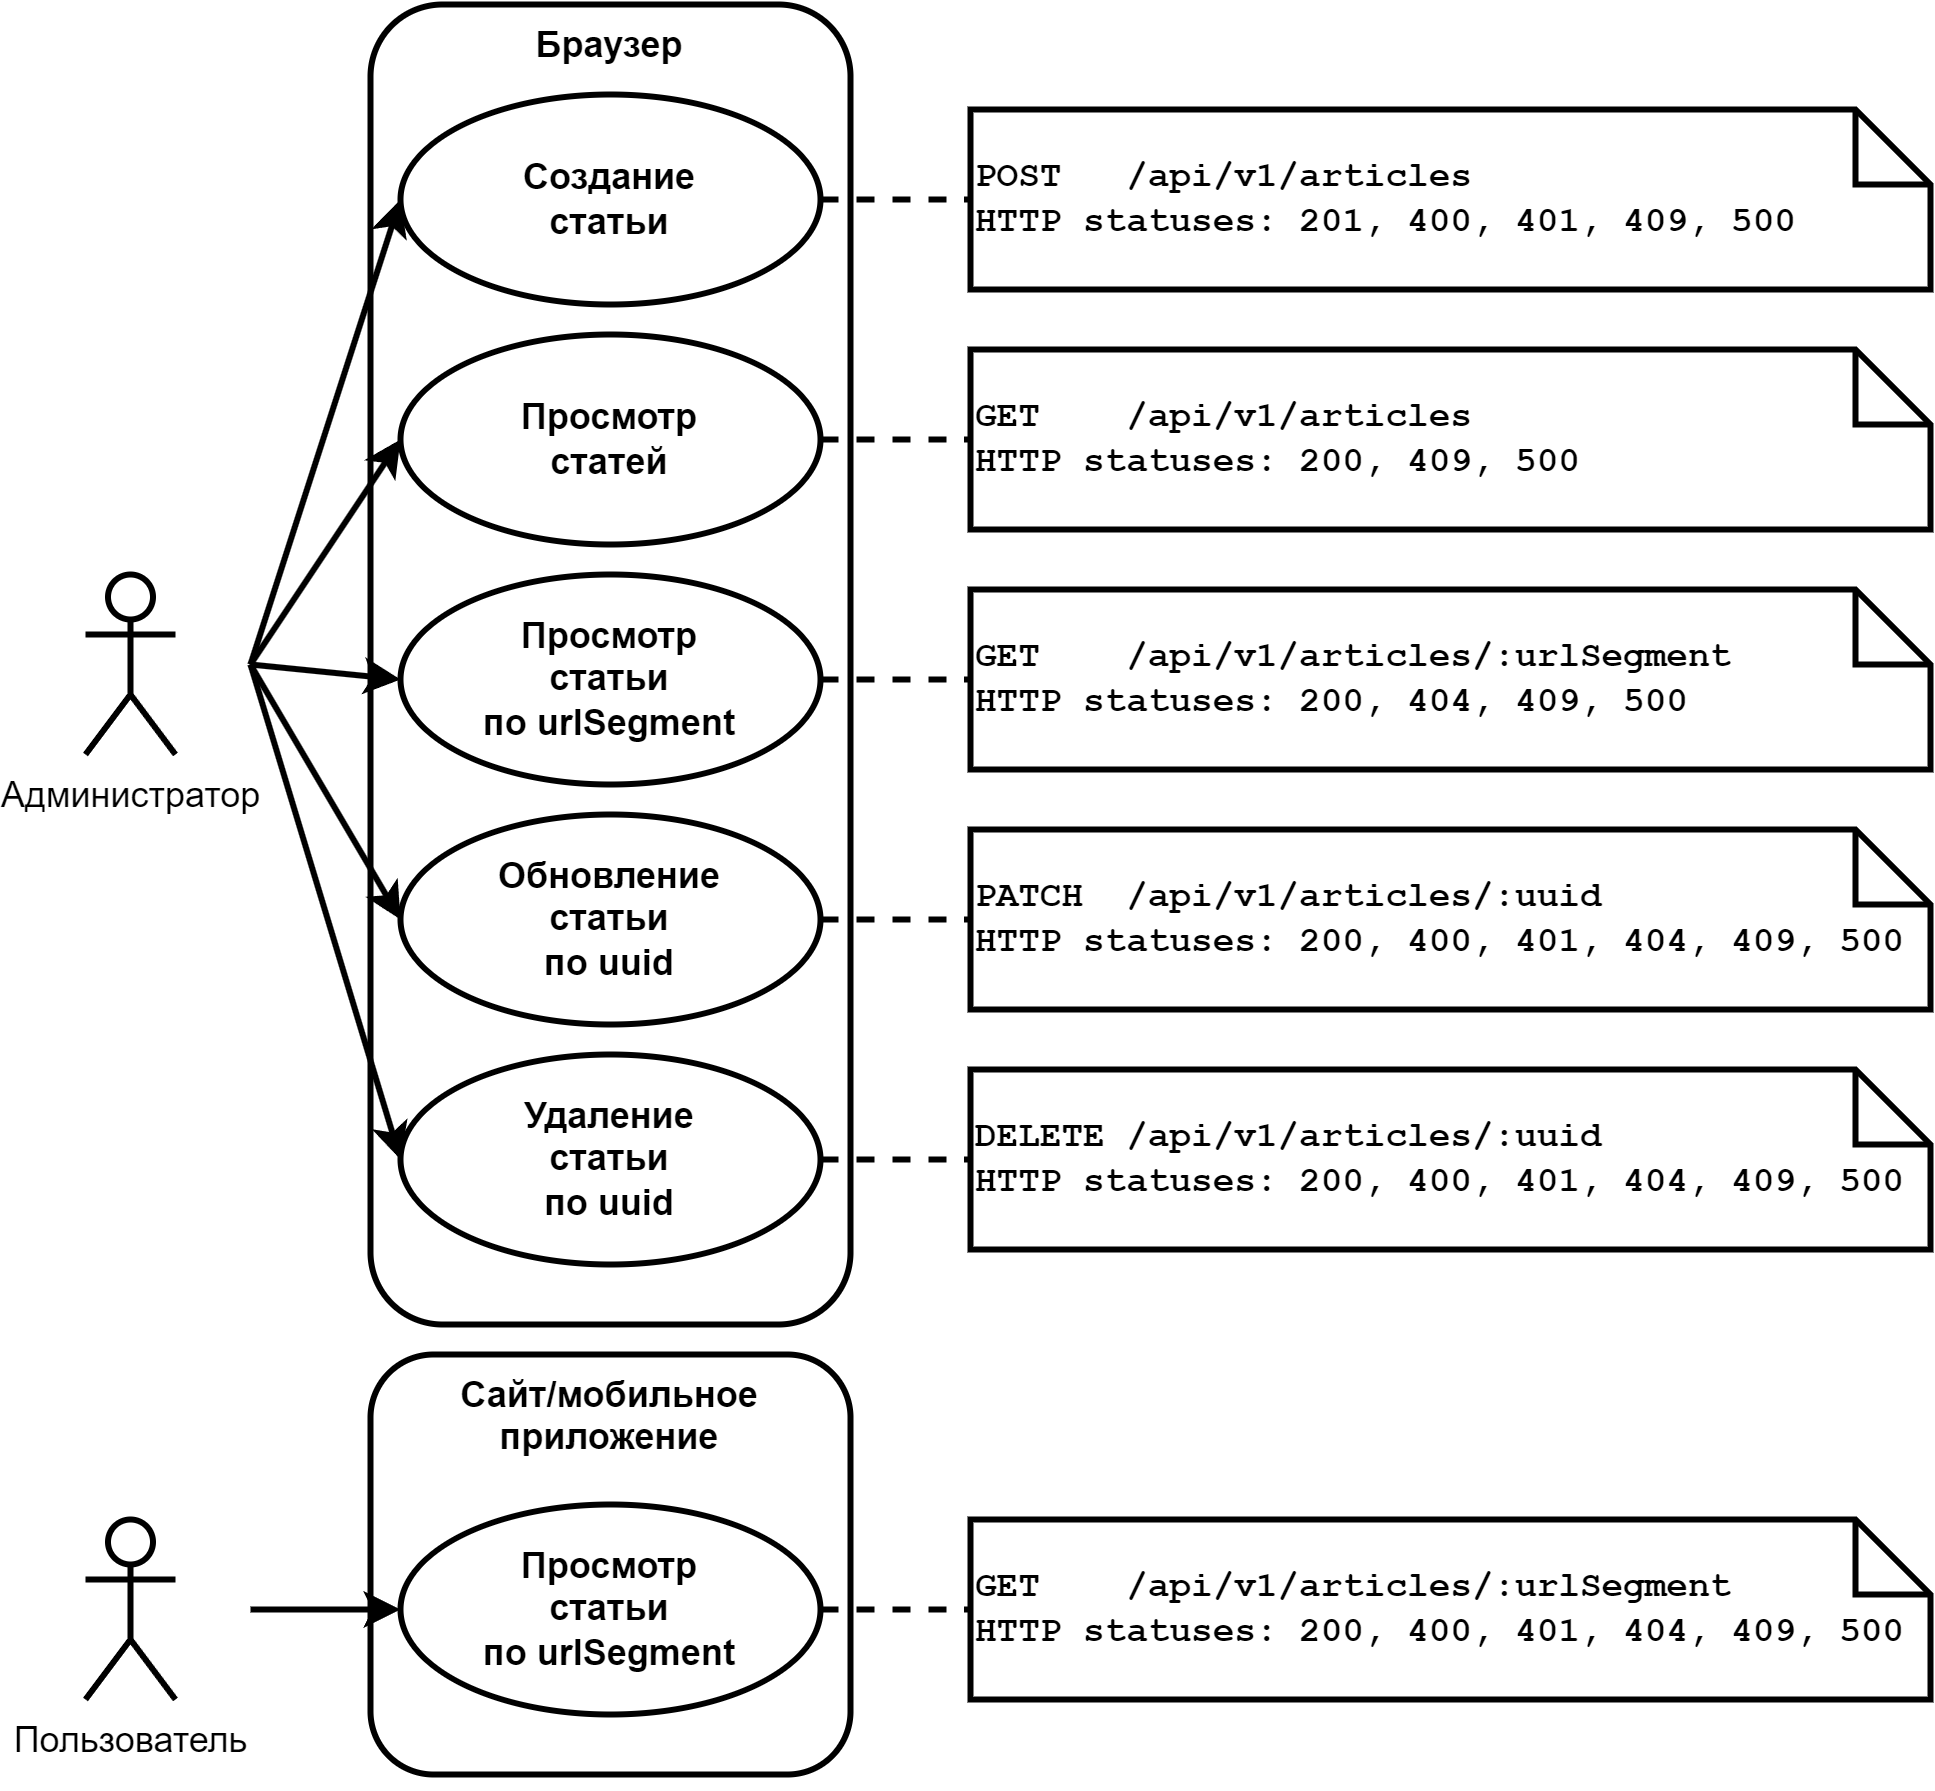
\includegraphics[height=11cm]
    {images/UML/UML_precedent_articles.png}

    \caption{Диаграмма прецедентов для манипуляции со статьями}

    \label{fig:UML_precedent_articles}
\end{figure}

% = = = = = = = =

% \subparagraph{Прецедент <<Просмотр пользователей>>} \hspace{0pt}

% \underline{Назначение}: просмотр списка пользователей.

% \underline{Исполнители}: браузер.

% \underline{Эндпоинт}: GET /api/v1/users.

% \underline{Предусловие}: у пользователя есть токен доступа и роль admin.

% \underline{Основной поток событий}: HTTP статус 200 (OK) - администратор получил список пользователей. 

% \underline{Альтернативный поток событий}:
% HTTP статус 500 (Internal Server Error) - что-то пошло не так на сервере.

% Диаграмма прецедентов изображены на рис.~\ref{fig:UML_precedent_users}.

% = = = = = = = =

% \subparagraph{Прецедент <<Просмотр пользователя по id>>} \hspace{0pt}

% \underline{Назначение}: просмотр данных статьи.

% \underline{Исполнители}: браузер.

% \underline{Эндпоинт}: GET /api/v1/users/:id.

% \underline{Предусловие}: у пользователя есть токен доступа и роль admin.

% \underline{Основной поток событий}: HTTP статус 200 (OK) - администратор получил данные пользователя по id. 

% \underline{Альтернативный поток событий}:

% \begin{itemize}
%     \item HTTP статус 404 (Not Found) - данные о пользователе по id не найдены;
%     \item HTTP статус 500 (Internal Server Error) - что-то пошло не так на сервере.
% \end{itemize}

% Диаграмма прецедентов изображены на рис.~\ref{fig:UML_precedent_users}.

% = = = = = = = =

% \subparagraph{Прецедент <<Блокировка пользователя>>} \hspace{0pt}

% \underline{Назначение}: блокировка пользователя.

% \underline{Исполнители}: браузер.

% \underline{Эндпоинт}: PATCH /api/v1/users/:id/ban.

% \underline{Предусловие}: у пользователя есть токен доступа и роль admin.

% \underline{Основной поток событий}: HTTP статус 200 (OK) - администратор заблокировал пользователя по id. 

% \underline{Альтернативный поток событий}:

% \begin{itemize}
%     \item HTTP статус 404 (Not Found) - пользователь по id не найден;
%     \item HTTP статус 500 (Internal Server Error) - что-то пошло не так на сервере.
% \end{itemize}

% Диаграмма прецедентов изображены на рис.~\ref{fig:UML_precedent_users}.

% = = = = = = = =

% \subparagraph{Прецедент <<Разблокировка пользователя>>} \hspace{0pt}

% \underline{Назначение}: разблокировка пользователя.

% \underline{Исполнители}: браузер.

% \underline{Эндпоинт}: PATCH /api/v1/users/:id/unban.

% \underline{Предусловие}: у пользователя есть токен доступа и роль admin.

% \underline{Основной поток событий}: HTTP статус 200 (OK) - администратор разблокировал пользователя по id. 

% \underline{Альтернативный поток событий}:

% \begin{itemize}
%     \item HTTP статус 404 (Not Found) - пользователь по id не найден;
%     \item HTTP статус 500 (Internal Server Error) - что-то пошло не так на сервере.
% \end{itemize}

% Диаграмма прецедентов изображены на рис.~\ref{fig:UML_precedent_users}.

% = = = = = = = =

% \begin{figure}[!htb]
%     \centering

%     \includegraphics[width=12cm]
%     {images/UML/UML_precedent_users.png}

%     \caption{Диаграмма прецедентов для манипуляции с пользователями}

%     \label{fig:UML_precedent_users}
% \end{figure}

% = = = = = = = =

\subsection*{Диграмма последовательностей}

% UML диаграмма последовательности (Sequence diagram) - это диаграмма, которая отображает взаимодействие между объектами или компонентами в системе
% в виде последовательности сообщений, которые передаются между ними.

% Диаграмма последовательностей спроектирована в draw.io \cite{drawio} и изображена на рис.~\ref{fig:UML_sequence_diagram}.

% UML диаграмма последовательности позволяет представить взаимодействие между объектами в форме временной последовательности,
% показывая, как каждый объект взаимодействует с другими и когда это происходит. Объекты изображаются в виде вертикальных линий (жизненных линий),
% а сообщения между объектами отображаются в виде стрелок, которые указывают направление передачи информации.

UML (Unified Modeling Language) диаграмма последовательностей (англ. sequence diagram) отображает
взаимодействие объектов или компонентов в виде вертикальных линий, известных как <<жизненные линии>>.
По мере выполнения определенных действий или вызова методов,
сообщения и события передаются между участниками системы,
что отображается в виде стрелок, соединяющих соответствующие жизненные линии.
Это позволяет легко проследить порядок выполнения операций и взаимодействие между различными элементами системы.

На рисунке~\ref{fig:UML_sequence_diagram} представлена диаграмма последовательностей,
демонстрирующая взаимодействие между мобильным приложением, серверной частью и базой данных.

\begin{figure}[!htb]
    \centering

    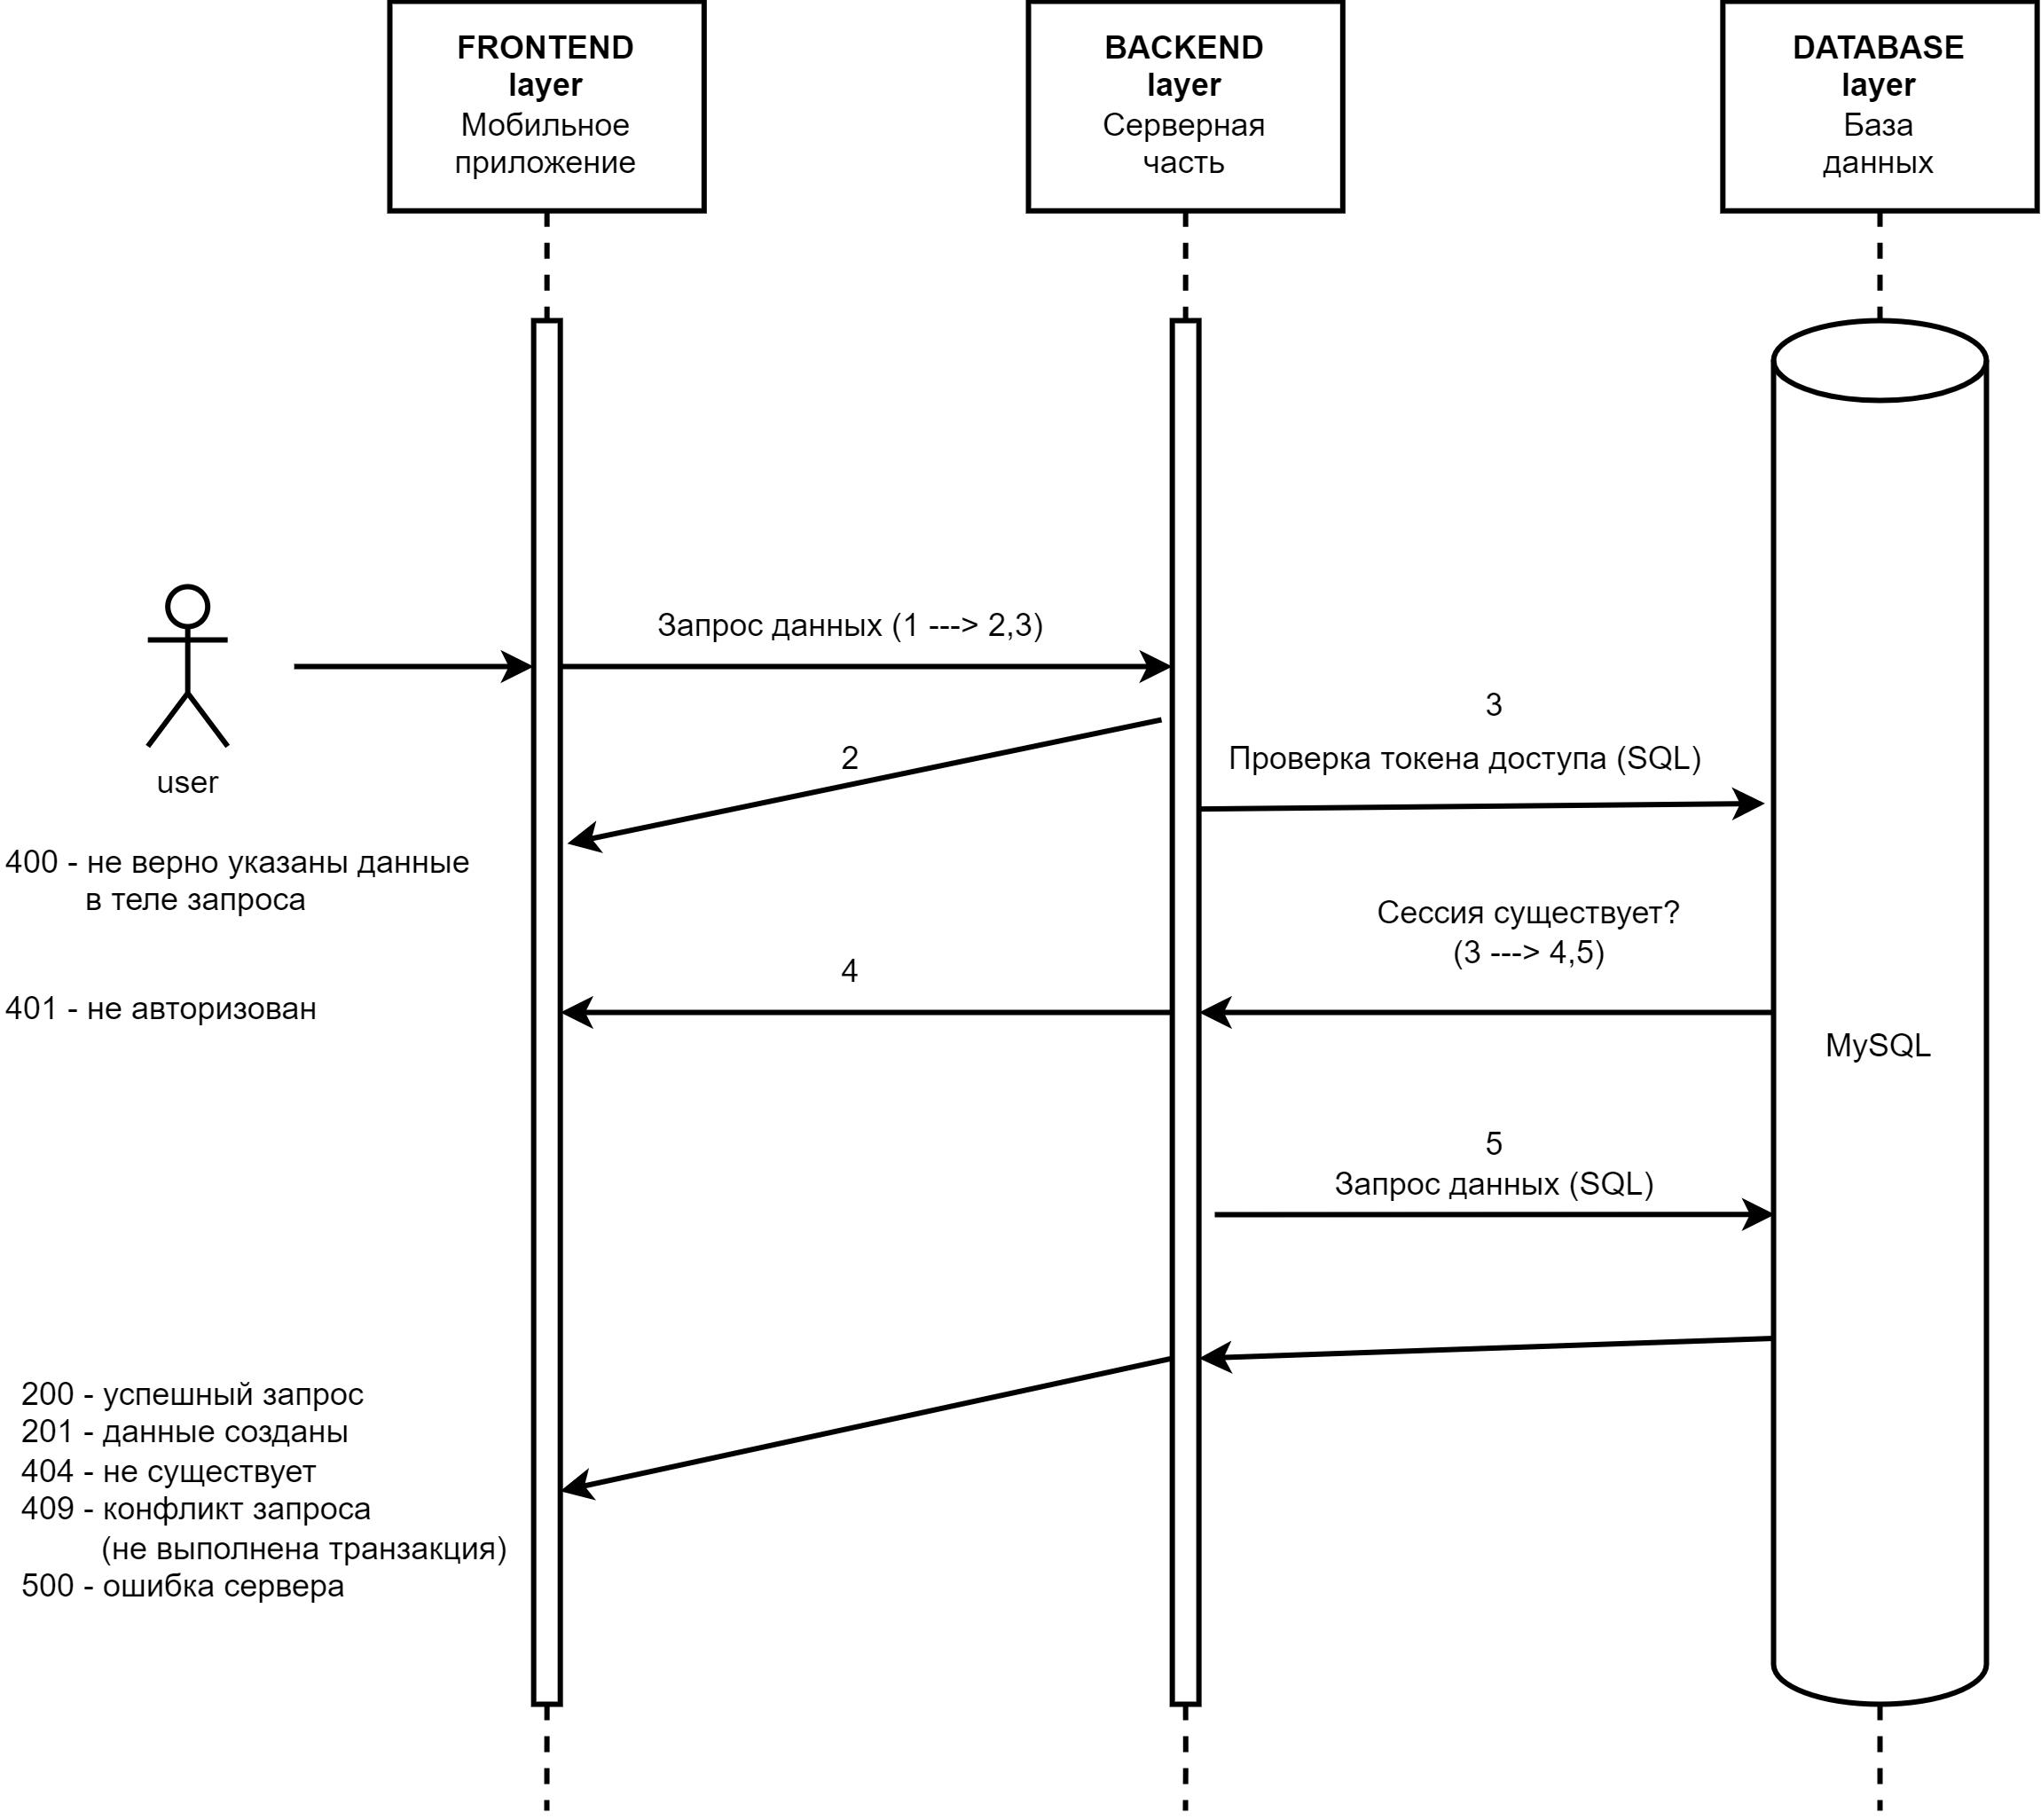
\includegraphics[width=14cm]
    {images/UML/sequence/sequence.png}

    \caption{Диаграмма последовательностей}

    \label{fig:UML_sequence_diagram}
\end{figure}

\subsection{Участники системы и их взаимодействие}

Эндпоинт - конечная точка веб-приложения или API для доступа к ресурсам или операций.
Он представляет собой URL-адрес, через который можно отправлять запросы и получать ответы от сервера.

HTTP-статусы - числовые коды, возвращаемые в ответ на HTTP-запросы,
чтобы указать состояние выполнения запроса или передать дополнительную информацию о результате операции.
% Каждый статус имеет свою семантику, например, 200 (OK) указывает на успешное выполнение запроса,
% а 404 (Not Found) означает, что запрашиваемый ресурс не найден.

% Методы - операции или действия, выполняемые с использованием HTTP-протокола.

Методы в контексте HTTP-протокола представляют собой определенные действия или операции,
которые могут быть выполнены для обмена информацией между клиентом и сервером.
Они определяют тип запроса и указывают на необходимые действия, такие как получение данных (GET), отправка данных (POST), обновление данных (PUT), удаление данных (DELETE) и другие.

Перечень HTTP запросов для разрабатываемого приложения и соответствующие им роли приведены в таблице~\ref{tabl:swagger}.

\begin{sidewaystable}
    \small
    \caption{Участники системы и их взаимодействие} \label{tabl:swagger}

    \begin{tabular}{|p{1cm}|p{1cm}|p{8.5cm}|p{4.8cm}|p{8cm}|}
        \hline
        \multicolumn{1}{|c|}{Роль}
        & \multicolumn{1}{c|}{Метод}
        & \multicolumn{1}{c|}{Эндпоинт}
        & \multicolumn{1}{c|}{HTTP статус}
        & \multicolumn{1}{c|}{Назначение}
        \\ \hline

        any & post & /api/v1/users & 200, 409, 500 & регистрация \\ \hline 
        admin & get & /api/v1/users & 200, 401, 404, 500 & получение списка пользователей \\ \hline 
        any & get & /api/v1/users/activate-account/\{token\} & 200, 404, 500 & активация аккаунта \\ \hline 
        user & patch & /api/v1/users/change-email & 200, 401, 409, 429, 500 & запрос на смену email \\ \hline 
        any & get & /api/v1/users/change-email/\{token\}/confirm & 200, 404, 500 & подтверждение смены email \\ \hline 
        any & get & /api/v1/users/change-email/\{token\}/delete & 200, 404, 500 & отмена смены email \\ \hline 
        any & post & /api/v1/users/forget-password & 200, 409, 500 & запросить логин и новый пароль \\ \hline 
        user & patch & /api/v1/users/change-password & 200, 401, 409, 500 & смена пароля \\ \hline
        admin & post & /api/v1/users/is-admin & 200, 401, 500 & проверка роли администратора\\ \hline 
        any & post & /api/v1/sessions & 201, 409, 500 & вход в аккаунт \\ \hline 
        user & get & /api/v1/sessions & 200, 401, 500 & получаем список сессий \\ \hline 
        any & patch & /api/v1/sessions & 200, 401, 500 & обновление токена доступа \\ \hline 
        user & delete & /api/v1/sessions & 200, 401, 500 & закрытие всех сессий \\ \hline 
        user & post & /api/v1/sessions/logout & 200, 500 & выход с аккаунта \\ \hline 
        user & delete & /api/v1/sessions/\{id\} & 200, 401, 500 & закрытие сессий по id \\ \hline 
        any & get & /api/v1/apk-versions & 200, 500 & получить последнию версию apk \\ \hline 
        admin & post & /api/v1/item-characteristics & 201, 400, 401, 409, 500 & создание характеристики \\ \hline 
        any & get & /api/v1/item-characteristics & 200, 500 & просмотр списка характеристик \\ \hline 
        admin & post & /api/v1/item-characteristics/bulk & 201, 400, 401, 409, 500 & добавление несколько записей за раз \\ \hline 
        admin & put & /api/v1/item-characteristics/bulk & 200, 400, 401, 409, 500 & обновление несколько записей за раз \\ \hline 
        any & get & /api/v1/item-characteristics/\{id\} & 200, 404, 500 & просмотр характеристики по id \\ \hline 
        admin & patch & /api/v1/item-characteristics/\{id\} & 200, 400, 401, 404, 409, 500 & обновление характеристики по id \\ \hline 
        admin & delete & /api/v1/item-characteristics/\{id\} & 200, 401, 404, 500 & удаление характеристики по id \\ \hline 
        \multicolumn{5}{l}{Продолжение таблицы~\ref{tabl:swagger} на следующей странице} \\
    \end{tabular}
\end{sidewaystable}
\begin{sidewaystable}
    \small
    % \caption{Повернутая таблица}

    \begin{tabular}{|p{1cm}|p{1cm}|p{8.5cm}|p{4.8cm}|p{8cm}|}
        \multicolumn{5}{c}{Продолжение таблицы~\ref{tabl:swagger}} \\
        \hline
        \multicolumn{1}{|c|}{Роль}
        & \multicolumn{1}{c|}{Метод}
        & \multicolumn{1}{c|}{Эндпоинт}
        & \multicolumn{1}{c|}{HTTP статус}
        & \multicolumn{1}{c|}{Назначение}
        \\ \hline
        admin & post & /api/v1/item-brands & 201, 400, 401, 409, 500 & создание бренда \\ \hline 
        any & get & /api/v1/item-brands & 200, 500 & получение спика брендов \\ \hline  
        admin & post & /api/v1/item-brands/bulk & 201, 400, 401, 409, 500 & создание несколько брендов за раз \\ \hline 
        admin & put & /api/v1/item-brands/bulk & 200, 400, 401, 404, 409, 500 & обновление несколько бренда за раз \\ \hline
        any & get & /api/v1/item-brands/\{id\} & 200, 404, 500 & просмотр бренда по id \\ \hline 
        admin & patch & /api/v1/item-brands/\{id\} & 200, 400, 401, 409, 500 & обновление бренда по id \\ \hline 
        admin & delete & /api/v1/item-brands/\{id\} & 200, 401, 404, 500 & удаление бренда по id \\ \hline 
        any & delete & /api/v1/item-brands/filter-one/url/\{url\} & 200, 404, 500 & получение бренда по url \\ \hline 
        admin & post & /api/v1/item-categories & 201, 400, 401, 409, 500 & создание категории \\ \hline 
        any & get & /api/v1/item-categories & 200, 500 & просмотр списка категорий \\ \hline 
        admin & post & /api/v1/item-categories/bulk & 201, 400, 401, 409, 500 & создание несколько категорий за раз \\ \hline 
        admin & put & /api/v1/item-categories/bulk & 200, 400, 401, 400, 409, 500 & обновление несколько категорий за раз \\ \hline 
        any & get & /api/v1/item-categories/\{id\} & 200, 404, 500 & просмотр категории по id \\ \hline 
        admin & patch & /api/v1/item-categories/\{id\} & 200, 400, 401, 404, 409, 500 & обновление категории по id \\ \hline 
        admin & delete & /api/v1/item-categories/\{id\} & 200, 401, 404, 500 & удаление категории по id \\ \hline 
        any & delete & /api/v1/item-categories/filter-one/\{url\} & 200, 404, 500 & получение категори по url \\ \hline 
        admin & post & /api/v1/items & 201, 400, 401, 409, 500 & создание товара \\ \hline 
        any & get & /api/v1/items & 200, 500 & получение списка товаров \\ \hline 
        admin & post & /api/v1/items/bulk & 201, 400, 401, 409, 500 & создание несколько товаров за раз \\ \hline 
        admin & put & /api/v1/items/bulk & 200, 400, 401, 404, 409, 500 & обновление несколько товаров за раз \\ \hline 
        any & get & /api/v1/items/filter-one/model/\{model\} & 200, 404, 500 & получение товара по модели \\ \hline 
        any & post & /api/v1/items/filter/models & 200, 500 & получение товаров по списку моделей \\ \hline
        any & post & /api/v1/items/filter/ids & 200, 500 & получение товаров по списку id \\ \hline  
        any & get & /api/v1/items/search/\{search\} & 200, 500 & получение 5 штук товаров по поиску \\ \hline 
        any & get & /api/v1/items/search-all/\{search\} & 200, 500 & получение товаров подходящие поиску \\ \hline 
        \multicolumn{5}{l}{Продолжение таблицы~\ref{tabl:swagger} на следующей странице}
    \end{tabular}
\end{sidewaystable}
\begin{sidewaystable}
    \small
    % \caption{Повернутая таблица}
    \begin{tabular}{|p{1cm}|p{1cm}|p{8.5cm}|p{4.8cm}|p{8cm}|}
        \multicolumn{5}{c}{Продолжение таблицы~\ref{tabl:swagger}} \\
        \hline
        \multicolumn{1}{|c|}{Роль}
        & \multicolumn{1}{c|}{Метод}
        & \multicolumn{1}{c|}{Эндпоинт}
        & \multicolumn{1}{c|}{HTTP статус}
        & \multicolumn{1}{c|}{Назначение}
        \\ \hline
        any & get & /api/v1/items/\{id\} & 200, 404, 500 & получение товара по id \\ \hline 
        admin & patch & /api/v1/items/\{id\} & 200, 400, 401, 404, 409, 500 & обновление товара по id \\ \hline 
        admin & delete & /api/v1/items/\{id\} & 200, 401, 404, 500 & удаление товара по id \\ \hline 
        user & post & /api/v1/favorite-items/\{itemId\} & 201, 401, 500 & добавление товара в избранные \\ \hline 
        user & delete & /api/v1/favorite-items/\{itemId\} & 200, 401, 404, 500 & удаление товара из избранных \\ \hline 
        user & get & /api/v1/favorite-items & 200, 500 & получение списка избранных \\ \hline 
        user & post & /api/v1/order & 201 & создание заявки \\ \hline 
        any & get & /api/v1/order & 200 & получение списка заявок \\ \hline 
        user & get & /api/v1/order/\{id\} & 200 & получение заявки по id \\ \hline 
        moder & patch & /api/v1/order/\{id\}/completed & 200 & заявка выполнена \\ \hline 
        user & patch & /api/v1/order/\{id\}/cancel & 200 & отменить заявку \\ \hline 
        admin & post & /api/v1/articles & 201, 400, 401 & создание новости \\ \hline 
        any & get & /api/v1/articles & 200, 500 & получение списка новостей \\ \hline 
        admin & post & /api/v1/articles/bulk & 201, 400, 401, 409, 500 & создание несколько новостей за раз \\ \hline 
        any & get & /api/v1/articles/filter-one/url/\{url\} & 200, 404, 500 & получение новости по ur; \\ \hline 
        any & get & /api/v1/articles/\{id\} & 200, 404, 500 & получение новости по id \\ \hline 
        admin & patch & /api/v1/articles/\{id\} & 200, 400 401, 404, 409, 500 & обновление новости по id \\ \hline 
        admin & delete & /api/v1/articles/\{id\} & 200, 401, 404, 500 & удаление новости по id \\ \hline  
        admin & post & /api/v1/contact-types & 201, 400, 401, 409, 500 & создание типа контакта \\ \hline 
        any & get & /api/v1/contact-types & 200, 500 & просмотр списка типов контактов \\ \hline 
        admin & post & /api/v1/contact-types/bulk & 201, 400, 401, 409, 500 & создание несколько типов контактов \\ \hline 
        any & get & /api/v1/contact-types/\{id\} & 200, 404, 500 & просмотр типа контакта по id \\ \hline 
        admin & patch & /api/v1/contact-types/\{id\} & 200, 400, 401, 404, 409, 500 & обновление типа контакта по id \\ \hline 
        admin & delete & /api/v1/contact-types/\{id\} & 200, 401, 404, 500 & удаление типа контакта по id \\ \hline 
        \multicolumn{5}{l}{Продолжение таблицы~\ref{tabl:swagger} на следующей странице}
    \end{tabular}
\end{sidewaystable}

\begin{sidewaystable}
    \small
    % \caption{Повернутая таблица}
    \begin{tabular}{|p{1.4cm}|p{1cm}|p{8.6cm}|p{4.8cm}|p{7.5cm}|}
        \multicolumn{5}{c}{Продолжение таблицы~\ref{tabl:swagger}} \\
        \hline
        \multicolumn{1}{|c|}{Роль}
        & \multicolumn{1}{c|}{Метод}
        & \multicolumn{1}{c|}{Эндпоинт}
        & \multicolumn{1}{c|}{HTTP статус}
        & \multicolumn{1}{c|}{Назначение}
        \\ \hline
        admin & post & /api/v1/helpers & 201, 400, 401, 500 & создание помощника \\ \hline 
        any & get & /api/v1/helpers & 200, 500 & получение списка помощников \\ \hline 
        admin & post & /api/v1/helpers/bulk & 201, 400, 401, 500 & создание несколько помощников за раз \\ \hline 
        any & get & /api/v1/helpers/\{id\} & 200, 404, 500 & просмотр помощника по id \\ \hline 
        admin & patch & /api/v1/helpers/\{id\} & 200, 400, 401, 404, 500 & обновление помощника по id \\ \hline 
        admin & delete & /api/v1/helpers/\{id\} & 200, 401, 404, 500 & удаление помощника по id \\ \hline 
        manager & get & /api/v1/manager/orders & 201, 400, 401, 409, 500 & получение списка заказов \\ \hline 
        manager & get & /api/v1/manager/orders/\{id\} & 200, 500 & получение заказа по id \\ \hline 
        manager & get & /api/v1/manager/users/\{id\} & 201, 400, 401, 409, 500 & получение данных о пользователе \\ \hline 
        manager & patch & /api/v1/manager/orders/\{id\}/is-canceled & 200, 400, 401, 404, 409, 500 & закрытие заказа \\ \hline 
        manager & patch & /api/v1/manager/orders/\{id\}/is-sented & 200, 400, 401, 404, 409, 500 & отправка заказа \\ \hline 
        manager & post & /api/v1/manager/order-statuses & 201, 400, 401, 500 & создание статуса заказа \\ \hline 
        manager & delete & /api/v1/manager/ & 200, 401, 404, 500 & удаление статуса заказа по id \\
                &        & \multicolumn{1}{r|}{order-statuses/\{id\}/orders/\{orderId\}} & & \\ \hline
    \end{tabular}
\end{sidewaystable}
% \subsection*{Диграмма компонентов}

Диаграмма компонентов является одним из видов диаграмм, используемых в языке UML.
Она представляет собой диаграмму, которая отображает компоненты системы и связи между ними.
Компоненты - это самодостаточные блоки программного обеспечения, которые могут быть развернуты и использованы независимо от других компонентов.

Диграмма компонетов для backend представлена на рис.~\ref{fig:UML_component_diagram_backend}.

В дереве компонентов каждый компонент имеет только одного родителя, кроме корневого компонента, который не имеет родителя. Компоненты на более высоком уровне дерева представляют более общие компоненты, а компоненты на более низком уровне дерева представляют более специфические компоненты.

Дерево компонентов может быть полезным для отображения иерархии компонентов в системе и для понимания их зависимостей. Оно может помочь разработчикам понять, какие компоненты зависят от других, а также выделить самые общие компоненты и наиболее специфичные компоненты.

\begin{figure}[!htb]
    \centering

    \includegraphics[]
    {images/UML/UML_component_diagram_backend.png}

    \caption{Диаграмма компонетов для backend}

    \label{fig:UML_component_diagram_backend}
\end{figure}

% \subsection{Диаграмма развертывания приложения}

UML-диаграмма развертывания (англ. deployment diagram) — это графическое представление, которое используется для моделирования физической конфигурации системы и ее компонентов. Она позволяет описать распределение аппаратных и программных ресурсов, а также взаимосвязи между ними.

Диаграмма развертывания помогает визуализировать, как компоненты системы размещаются на аппаратных устройствах (например, серверах, компьютерах, мобильных устройствах), а также как они связаны между собой через сети и каналы связи. Эта диаграмма предоставляет общую картину физического размещения системы и ее взаимодействия с окружающей средой.

% UML-диаграмма развертывания (deployment diagram) является одной из диаграмм в языке моделирования UML,
% которая позволяет визуализировать физическое размещение компонентов программной системы и их взаимосвязи на физических узлах
% (например, серверы, компьютеры или устройства).

% Диаграмма развертывания позволяет показать, какие компоненты программной системы находятся на каких узлах
% и как они взаимодействуют между собой и с внешними ресурсами.
% На диаграмме могут быть отображены узлы (физические или виртуальные),
% компоненты, связи между ними, а также различные артефакты, такие как файлы или базы данных.

Диаграмма развертывания приложения спроектирована в draw.io и представлена на рис.~\ref{fig:UML_deployment_diagram_prod}.

\begin{figure}[!htb]
    \centering

    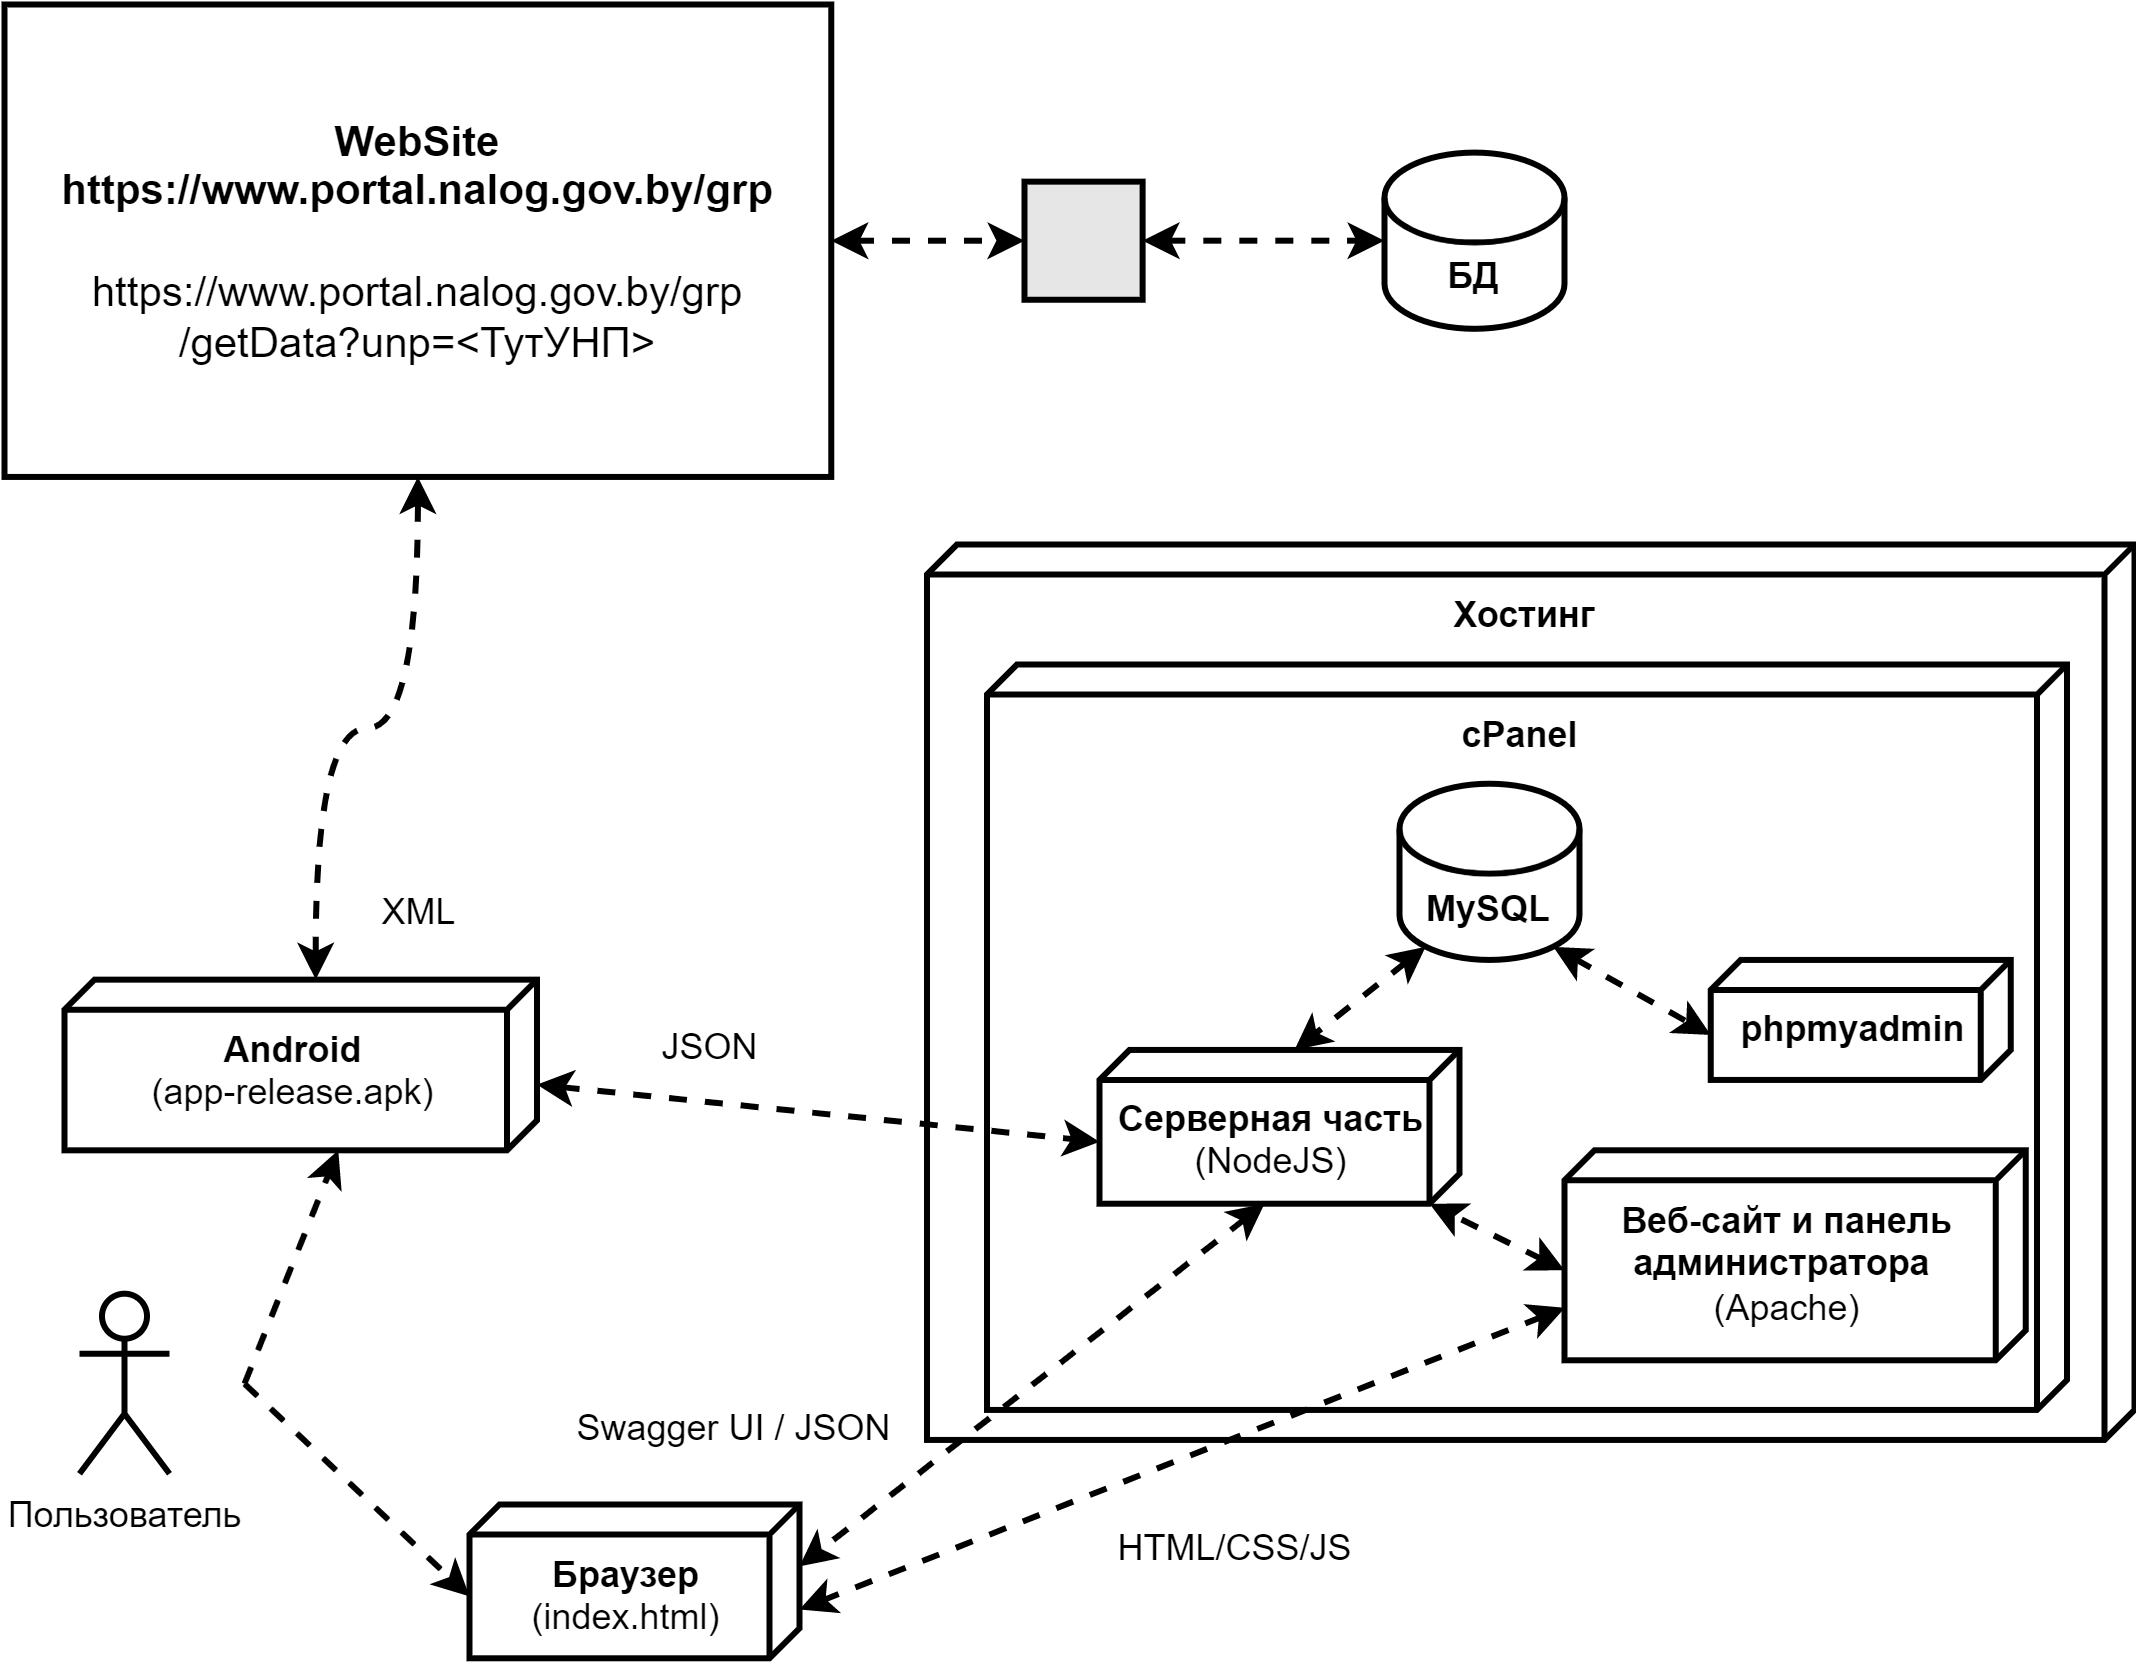
\includegraphics[width=18cm]
    {images/UML/UML_deployment_diagram_prod.png}

    \caption{Диаграмма развертывания приложения}

    \label{fig:UML_deployment_diagram_prod}
\end{figure}

\subsection*{Логическая модель}

Логическая модель - это описание данных, которые будут храниться в базе данных (БД), без учета конкретных технических решений.
Она отображает отношения между данными и определяет структуру и типы данных в БД.

Создание логической модели является важным шагом в процессе проектирования БД, так как она позволяет описать структуру БД на уровне бизнес-логики,
что обеспечивает ее лучшую понимаемость и согласованность с бизнес-потребностями.

Логическая модель описывает, какие данные будут храниться в БД, как эти данные связаны между собой и как они могут быть использованы в бизнес-процессах.
Создание логической модели позволяет избежать дублирования данных и упростить структуру БД, что уменьшает вероятность ошибок и повышает эффективность работы с данными.

В целом, создание логической модели позволяет более точно определить требования к БД,
что повышает качество и эффективность разработки приложений и уменьшает затраты на разработку и поддержку БД в долгосрочной перспективе.

Нормализация базы данных (БД) - это процесс организации данных в БД с целью устранения избыточности и повышения эффективности запросов к данным.
Нормализация позволяет разбить таблицы на более мелкие, связанные между собой таблицы,
чтобы избежать дублирования данных и обеспечить более легкое обновление и модификацию БД.

Первая нормальная форма (1НФ) - это правило, согласно которому все значения в таблице должны быть простыми, атомарными, и не должны содержать списки
или множества значений в одной ячейке.
То есть каждая ячейка таблицы должна содержать только одно значение, а не несколько значений разделенных запятыми или другим разделителем.

Вторая нормальная форма (2НФ) - это правило, согласно которому каждый столбец в таблице должен зависеть только от первичного ключа,
а не от любого другого набора столбцов. Это означает, что каждая таблица должна иметь первичный ключ и зависимые от него столбцы.

Третья нормальная форма (3НФ) - это правило, согласно которому каждый столбец, не являющийся первичным ключом,
должен зависеть только от первичного ключа,
а не от других зависимых столбцов.
Это означает, что каждый столбец должен быть функционально зависимым от первичного ключа.

Нормализация БД позволяет создавать более гибкие и эффективные БД, которые легче обновлять и модифицировать.
В результате это упрощает разработку приложений, которые работают с такими БД.

Технические названия таблиц в базе данных приведены в таблице~\ref{tab:db_table_name}.

\begin{table}[!htb]
    \centering\small

    \caption{Технические названия таблиц в БД}
    \label{tab:db_table_name}

    \begin{tabular}{|p{6cm}|p{11cm}|}
        \hline
        \multicolumn{1}{|c|}{Техническое название}
        & \multicolumn{1}{c|}{Наименование}
        \\ \hline

        DP\_CTL\_ContactTypes & справочник типов контакта \\ \hline 
        DP\_CTL\_Helpers & справочник помощников \\ \hline 
        DP\_CTL\_ItemBrands & справочник брендов \\ \hline 
        DP\_CTL\_ItemCategories & справочник категорий \\ \hline 
        DP\_CTL\_ItemCharacteristics & справочник характеристик \\ \hline 
        DP\_CTL\_Items & справочник номенклатуры \\ \hline 
        DP\_CTL\_Roles & справочник ролей \\ \hline 
        DP\_CTL\_Users & справочник пользователей \\ \hline 
        DP\_DOC\_ActivationAccount & документ об регистрации пользователя \\ \hline 
        DP\_DOC\_ApkVersions & документ об выходе новой версии Android \\ \hline 
        DP\_DOC\_Articles & документ об выходе статьи \\ \hline 
        DP\_DOC\_ChangeEmail & документ об смене электронной почты \\ \hline 
        DP\_DOC\_Orders & документ об заявке товаров \\ \hline 
        DP\_DOC\_Sessions & документ от авторизации пользователя \\ \hline 
        DP\_DOC\_UserRoles & документ об выдаче прав пользователю \\ \hline 
        DP\_LST\_ArticleAttachedLinks & список ссылок в статье \\ \hline 
        DP\_LST\_FavoriteItems & список избранных товаров \\ \hline 
        DP\_LST\_HelperContactTypes & список контактов помощника \\ \hline 
        DP\_LST\_ItemCharacteristics & список характеристик номенклатуры \\ \hline 
        DP\_LST\_ItemGalery & список картинок номенклатуры \\ \hline 
        DP\_LST\_OrderItems & список номенклатуры в заявке \\ \hline 
        DP\_migrations& миграции \\ \hline 
    \end{tabular}
\end{table}

Справочник <<Пользователи>> -
предназначен для хранения данных пользователей
(о УНП, полном наименовании юридического лица, кратком наименовании юридического лица,
адресе, телефоне приемной, фамилии, имени, отчестве,
логине, электронной почте и хэшированном пароле).
Атрибуты и типы данных указаны в таблице~\ref{tab:DP_CTL_Users}.

\begin{table}[!htb]
    \centering\small

    \caption{Атрибуты справочника <<Пользователи>>}
    \label{tab:DP_CTL_Users}
    
    \begin{tabular}{|p{5cm}|p{2.5cm}|p{9cm}|}
        \hline
        \multicolumn{1}{|c|}{Атрибут}
        & \multicolumn{1}{c|}{Тип данных}
        & \multicolumn{1}{c|}{Комментарий}
        \\ \hline

        dp\_id & varchar(36) & уникальный идентификатор \\ \hline
        dp\_login & varchar(255) & логин \\ \hline
        dp\_email & varchar(64) & электронная почта \\ \hline
        dp\_passwordHash & varchar(60) & хэш пароля \\ \hline
        dp\_unp & varchar(13) & УНП \\ \hline
        dp\_nameLegalEntity & varchar(255) & полное наименование юртдического лица \\ \hline
        dp\_shortNameLegalEntity & varchar(255) & краткое наименование юридического лица \\ \hline
        dp\_address & varchar(255) & адрес \\ \hline
        dp\_receptionPhone & varchar(13) & телефон \\ \hline
        dp\_firstName & varchar(32) & имя \\ \hline
        dp\_middleName & varchar(32) & отчество \\ \hline
        dp\_lastName & varchar(32) & фамилия \\ \hline
    \end{tabular}
\end{table}

\newpage

Документ об регистрации аккаунта -
фиксирует регистрацию пользователя. Предназначен для хранения даты регистрации,
токена активации аккаунта, идентификатора пользователя и флаге активации (истина/ложь).
Этот токен отправляется на email в ссылке. По переходу по ссылке аккаунт активируется.
Каждый час сервер проверяет таблицу на наличие записей старше 24 часа.
Если запись найдена, то это значит, что пользователь не перешел по ссылке и не активировал аккаунт.
Сервер удалит аккаунт по идентификатору пользователя.
Атрибуты и типы данных указаны в таблице~\ref{tab:DP_DOC_ActivatedAccount}.

\begin{table}[!htb]
    \centering\small

    \caption{Атрибуты документа об регистрации аккаунта}
    \label{tab:DP_DOC_ActivatedAccount}
    
    \begin{tabular}{|p{5cm}|p{2.5cm}|p{9cm}|}
        \hline
        \multicolumn{1}{|c|}{Атрибут}
        & \multicolumn{1}{c|}{Тип данных}
        & \multicolumn{1}{c|}{Комментарий}
        \\ \hline

        dp\_id & int & идентификатор \\ \hline
        dp\_date & timestamp & дата регистрации \\ \hline
        dp\_token & varchar(255) & токен, который приходит на почту \\ \hline
        dp\_userId & varchar(36) & код пользователя \\ \hline
        dp\_isActivated & tinyint & аккаунт активирован \\ \hline
    \end{tabular}
\end{table}

Документ об авторизации пользователя - фиксирует вход в аккаунт.
Предназначен для хранения IP-адреса, наименовании устройства, токена доступа, токена обновления.
Токен доступа позволяет выполнять HTTP запросы, которые разрешены авторизованому пользователю.
Токен обновления позволяет обновлять токен доступа, в случаем если он был утерян, либо просрочен.
Атрибуты и типы данных указаны в таблице~\ref{tab:DP_DOC_Sessions}.

\begin{table}[!htb]
    \centering\small

    \caption{Атрибуты документа об авторизации пользователя}
    \label{tab:DP_DOC_Sessions}

    \begin{tabular}{|p{5cm}|p{2.5cm}|p{9cm}|}
        \hline
        \multicolumn{1}{|c|}{Атрибут}
        & \multicolumn{1}{c|}{Тип данных}
        & \multicolumn{1}{c|}{Комментарий}
        \\ \hline

        dp\_id & int & идентификатор \\ \hline
        dp\_date & timestamp & дата входа в аккаунт \\ \hline
        dp\_ip & varchar(255) & IP-адрес \\ \hline
        dp\_agent & varchar(255) & устройство \\ \hline
        dp\_accessHash & varchar(60) & хэш токена доступа \\ \hline
        dp\_refreshHash & varchar(60) & хэш токена обновления \\ \hline
        dp\_userId & varchar(36) & код пользователя \\ \hline
    \end{tabular}
\end{table}

Документ об смене электронной почты - фиксирует заявку на смену старой электронной почты на новую.
Предназначена для хранения даты отправки заявки, токена для продолжения смены или отмены заявки,
старой электронной почты, новой электронной почты,
идентификатора пользователя, флага закрытия заявки (истина/ложь).
Токен отправляется на старую электронную почту в двух ссылоках.
Первая ссылка подтверждает смену электронной почты.
Вторая ссылка отменяет смену электронной почты.
Атрибуты и типы данных указаны в таблице~\ref{tab:DP_DOC_ChangeEmail}.

\begin{table}[!htb]
    \centering\small

    \caption{Атрибуты документа смены e-mail}
    \label{tab:DP_DOC_ChangeEmail}

    \begin{tabular}{|p{5cm}|p{2.5cm}|p{9cm}|}
        \hline
        \multicolumn{1}{|c|}{Атрибут}
        & \multicolumn{1}{c|}{Тип данных}
        & \multicolumn{1}{c|}{Комментарий}
        \\ \hline

        dp\_id & int & идентификатор \\ \hline
        dp\_date & timestamp & дата \\ \hline
        dp\_token & varchar(255) & токен для почты \\ \hline
        dp\_oldEmail & varchar(64) & старая электронная почта \\ \hline
        dp\_newEmail & varchar(64) & новая электронная почта \\ \hline
        dp\_userId & varchar(36) & код пользователя \\ \hline
        dp\_isClosed & tinyint & заявка закрыта, либо выполнена \\ \hline
    \end{tabular}
\end{table}

Справочник <<Роли пользователя>> - предназначена для ролей, которые можно выдать пользователю.
Атрибуты и типы данных указаны в таблице~\ref{tab:DP_CTL_Roles}.

\begin{table}[!htb]
    \centering\small

    \caption{Атрибуты каталога <<Роли пользователя>>}
    \label{tab:DP_CTL_Roles}

    \begin{tabular}{|p{5cm}|p{2.5cm}|p{9cm}|}
        \hline
        \multicolumn{1}{|c|}{Атрибут}
        & \multicolumn{1}{c|}{Тип данных}
        & \multicolumn{1}{c|}{Комментарий}
        \\ \hline

        dp\_id & int & идентификатор \\ \hline
        dp\_name & varchar(32) & наименование \\ \hline
    \end{tabular}
\end{table}

Документ о назначении роли - фиксирует выдачу роли пользователю.
Предназначена для хранения выданых ролей.
Атрибуты и типы данных указаны в таблице~\ref{tab:DP_DOC_UserRoles}.

\begin{table}[!htb]
    \centering\small

    \caption{Атрибуты документа о назначении роли}
    \label{tab:DP_DOC_UserRoles}

    \begin{tabular}{|p{5cm}|p{2.5cm}|p{9cm}|}
        \hline
        \multicolumn{1}{|c|}{Атрибут}
        & \multicolumn{1}{c|}{Тип данных}
        & \multicolumn{1}{c|}{Комментарий}
        \\ \hline

        dp\_id & int & идентификатор \\ \hline
        dp\_date & datetime & дата выдачи роли \\ \hline
        dp\_userId & varchar(36) & код пользователя \\ \hline
        dp\_roleId & int & код роли \\ \hline
    \end{tabular}
\end{table}

Справочник <<Бренды>> - предназначена для хранения производителей номенклатуры.
Атрибуты и типы данных указаны в таблице~\ref{tab:DP_CTL_ItemBrands}.

\begin{table}[!htb]
    \centering\small

    \caption{Атрибуты каталога <<Бренды>>}
    \label{tab:DP_CTL_ItemBrands}

    \begin{tabular}{|p{5cm}|p{2.5cm}|p{9cm}|}
        \hline
        \multicolumn{1}{|c|}{Атрибут}
        & \multicolumn{1}{c|}{Тип данных}
        & \multicolumn{1}{c|}{Комментарий}
        \\ \hline

        dp\_id & int & идентификатор \\ \hline
        dp\_name & varchar(255) & наименование \\ \hline
        dp\_sortingIndex & int & для сортировки \\ \hline
        dp\_urlSegment & varchar(255) & часть URL \\ \hline
        dp\_photoUrl & varchar(255) & картинка\\ \hline
        dp\_seoKeywords & varchar(255) & ключевые слова \\ \hline
        dp\_seoDescription & varchar(255) & описание \\ \hline
        dp\_isHidden & tinyint & флаг для скрытия \\ \hline
    \end{tabular}
\end{table}

Справочник <<Категории номенклатуры>> - предназначена для хранения категорий номенклатуры.
Атрибуты и типы данных указаны в таблице~\ref{tab:DP_CTL_ItemCategories}.

\begin{table}[!htb]
    \centering\small

    \caption{Атрибуты каталога <<Категории номенклатуры>>}
    \label{tab:DP_CTL_ItemCategories}

    \begin{tabular}{|p{5cm}|p{2.5cm}|p{9cm}|}
        \hline
        \multicolumn{1}{|c|}{Атрибут}
        & \multicolumn{1}{c|}{Тип данных}
        & \multicolumn{1}{c|}{Комментарий}
        \\ \hline

        dp\_id & int & идентификатор \\ \hline
        dp\_name & varchar(255) & наименование \\ \hline
        dp\_sortingIndex & int & для сортировки \\ \hline
        dp\_urlSegment & varchar(255) & часть URL\\ \hline
        dp\_photoUrl & varchar(255) & картинка\\ \hline
        \multicolumn{3}{c}{\normalsize Продолжение таблицы~\ref{tab:DP_CTL_ItemCategories} на следующей странице} \\
        % dp\_seoKeywords & varchar(255) & ключевые слова \\ \hline
        % dp\_seoDescription & varchar(255) & описание \\ \hline
        % dp\_isHidden & tinyint & флаг для скрытия \\ \hline
        % dp\_itemBrandId & int & код категории \\ \hline
    \end{tabular}
\end{table}

\begin{table}[!htb]
    \centering\small

    % \caption{Атрибуты каталога DP\_CTL\_ItemCategories}
    % \label{tab:DP_CTL_ItemCategories}

    \begin{tabular}{|p{5cm}|p{2.5cm}|p{9cm}|}
        \multicolumn{3}{c}{\normalsize Продолжение таблицы~\ref{tab:DP_CTL_ItemCategories}} \\

        \hline
        \multicolumn{1}{|c|}{Атрибут}
        & \multicolumn{1}{c|}{Тип данных}
        & \multicolumn{1}{c|}{Комментарий}
        \\ \hline

        % dp\_id & int & идентификатор \\ \hline
        % dp\_name & varchar(255) & наименование \\ \hline
        % dp\_sortingIndex & int & для сортировки \\ \hline
        % dp\_urlSegment & varchar(255) & часть URL\\ \hline
        % dp\_photoUrl & varchar(255) & картинка\\ \hline
        % \multicolumn{3}{c}{Продолжение таблицы~\ref{tab:DP_CTL_ItemCategories} на следующей странице}
        dp\_seoKeywords & varchar(255) & ключевые слова \\ \hline
        dp\_seoDescription & varchar(255) & описание \\ \hline
        dp\_isHidden & tinyint & флаг для скрытия \\ \hline
        dp\_itemBrandId & int & код категории \\ \hline
    \end{tabular}
\end{table}

Справочник <<Номенклатура>> - предназначена для хранения номенклатуры.
Атрибуты и типы данных указаны в таблице~\ref{tab:DP_CTL_Items}.
К этой номенклатуре по идентификатору привязываются списки:
характеристики номенклатуры (см. таблицу~\ref{tab:DP_LST_ItemCharacteristics});
картинки номенклатуры (см. таблицу~\ref{tab:DP_LST_ItemGalery}).

\begin{table}[!htb]
    \centering\small

    \caption{Атрибуты каталога <<Номенклатура>>}
    \label{tab:DP_CTL_Items}

    \begin{tabular}{|p{5cm}|p{2.5cm}|p{9cm}|}
        \hline
        \multicolumn{1}{|c|}{Атрибут}
        & \multicolumn{1}{c|}{Тип данных}
        & \multicolumn{1}{c|}{Комментарий}
        \\ \hline

        dp\_id & varchar(36) & идентификатор \\ \hline
        dp\_name & varchar(255) & наименование \\ \hline
        dp\_cost & float & цена \\ \hline
        dp\_model & varchar(32) & модель \\ \hline
        dp\_photoUrl & varchar(255) & картинка\\ \hline
        dp\_seoKeywords & varchar(255) & ключевые слова \\ \hline
        dp\_seoDescription & varchar(255) & описание \\ \hline
        dp\_isHidden & tinyint & флаг для скрытия \\ \hline
        dp\_itemCategoryId & int & код категории номенклатуры \\ \hline
    \end{tabular}
\end{table}


\begin{table}[!htb]
    \centering\small

    \caption{Атрибуты списка характеристик номенклатуры}
    \label{tab:DP_LST_ItemCharacteristics}

    \begin{tabular}{|p{5cm}|p{2.5cm}|p{9cm}|}
        \hline
        \multicolumn{1}{|c|}{Атрибут}
        & \multicolumn{1}{c|}{Тип данных}
        & \multicolumn{1}{c|}{Комментарий}
        \\ \hline

        dp\_id & int & идентификатор \\ \hline
        dp\_itemId & varchar(36) & код номенклатуры \\ \hline
        dp\_characteristicId & int & код характеристики \\ \hline
        dp\_value & varchar(255) & значение характеристики \\ \hline
    \end{tabular}
\end{table}

\begin{table}[!htb]
    \centering\small

    \caption{Атрибуты списка картинок номенклатуры}
    \label{tab:DP_LST_ItemGalery}

    \begin{tabular}{|p{5cm}|p{2.5cm}|p{9cm}|}
        \hline
        \multicolumn{1}{|c|}{Атрибут}
        & \multicolumn{1}{c|}{Тип данных}
        & \multicolumn{1}{c|}{Комментарий}
        \\ \hline

        dp\_id & int & идентификатор \\ \hline
        dp\_itemId & varchar(36) & код номеклатуры \\ \hline
        dp\_photoUrl & varchar(255) & картинка \\ \hline
    \end{tabular}
\end{table}

Cправочник <<Характеристики номенклатуры>> - предназначена для хранения специфических полей,
которые не указаны в справочнике <<Номенклатура>>.
Это может быть цвет, вес, высота, ширина, мощность, диаметр и др.
Атрибуты и типы данных указаны в таблице~\ref{tab:DP_CTL_Characteristics}.

\begin{table}[!htb]
    \centering\small

    \caption{Атрибуты каталога <<Характеристики номенклатуры>>}
    \label{tab:DP_CTL_Characteristics}

    \begin{tabular}{|p{5cm}|p{2.5cm}|p{9cm}|}
        \hline
        \multicolumn{1}{|c|}{Атрибут}
        & \multicolumn{1}{c|}{Тип данных}
        & \multicolumn{1}{c|}{Комментарий}
        \\ \hline

        dp\_id & int & идентификатор \\ \hline
        dp\_name & varchar(255) & наименование \\ \hline
        dp\_isHidden & tinyint & флаг скрытия элемента \\ \hline
    \end{tabular}
\end{table}

Документ о получении заявки номенклатуры - фиксирует заявку товара от авторизованого пользователя.
Атрибуты и типы данных указаны в таблице~\ref{tab:DP_DOC_OrderItems}.
Документ связан со списком - номенклатура заявки (см. таблицу~\ref{tab:DP_LST_OrderItems}).

\begin{table}[!htb]
    \centering\small

    \caption{Атрибуты документа о получении заявки номенклатуры}
    \label{tab:DP_DOC_OrderItems}

    \begin{tabular}{|p{5cm}|p{2.5cm}|p{9cm}|}
        \hline
        \multicolumn{1}{|c|}{Атрибут}
        & \multicolumn{1}{c|}{Тип данных}
        & \multicolumn{1}{c|}{Комментарий}
        \\ \hline

        dp\_id & varchar(36) & идентификатор \\ \hline
        dp\_date & timestamp & дата \\ \hline
        dp\_userId & varchar(36) & код пользователя \\ \hline
        dp\_canceledMyManager & datetime & заявка отменена менеджером \\ \hline
        dp\_canceledMyClient & datetime & заявка отменена клиентом \\ \hline
        dp\_sentedByManager & datetime & товар отправлен менеджером \\ \hline
        dp\_receiverByClient & datetime & товар получен клиентом \\ \hline
    \end{tabular}
\end{table}

\begin{table}[!htb]
    \centering\small

    \caption{Атрибуты списка DP\_LST\_OrderItems}
    \label{tab:DP_LST_OrderItems}

    \begin{tabular}{|p{5cm}|p{2.5cm}|p{9cm}|}
        \hline
        \multicolumn{1}{|c|}{Атрибут}
        & \multicolumn{1}{c|}{Тип данных}
        & \multicolumn{1}{c|}{Комментарий}
        \\ \hline

        dp\_id & varchar(36) & идентификатор \\ \hline
        dp\_orderItemsId & varchar(36) & код заказа номенклатуры \\ \hline
        dp\_itemId & varchar(36) & код номенклатуры \\ \hline
        dp\_count & int & количество \\ \hline
        dp\_cost & float & цена \\ \hline
    \end{tabular}
\end{table}

Документ о смене статуса заказа - заполняется менеджером и информирует
пользователя и продвижении заявки в его мобильном приложении.
Атрибуты и типы данных указаны в таблице~\ref{tab:DP_DOC_OrderStatuses}.

\begin{table}[!htb]
    \centering\small

    \caption{Атрибуты документа о смене статуса заказа}
    \label{tab:DP_DOC_OrderStatuses}

    \begin{tabular}{|p{5cm}|p{2.5cm}|p{9cm}|}
        \hline
        \multicolumn{1}{|c|}{Атрибут}
        & \multicolumn{1}{c|}{Тип данных}
        & \multicolumn{1}{c|}{Комментарий}
        \\ \hline

        dp\_id & varchar(36) & идентификатор \\ \hline
        dp\_date & timestamp & дата \\ \hline
        dp\_status & varchar(255) & статус \\ \hline
        dp\_orderItemsId & varchar(36) & код заказа номенклатуры \\ \hline
    \end{tabular}
\end{table}

Справочник <<Помощники>> - предназначен для хранения данных организации, которые будут доступны обществености.
Атрибуты и типы данных указаны в таблице~\ref{tab:DP_CTL_Helpers}.
Список этого справочника будет показан на странице контактов,
чтобы клиент мог обратится по удобному ему виду связи:
телефон; e-mail, Viber, Telegram, WhatsApp, Skype.
Этот справочник имеет список - список контактов (см. таблицу~\ref{tab:DP_LST_HelperContacts}).

\begin{table}[!htb]
    \centering\small

    \caption{Атрибуты каталога <<Помощники>>}
    \label{tab:DP_CTL_Helpers}

    \begin{tabular}{|p{5cm}|p{2.5cm}|p{9cm}|}
        \hline
        \multicolumn{1}{|c|}{Атрибут}
        & \multicolumn{1}{c|}{Тип данных}
        & \multicolumn{1}{c|}{Комментарий}
        \\ \hline

        dp\_id & varchar(36) & идентификатор \\ \hline
        dp\_name & varchar(255) & наименование \\ \hline
        dp\_text & varchar(255) & описание \\ \hline
        dp\_sortingIndex & int & индекс для сортировки \\ \hline
        dp\_isHidden & tinyint & флаг для скрытия элемента \\ \hline
    \end{tabular}
\end{table}

\begin{table}[!htb]
    \centering\small

    \caption{Атрибуты списка контактов помощников}
    \label{tab:DP_LST_HelperContacts}

    \begin{tabular}{|p{5cm}|p{2.5cm}|p{9cm}|}
        \hline
        \multicolumn{1}{|c|}{Атрибут}
        & \multicolumn{1}{c|}{Тип данных}
        & \multicolumn{1}{c|}{Комментарий}
        \\ \hline

        dp\_id & varchar(36) & идентификатор \\ \hline
        dp\_helperId & varchar(36) & код помощника \\ \hline
        dp\_contactTypeId & int & код типа контакта \\ \hline
        dp\_value & varchar(255) & значение контакта \\ \hline
    \end{tabular}
\end{table}

Cправочник <<Типы контакта>> - предназначена для хранения специфических полей, которых нет в справочнике <<Помощники>>.
Атрибуты и типы данных указаны в таблице~\ref{tab:DP_CTL_ContactTypes}.

\begin{table}[!htb]
    \centering\small

    \caption{Атрибуты каталога <<Типы контакта>>}
    \label{tab:DP_CTL_ContactTypes}

    \begin{tabular}{|p{5cm}|p{2.5cm}|p{9cm}|}
        \hline
        \multicolumn{1}{|c|}{Атрибут}
        & \multicolumn{1}{c|}{Тип данных}
        & \multicolumn{1}{c|}{Комментарий}
        \\ \hline

        dp\_id & int & идентификатор \\ \hline
        dp\_name & varchar(255) & наименование \\ \hline
        dp\_isHidden & tinyint & флаг скрытия элемента \\ \hline
    \end{tabular}
\end{table}

Документ о создании статьи (аналог новостей, аналог блога) - фиксирует написание статьи по дате.
Атрибуты и типы данных указаны в таблице~\ref{tab:DP_DOC_Articles}.
Документ может содержать список - список прикрепленых ссылок (см. таблицу~\ref{tab:DP_LST_ArticleAttachedLinks}).
Ссылка может указывать на PDF файлы, которые может качать пользователь.

\begin{table}[!htb]
    \centering\small

    \caption{Атрибуты документа о создании статьи}
    \label{tab:DP_DOC_Articles}

    \begin{tabular}{|p{5cm}|p{2.5cm}|p{9cm}|}
        \hline
        \multicolumn{1}{|c|}{Атрибут}
        & \multicolumn{1}{c|}{Тип данных}
        & \multicolumn{1}{c|}{Комментарий}
        \\ \hline

        dp\_id & varchar(36) & идентификатор \\ \hline
        dp\_name & varchar(255) & наименование \\ \hline
        dp\_date & timestamp & дата \\ \hline
        dp\_photoUrl & varchar(255) & ссылка на картинку \\ \hline
        dp\_text & varchar(4096) & текст статьи \\ \hline
        dp\_urlSegment & varchar(255) & часть URL \\ \hline
        dp\_sortingIndex & int & индекс для сортировки \\ \hline
        dp\_seoKeywords & varchar(255) & ключевые слова \\ \hline
        dp\_seoDescription & varchar(255) & описание \\ \hline
        dp\_isHidden & tinyint & флаг скрытия \\ \hline
    \end{tabular}
\end{table}

\begin{table}[!htb]
    \centering\small

    \caption{Атрибуты списка ссылок прикрепленых статье}
    \label{tab:DP_LST_ArticleAttachedLinks}

    \begin{tabular}{|p{5cm}|p{2.5cm}|p{9cm}|}
        \hline
        \multicolumn{1}{|c|}{Атрибут}
        & \multicolumn{1}{c|}{Тип данных}
        & \multicolumn{1}{c|}{Комментарий}
        \\ \hline

        dp\_id & varchar(36) & идентификатор \\ \hline
        dp\_articleId & varchar(36) & код статьи \\ \hline
        dp\_name & varchar(255) & наименование ссылки \\ \hline
        dp\_url & varchar(255) & ссылка на файл \\ \hline
    \end{tabular}
\end{table}

При добавлении номенклатуры в избранные - номенклатуры фиксируется в списке изабранных.
Атрибуты и типы данных указаны в таблице~\ref{tab:DP_LST_FavoriteItems}.

\begin{table}[!htb]
    \centering\small

    \caption{Атрибуты списка избранных}
    \label{tab:DP_LST_FavoriteItems}

    \begin{tabular}{|p{5cm}|p{2.5cm}|p{9cm}|}
        \hline
        \multicolumn{1}{|c|}{Атрибут}
        & \multicolumn{1}{c|}{Тип данных}
        & \multicolumn{1}{c|}{Комментарий}
        \\ \hline

        dp\_id & varchar(36) & идентификатор \\ \hline
        dp\_itemId & varchar(36) & код номенклатуры \\ \hline
        dp\_userId & int & код пользователя \\ \hline
    \end{tabular}
\end{table}

Логическая модель системы, отражающая связи и структуру данных,
используемых в системе,
представлена на рисунке~\ref{fig:db_logic_model}.

% Рисунок~\ref{fig:db_logic_model} представляет логическую модель системы,
% описывающую связи и структуру данных, используемых в системе.

% Логическая модель изображена на рис.~\ref{fig:db_logic_model}.

\begin{figure}[!p]
    \centering

    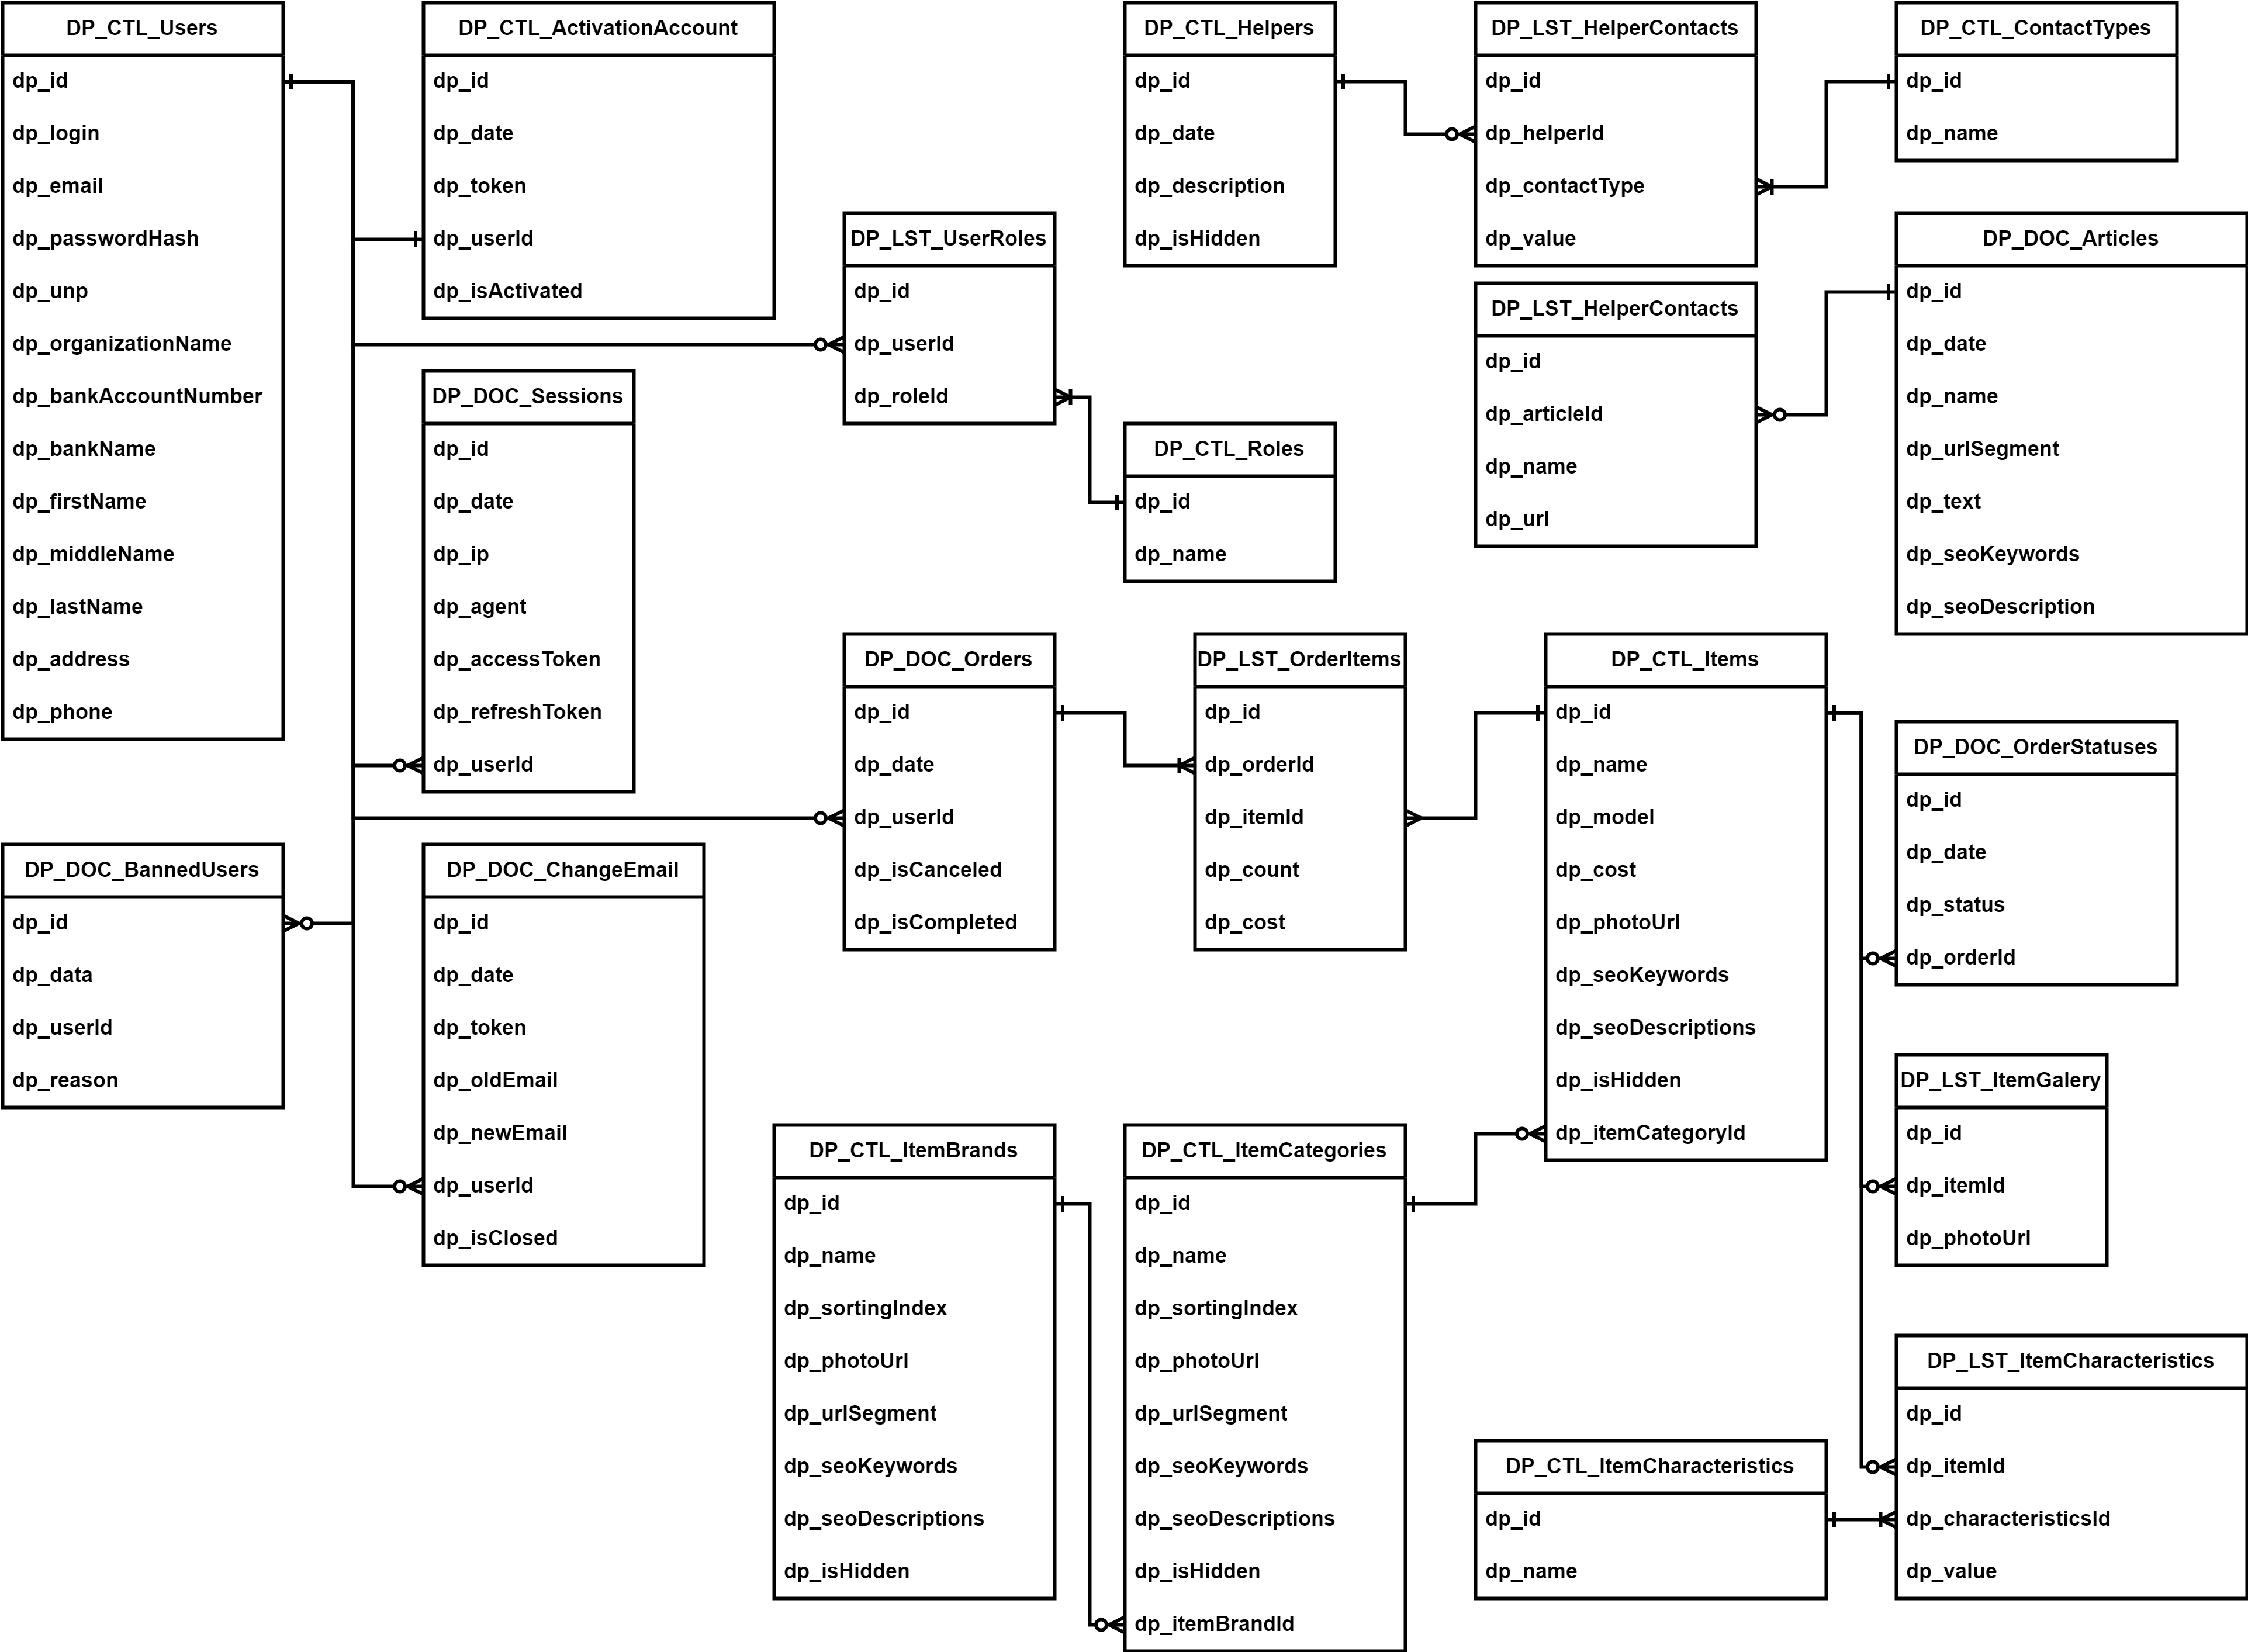
\includegraphics[angle=90, width=18cm]
    {images/db/db.png}

    \caption{Логическая модель}

    \label{fig:db_logic_model}
\end{figure}

\subsection{Физическая модель}

При работе с базами данных в NestJS, может понадобиться изменение её структуры, например, добавление новых таблицы или изменение существующих.
Для этого в NestJS используются миграции.

Миграции - это специальные файлы, которые содержат инструкции для изменения структуры базы данных.
Они позволяют изменять схему базы данных без необходимости вручную изменять ее структуру.

В NestJS миграции генерируются с помощью инструмента командной строки TypeORM.
Для генерации новой миграции необходимо использовать команду <<typeorm migration:generate>>.
В этой команде указаваем имя миграции.

Когда миграция готова, можно применить её к базе данных, используя команду <<typeorm migration:run>>.
Эта команда выполнит все новые миграции и обновит структуру базы данных в соответствии изменениями.

Таким образом, генерация миграций в NestJS с помощью TypeORM позволяет управлять изменениями в базе данных и обеспечивает более безопасную работу с данными.

TypeORM также предоставляет команду <<migration:revert>>, которая позволяет отменять миграции и откатывать изменения, сделанные в базе данных.

Команда <<migration:revert>> используется для отмены последней примененной миграции.
Это означает, что если уже применили миграцию к базе данных с помощью команды <<migration:run>>,
то команда <<migration:revert>> откатит последнее изменение в базе данных, которое было сделано в этой миграции.


\newpage
\section{РЕАЛИЗАЦИЯ И ТЕСТИРОВАНИЕ СИСТЕМЫ}
% \textbf{Swagger UI} - это инструмент для визуализации и тестирования RESTful API,
который позволяет легко и удобно отображать документацию API в интерактивном формате.
Swagger UI позволяет пользователям легко узнать, как использовать API, просматривать доступные методы и параметры, а также тестировать их напрямую из интерфейса.

NestJS предоставляет мощный интегрированный инструмент для создания и документирования API - Swagger Module.
Этот модуль автоматически генерирует документацию API на основе встроенных декораторов и аннотаций,
что делает процесс создания документации проще и быстрее.
Кроме того, Swagger Module позволяет легко интегрировать Swagger UI в приложение,
чтобы пользователи могли удобно просматривать и тестировать API.

При использовании NestJS и Swagger Module, можено значительно сократить время и усилия,
затрачиваемые на создание и документирование API.
NestJS обеспечивает простоту и гибкость при создании API, а Swagger Module делает процесс документирования быстрым и удобным.
Кроме того, Swagger UI предоставляет простой и понятный интерфейс для тестирования API,
что делает процесс отладки более эффективным. Все это делает NestJS лучшим выбором для создания и документирования API,
особенно если хотим сэкономить время и усилия при разработке.

\textbf{Эндпоинт} (англ. endpoint) - это конечная точка (адрес) веб-сервера, доступная для запросов от клиентского приложения.
В контексте веб-разработки эндпоинт обычно является частью RESTful API (Representational State Transfer API)
и представляет собой конечную точку, к которой можно отправить запросы для выполнения определенного действия или получения определенной информации.

Например, если мы хотим получить информацию о товаре с определенным идентификатором,
мы можем отправить запрос на эндпоинт веб-сервера, который обрабатывает такие запросы и возвращает запрашиваемую информацию в определенном формате,
например, JSON или XML.

Эндпоинт может обрабатывать различные типы запросов, такие как GET, POST, PATCH, PUT или DELETE,
в зависимости от того, какие действия должны быть выполнены с данными на сервере.
Кроме того, эндпоинт может быть защищен авторизацией, чтобы предотвратить несанкционированный доступ к конфиденциальным данным или функциональности.

\textbf{Эндпоинт <<users>>} связан с управлением учётными записями пользователей.
Благодаря данному эндпоинту, пользователи имеют возможность выполнять следующие операции:
регистрацию новой учётной записи,
активацию аккаунта,
запрос на смену электронной почты,
подтверждение смены адреса электронной почты,
отмену запроса на смену адреса электронной почты,
восстановление забытого пароля,
а также изменение пароля текущей учётной записи.

Эндпоинт <<users>> представлен на рис.~\ref{fig:swagger_users}.

\begin{figure}[!p]
    \centering

    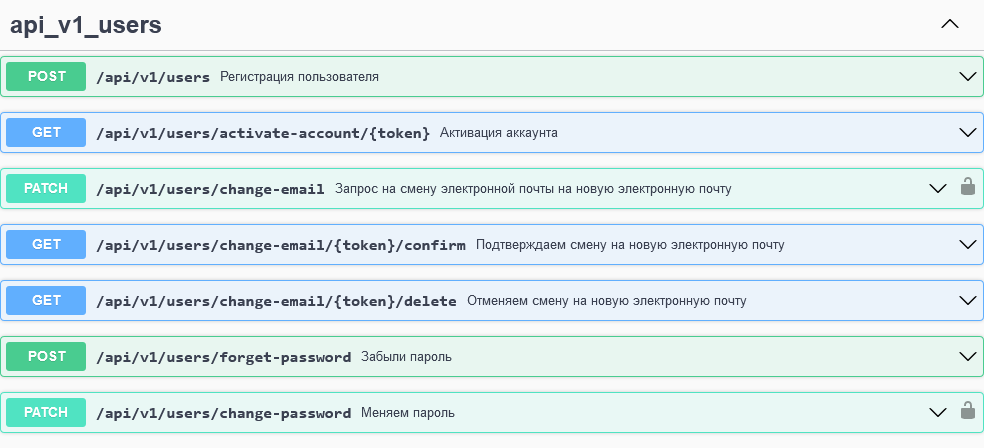
\includegraphics[width=12cm]
    {images/swagger/users.png}

    \caption{Эндпоинт <<users>>}

    \label{fig:swagger_users}
\end{figure}

\textbf{Эндпоинт <<sessions>>} в приложении играет важную роль,
предоставляя возможность пользователям войти в свой аккаунт и получить доступ к различным функциям.
С помощью этого эндпоинта можно получить доступ к списку активных сессий,
обновить существующую сессию для получения нового токенов доступа.
Также эндпоинт <<sessions>> позволяет закрыть текущую сессию или все активные сессии,
что обеспечивает безопасность аккаунта пользователя.
В целом, этот эндпоинт является важным инструментом для управления сессиями пользователей и обеспечения безопасности данных в приложении.

Эндпоинт <<sessions>> представлен на рис.~\ref{fig:swagger_sessions}.

\begin{figure}[!p]
    \centering

    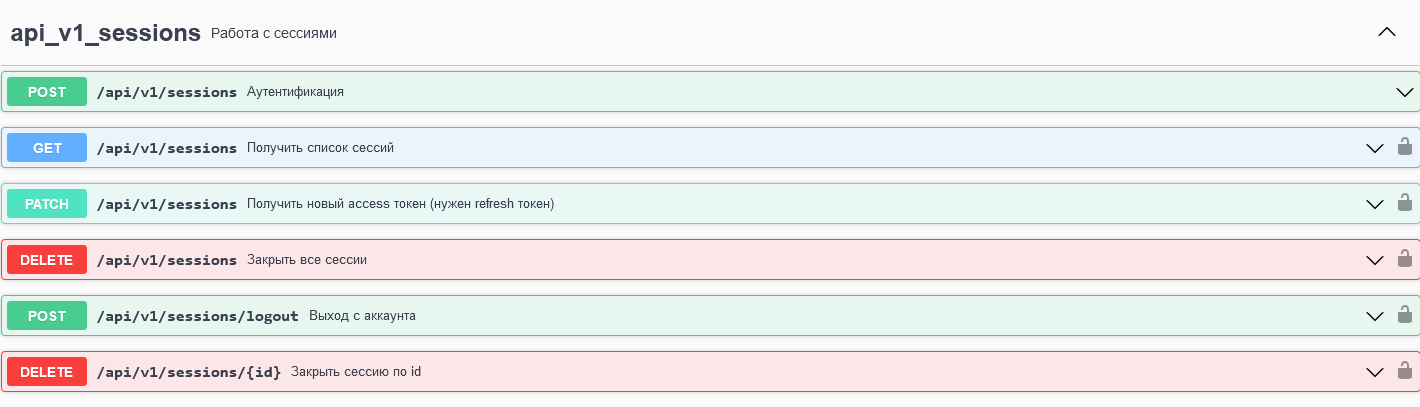
\includegraphics[width=12cm]
    {images/swagger/sessions.png}

    \caption{Эндпоинт <<sessions>>}

    \label{fig:swagger_sessions}
\end{figure}

\textbf{Эндпоинт item-brands} предназначен для осуществления операций CRUD (Create, Read, Update, Delete) с производителями номенклатуры.
Здесь вы можете создавать новых производителей, просматривать информацию о них, обновлять данные и удалять производителей, если это необходимо

Эндпоинт <<item-brands>> представлен на рис.~\ref{fig:swagger_item_brands}.

\begin{figure}[!p]
    \centering

    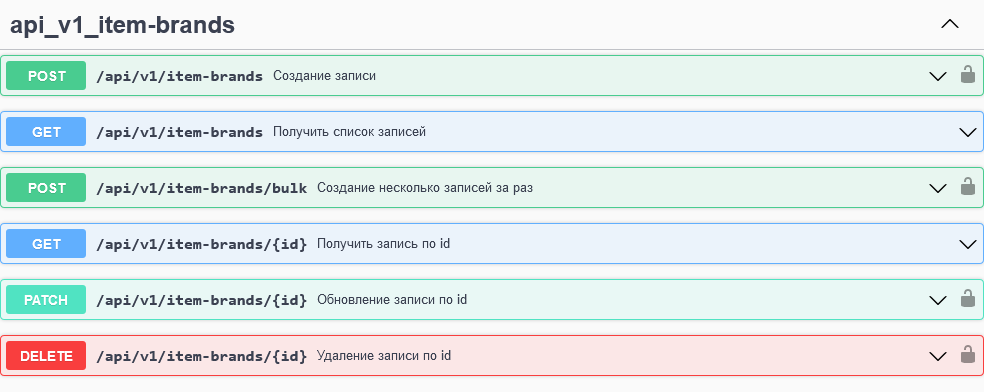
\includegraphics[width=12cm]
    {images/swagger/item-brands.png}

    \caption{Эндпоинт <<item-brands>>}

    \label{fig:swagger_item_brands}
\end{figure}

\textbf{Эндпоинт item-categories} предназначен для управления категориями номенклатуры,
включающего в себя операции CRUD (Create, Read, Update, Delete).
Здесь вы сможете создавать, просматривать, обновлять и удалять категории, а также получать информацию о них.

Эндпоинт <<item-brands>> представлен на рис.~\ref{fig:swagger_item_categories}.

\begin{figure}[!p]
    \centering

    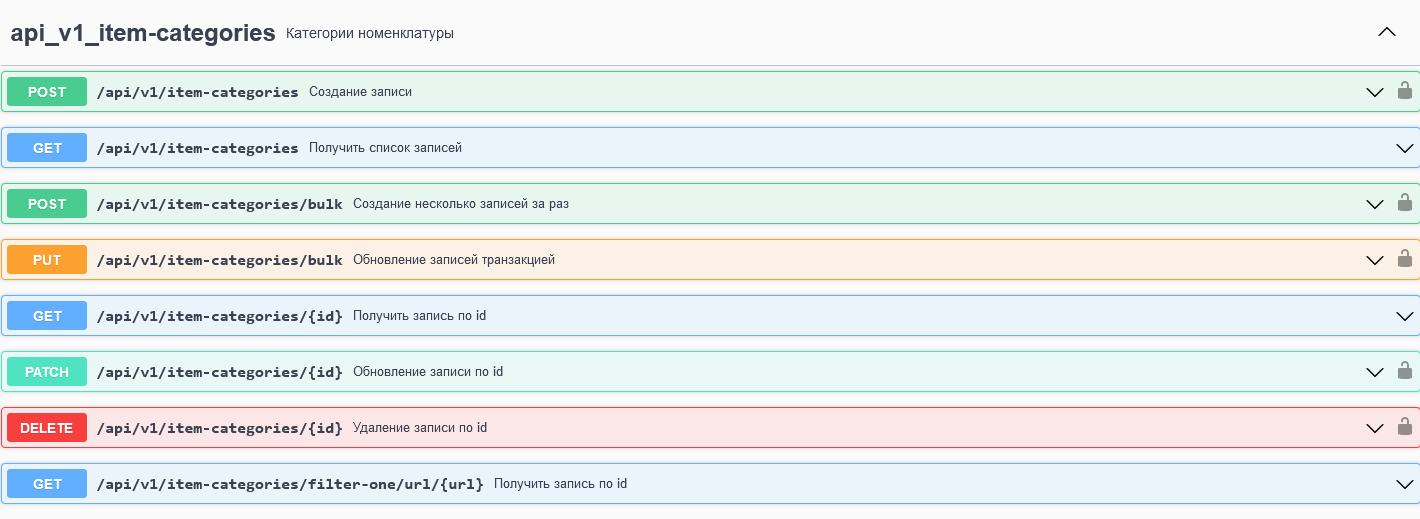
\includegraphics[width=12cm]
    {images/swagger/item-categories.png}

    \caption{Эндпоинт <<item-categories>>}

    \label{fig:swagger_item_categories}
\end{figure}

\textbf{Эндпоинт <<item-characteristics>>} обеспечивает набор CRUD-операций для типов характеристик номенклатуры.

Эндпоинт <<item-characteristics>> представлен на рис.~\ref{fig:swagger_item_characteristics}.

\begin{figure}[!p]
    \centering

    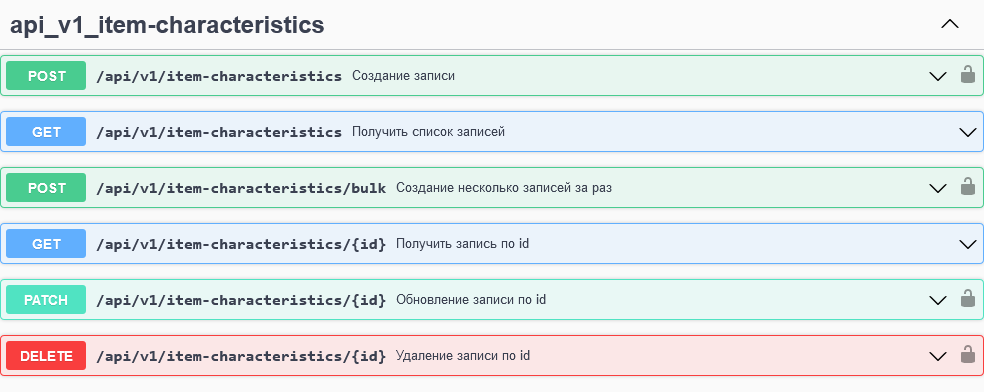
\includegraphics[width=16cm]
    {images/swagger/item-characteristics.png}

    \caption{Эндпоинт <<item-characteristics>>}

    \label{fig:swagger_item_characteristics}
\end{figure}

\textbf{Эндпоинт <<items>>} представляет набор операций CRUD для управления номенклатурой.
Кроме того, он позволяет добавлять и редактировать табличные части, включая список характеристик номенклатуры и ссылок на картинки.
Это дает возможность удобно и эффективно управлять всей информацией, связанной с конкретной номенклатурой в едином месте.

Эндпоинт <<items>> представлен на рис.~\ref{fig:swagger_items}.

\begin{figure}[!p]
    \centering

    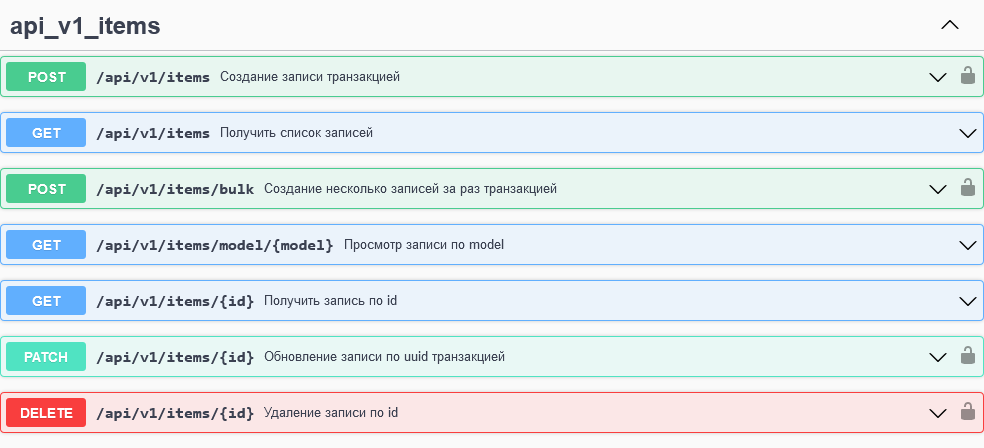
\includegraphics[width=16cm]
    {images/swagger/items.png}

    \caption{Эндпоинт <<items>>}

    \label{fig:swagger_items}
\end{figure}

\textbf{Эндпоинт <<articles>>} предоставляет возможность выполнения операций CRUD (Create, Read, Update, Delete) для управления статьями в приложении,
такими как новости или блог.
С помощью этого эндпоинта можно создавать, читать, обновлять и удалять статьи,
а также получать список всех статей или выборочно по фильтру.

Эндпоинт <<articles>> представлен на рис.~\ref{fig:swagger_articles}.

\begin{figure}[!p]
    \centering

    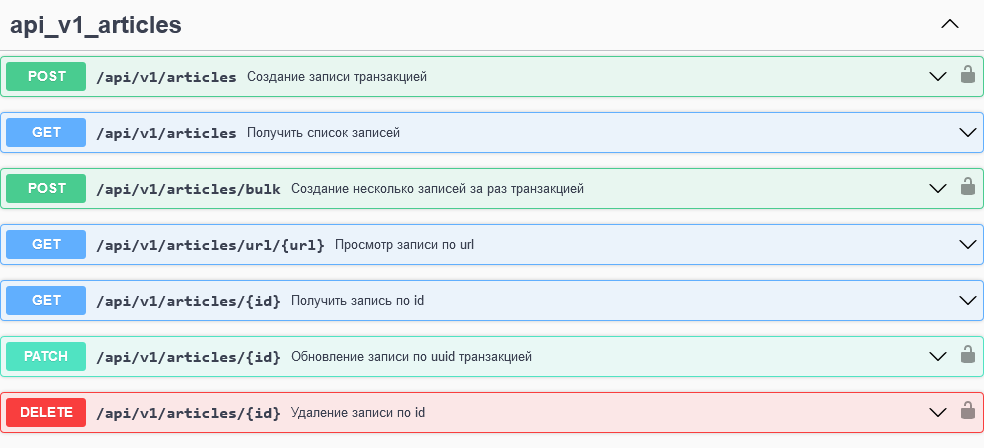
\includegraphics[width=16cm]
    {images/swagger/articles.png}

    \caption{Эндпоинт <<articles>>}

    \label{fig:swagger_articles}
\end{figure}

\textbf{Эндпоинт <<contact-types>>} представляет собой CRUD-интерфейс для управления типами контактов,
таких как email, phone, viber, whatsapp, telegram, skype.
Они являются ключевыми элементами для связи многих к одному и многих ко многим.

Эндпоинт <<contact-types>> представлен на рис.~\ref{fig:swagger_contact_types}.

\begin{figure}[!p]
    \centering

    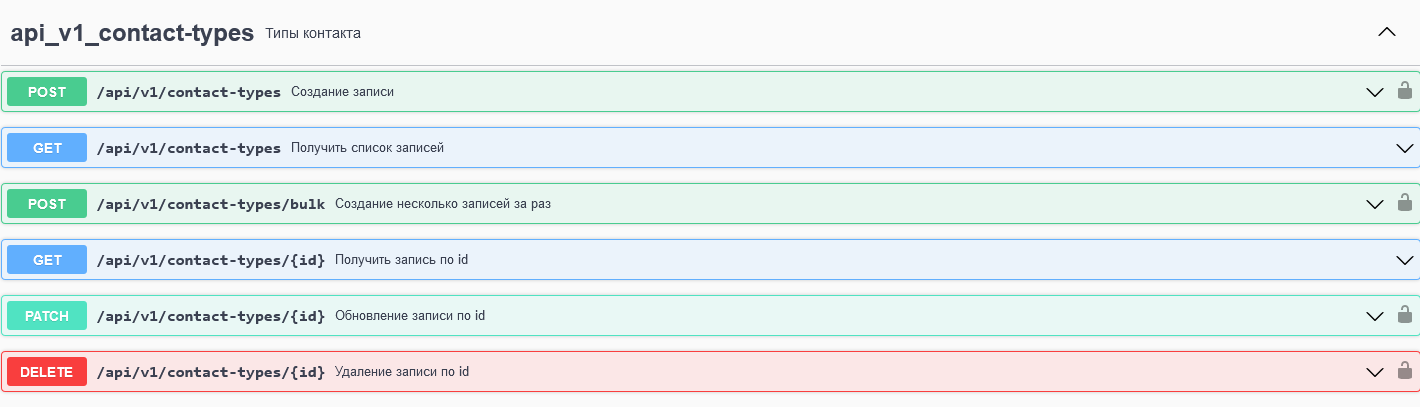
\includegraphics[width=16cm]
    {images/swagger/contact-types.png}

    \caption{Эндпоинт <<contact-types>>}

    \label{fig:swagger_contact_types}
\end{figure}

\textbf{Эндпоинт <<helpers>>} представляет полноценный CRUD-интерфейс для создания и управления контактами,
которые помогают клиентам быстро и легко связаться с компанией.
Этот эндпоинт также включает в себя удобную табличную часть,
которая позволяет добавлять и редактировать различные типы контактов,
такие как email, phone, viber, whatsapp, telegram, skype, для удобства клиентов.

Эндпоинт <<helpers>> представлен на рис.~\ref{fig:swagger_helpers}.

\begin{figure}[!p]
    \centering

    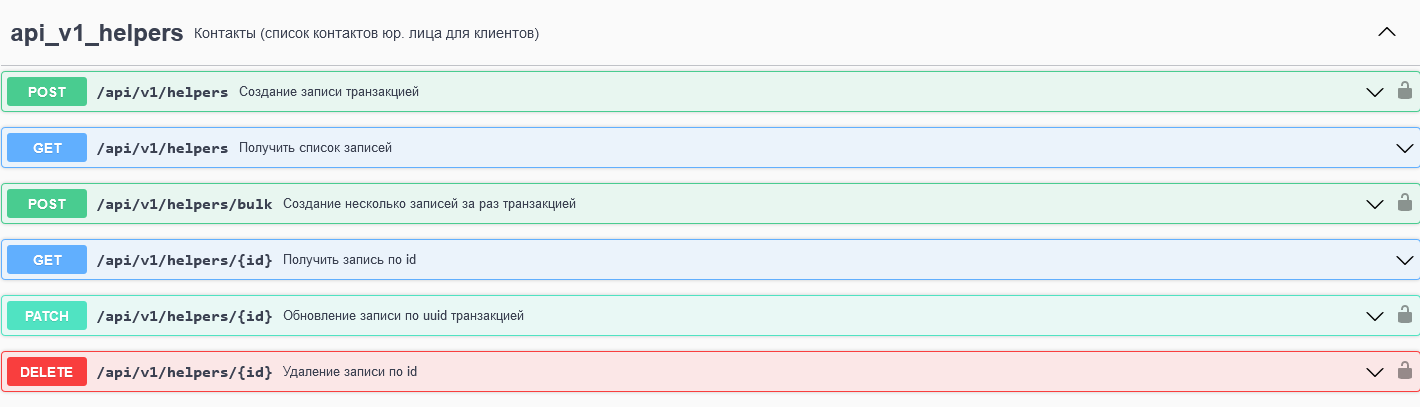
\includegraphics[width=16cm]
    {images/swagger/helpers.png}

    \caption{Эндпоинт <<helpers>>}

    \label{fig:swagger_helpers}
\end{figure}

\textbf{Эндпоинт <<orders>>} представляет собой важный механизм оформления заказов.
Он позволяет пользователям отправлять заявки на приобретение товаров,
которые затем записываются в базу данных.
Кроме того, эндпоинт позволяет отменять заказы и помечать их как закрытые модераторами, когда номенклатура уже доставлена. 

Эндпоинт <<orders>> представлен на рис.~\ref{fig:swagger_orders}.

\textbf{Экраны с номенклатурой} на Android изображены на рис.~\ref{fig:android_items}.
\textbf{Экраны со статьями} на Android изображены на рис.~\ref{fig:android_articles}.
\textbf{Экраны с корзиной и указанием количества} изображены на рис.~\ref{fig:android_basket}.
\textbf{Экраны с входом в аккаунт, восстановлением пароля и проверки обновления} изображены на рис.~\ref{fig:android_login}.
\textbf{Экраны с регистрацией юридического лица} изображены на рис.~\ref{fig:android_registration}.

\begin{figure}[!p]
    \centering

    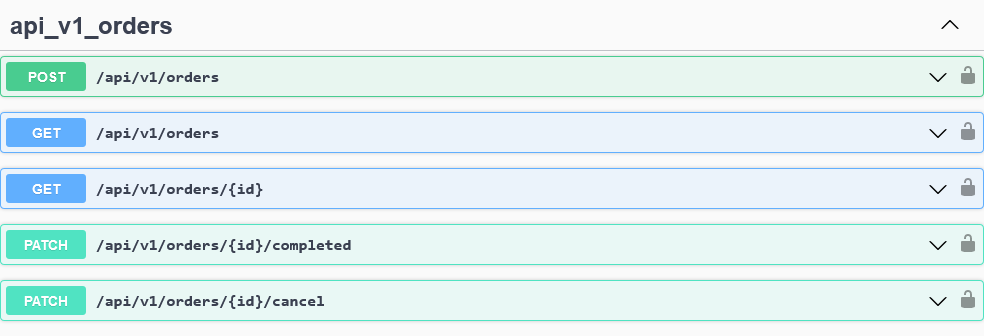
\includegraphics[width=16cm]
    {images/swagger/orders.png}

    \caption{Эндпоинт <<orders>>}

    \label{fig:swagger_orders}
\end{figure}

\begin{figure}[!p]\centering
    \begin{minipage}{0.24\textwidth}
        \centering

        \includegraphics[height=7cm]
        {images/android/item-brands.jpg}
    \end{minipage}
    \begin{minipage}{0.24\textwidth}
        \centering

        \includegraphics[height=7cm]
        {images/android/item-categories.jpg}
    \end{minipage}
    \begin{minipage}{0.24\textwidth}
        \centering

        \includegraphics[height=7cm]
        {images/android/items.jpg}
    \end{minipage}
    \begin{minipage}{0.24\textwidth}
        \centering

        \includegraphics[height=7cm]
        {images/android/item.jpg}
    \end{minipage}

    \caption{Производители, категории, товары и сам товар}
    \label{fig:android_items}
\end{figure}

\begin{figure}[!p]\centering
    \begin{minipage}{0.19\textwidth}
        \centering

        \includegraphics[width=.99\linewidth]
        {images/android/articles.jpg}
    \end{minipage}
    \begin{minipage}{0.19\textwidth}
        \centering

        \includegraphics[width=.99\linewidth]
        {images/android/article-prices.jpg}
    \end{minipage}
    \begin{minipage}{0.19\textwidth}
        \centering

        \includegraphics[width=.99\linewidth]
        {images/android/article-catalogs.jpg}
    \end{minipage}
    \begin{minipage}{0.19\textwidth}
        \centering

        \includegraphics[width=.99\linewidth]
        {images/android/article-certificates.jpg}
    \end{minipage}
    \begin{minipage}{0.19\textwidth}
        \centering

        \includegraphics[width=.99\linewidth]
        {images/android/article-contacts.jpg}
    \end{minipage}

    \caption{Прайсы, каталоги, сертификаты, контакты}
    \label{fig:android_articles}
\end{figure}

\begin{figure}[!p]\centering
    \begin{minipage}{0.49\textwidth}
        \centering

        \includegraphics[height=6cm]
        {images/android/basket.jpg}
    \end{minipage}
    \begin{minipage}{0.49\textwidth}
        \centering

        \includegraphics[height=6cm]
        {images/android/basket-change.jpg}
    \end{minipage}

    \caption{Корзина}
    \label{fig:android_basket}
\end{figure}

\begin{figure}[!p]\centering
    \begin{minipage}{0.24\textwidth}
        \centering

        \includegraphics[height=9cm]
        {images/android/account.jpg}
    \end{minipage}
    \begin{minipage}{0.24\textwidth}
        \centering

        \includegraphics[height=9cm]
        {images/android/account-login.jpg}
    \end{minipage}
    \begin{minipage}{0.24\textwidth}
        \centering

        \includegraphics[height=9cm]
        {images/android/account-forget-password.jpg}
    \end{minipage}
    \begin{minipage}{0.24\textwidth}
        \centering

        \includegraphics[height=9cm]
        {images/android/account-versions.jpg}
    \end{minipage}

    \caption{Вход в аккаунт, восстановление пароля, проверка новой версии}
    \label{fig:android_login}
\end{figure}

\begin{figure}[!p]\centering
    \begin{minipage}{0.24\textwidth}
        \centering

        \includegraphics[height=10cm]
        {images/android/account-registration-step1.jpg}
    \end{minipage}
    \begin{minipage}{0.24\textwidth}
        \centering

        \includegraphics[height=10cm]
        {images/android/account-registration-step2.jpg}
    \end{minipage}
    \begin{minipage}{0.24\textwidth}
        \centering

        \includegraphics[height=10cm]
        {images/android/account-registration-step3.jpg}
    \end{minipage}
    \begin{minipage}{0.24\textwidth}
        \centering

        \includegraphics[height=10cm]
        {images/android/account-registration-step4.jpg}
    \end{minipage}

    \caption{Регистрация юридического лица}
    \label{fig:android_registration}
\end{figure}


\newpage
\section{РАСЧЁТ ЭКОНОМИЧЕСКИХ ПОКАЗАТЕЛЕЙ}
Задачей данного дипломного проекта является
разработка серверной части на NestJS на языке программирования TypeScript,
разработка мобильного приложения на React Native на языке программирования TypeScript
и разработка веб-приложения с панелью администратора и менеджера на Create-React-App на языке программирования TypeScript.

Последовательность расчетов:

\begin{enumerate}
    \item[-] расчёт объёма функций программного модуля;
    \item[-] расчёт полной себестоимости прошраммного продукта.
\end{enumerate}

\subsection{Расчёт объема функций}

Общий объем ПО определяется по формлуле (\ref{equ:v0}) исходя из объёма функций, реализуемой программой.

\begin{equation}
    \label{equ:v0}
    \text{V}_0 = \sum^\text{n}_{\text{i}=0} \text{V}_\text{i} \text{, где}
\end{equation}

\begin{enumerate}
    \item[-] $\text{V}_0$ - общий объем части ПО; 
    \item[-] $\text{V}_\text{i}$ - объём функций части ПО;  
    \item[-] $\text{n}$ - общее число функций.
\end{enumerate}

В том случае, когда на стадии технико-экономического обоснования проекта невозможно рассчитать точный объем функций,
то на данный объём может быть получен на основании прогнозируемой оценки имеющихся фактических данных по анологичным проектам, выполненным ранее,
или применением нормативов по каталогу функций.

По каталогу фукнкий на соновании функций разрабатываемого ПО определяется общий объём ПО.
Также на основе зависимостей от организационных и технологических условий,
был скорректирован объём на основе экспертных оценок.

Уточнённый объём ПО ($\text{V}_\text{y}$) определяется по формуле (\ref{equ:vi}).

\begin{equation}
    \label{equ:vi}
    \text{V}_\text{y} = \sum^\text{n}_{\text{i}=0} \text{V}_\text{yi}
\end{equation}

\begin{enumerate}
    \item[] $\text{V}_\text{yi}$ - уточнённый объем отдельной функции в строках исходного кода.
\end{enumerate}

Перечень и объем функций ПО приведём в таблице~\ref{tab:vPO}.

\begin{table}[h!]
    \centering\small

    \caption{Перечень и объём функций программного обеспечения}
    \label{tab:vPO}

    \begin{tabular}{|p{1cm}|p{8.5cm}|p{3cm}|p{3cm}|} 
        \hline
        \multicolumn{1}{|c|}{№}
        & \multicolumn{1}{c|}{Наименование}
        & \multicolumn{2}{c|}{Объем функции строк} \\

        \multicolumn{1}{|c|}{функции}
        & \multicolumn{1}{c|}{(содержание)}
        & \multicolumn{2}{c|}{исходного кода} \\ \hline

        \multicolumn{1}{|c|}{x}
        & \multicolumn{1}{c|}{x}
        & \multicolumn{1}{c|}{По каталогу $\text{V}_\text{i}$}
        & \multicolumn{1}{c|}{Уточнённый $\text{V}_\text{yi}$} \\ \hline

        \multicolumn{1}{|c|}{101} & Организация ввода информации                            & \multicolumn{1}{r|}{130 } & \multicolumn{1}{r|}{75  } \\ \hline
        \multicolumn{1}{|c|}{102} & Контроль, предварительная обработка и ввод информации   & \multicolumn{1}{r|}{250 } & \multicolumn{1}{r|}{221 } \\ \hline
        \multicolumn{1}{|c|}{207} & Организация поиска и поиск в базе данных                & \multicolumn{1}{r|}{4720} & \multicolumn{1}{r|}{102 } \\ \hline
        \multicolumn{1}{|c|}{209} & Загрузки базы данных                                    & \multicolumn{1}{r|}{2360} & \multicolumn{1}{r|}{100 } \\ \hline
        \multicolumn{1}{|c|}{305} & Формирование файла                                      & \multicolumn{1}{r|}{2130} & \multicolumn{1}{r|}{680 } \\ \hline
        \multicolumn{1}{|c|}{707} & Графический вывод результатов                           & \multicolumn{1}{r|}{420 } & \multicolumn{1}{r|}{214 } \\ \hline
        \multicolumn{1}{|c|}{801} & Простой поиск контента портала                          & \multicolumn{1}{r|}{570 } & \multicolumn{1}{r|}{163 } \\ \hline
        \multicolumn{1}{|c|}{805} & Создание карты сайта                                    & \multicolumn{1}{r|}{76  } & \multicolumn{1}{r|}{8   } \\ \hline
        \multicolumn{1}{|c|}{806} & Сбор статистики и посетителей сайта                     & \multicolumn{1}{r|}{95  } & \multicolumn{1}{r|}{38  } \\ \hline

        \multicolumn{1}{|c|}{-}   & Всего                                                   & \multicolumn{1}{r|}{10751}& \multicolumn{1}{r|}{1601} \\ \hline
    \end{tabular}
\end{table}

С учётом информации, указанной в таблице~\ref{tab:vPO}, уточнённый объем ПО составил 1601 строка кода
вместо предпологаемого количества 10751.

Количество строк кода на текущий момент, принимая во внимание, что проекты разрабатывались с нуля \cite{LinuxCloc}:
\begin{enumerate}
    \item[-] серверная часть (backend) - 16340 строк кода;
    \item[-] мобильное приложение (frontend) - 5748 строк кода;
    \item[-] веб-приложение с панелью администратора (frontend) - 4529 строк кода;
    \item[-] веб-приложение с панелью менеджера (frontend) - 1897 строк кода.
\end{enumerate}

\subsection{Расчёт полной себестоимости ПП}

Стоимостная оценка программного средства у разработчика предпологает составление сметы затрат,
которая включает следующие статьи расходов:

\begin{itemize}
    \item заработную плату исполнителей (основную - $\text{ЗП}_{\text{осн}}$ и дополнительную - $\text{ЗП}_{\text{доп}}$);
    \item отчисления на социальные нужды ($\text{P}_{\text{соц}}$);
    \item материалы и комплектующие изделия ($\text{P}_{\text{м}}$);
    \item спецоборудование ($\text{P}_{\text{с}}$);
    \item машинное время ($\text{P}_{\text{мв}}$);
    \item расходы на научные командировки ($\text{P}_{\text{нк}}$);
    \item прочие прямые расходы ($\text{P}_{\text{пр}}$);
    \item накладные раходы ($\text{P}_{\text{нр}}$);
    \item затраты на освоение и сопровождение программного средства ($\text{P}_{\text{о}}$ и $\text{P}_{\text{со}}$).
\end{itemize}

Полная себестоимость ($\text{С}_{\text{п}}$) разработки программного продукта рассчитывается как сумма расходов
по всем статьям с учётом рыночной стоимости аналогиченых продуктов.

Основной статьей расходов на создание программного продукта (ПП) является заработная плата проекта
(основная и дополнительная) разработчиков (исполнителей)
($\text{ЗП}_{\text{осн}} + \text{ЗП}_{\text{доп}}$),
в число которых принято включать инженеров-программистов,
руководителей проекта, системных архитекторов, дизайнеров, разработчиков баз данных,
Web-мастеров и других специалистов, необходимых для решения специальных задач в команде.

Расчёт заработной платы разработчиков программного продукта (ПП) начинается с определения:

\begin{itemize}
    \item продолжительности времени разработки ($\text{Ф}_{\text{рв}}$),
    которое устанавливается студентом экспертным путём с учётом сложности,
    новизны программного продукта (ПП) и фактически затраченного времени.
    В данном дипломном прокете $\text{Ф}_{\text{рв}} = 53\text{ дня}$;
    \item количества разработчиков программного продукта (ПП), которое может варьироваться от 1 до 4 человек.
\end{itemize}

Заработная плата разработчиков определяется как сумма основной и дополнительной заработной платы всех исполнителей.

\subsubsection*{Вычисление основаной заработной платы}

Основная заработная плата каждого исполнителя определяется по формуле~(\ref{equ:zpOsn}).

\begin{equation}
    \label{equ:zpOsn}
    \text{ЗП}_\text{осн} = \text{Т}_\text{ст1р} \cdot \frac{ \text{Т}_\text{к} }{ 22 } \cdot \text{Ф}_\text{рв} \cdot \text{К}_\text{пр} \text{, где}
\end{equation}

\begin{enumerate}
    \item[-] $\text{Т}_\text{ст1р}$ - месячная тарифная ставка 1 разряда рабочего,
    утвержденная согласно ЕТС РБ на дату написания дипломного проекта;
    \item[-] $\text{Т}_\text{к}$ - тарифный коэффициент согласно разряду исполнителя;
    \item[-] $\text{Ф}_\text{рв}$ - фонд рабочего времени исполнителя (продолжительность разработки программного продукта, дни);
    \item[-] $\text{К}_\text{пр}$ - коэффициент премии, где $\text{К}_\text{пр} \in [1.2; 1.5]$.
\end{enumerate}

Пусть $\text{Т}_\text{ст1р} = \text{Br } 228.00$ как месячная тарифная ставка на 1 января 2023 года \cite{economic_BazovayaStavkaMyFin} \cite{economic_BazovayaStavka} \cite{economic_BazovayaStavkaPravoBy} \cite{economic_BazovayaStavkaPravoByPdf}.

Пусть $\text{Т}_\text{к} = 2.48$ как 10-ый разряд специалиста \cite{economic_TarifniKoeficientPravoBy} \cite{economic_TarifniKoeficientPravoByPdf}.

Пусть $\text{Ф}_\text{рв} = 53 \text{ дня}$ как продолжительность разработки с 23 марта 2023 по 13 мая 2023 года.

Пусть $\text{К}_\text{пр} = 1.2$ - коэффициент премии, где $\text{К}_\text{пр} \in [1.2; 1.5]$.

Вычисляем: $\text{ЗП}_\text{осн} = \text{Br } 228.00 \cdot 2.48 \cdot \frac{ 1 }{ 22 \text{ дня} } \cdot 53 \text{ дня} \cdot 1.2 \approx \text{Br } 1634.64$.

\subsubsection*{Вычисление часовой тарифной ставки}

Часовая тарифная ставка определеяется по формуле (\ref{equ:tChasStav}).

\begin{equation}
    \label{equ:tChasStav}
    \text{Т}_\text{час.ст.1р} = \frac{ \text{T}_\text{мес.ст.1р.} \cdot 12 }{ \text{П}_\text{рв.} } \text{, где}
\end{equation}

\begin{enumerate}
    \item[-] $\text{Т}_\text{ст1р}$ - месячная тарифная ставка;
    \item[-] $\text{П}_\text{рв}$ - расчётная норма рабоченго времени (в часах) за год,
    определеяется по производственному календарю текущего года.
\end{enumerate}

Норма рабочего времени при пятидневной рабочей неделе в 2023 году составит \cite{RBnormRabVrem}:
\begin{enumerate}
    \item при 40-часовой рабочей неделе – 2011 часов \\
    ($8 \text{ часов} \cdot 252 \text{ дня} - 5 \text{ часов} = 2011 \text{ часов}$);
    \item при 36-часовой рабочей неделе – 1809,4 часа \\
    ($7.2 \text{ часа} \cdot 252 \text{ дня} - 5 \text{ часов} = 1809.4 \text{ часа}$);
    \item при 35-часовой рабочей неделе – 1759 часов \\
    ($7 \text{ часов} \cdot 252 \text{ дня} - 5 \text{ часов} = 1759 \text{ часа}$).
\end{enumerate}

Вычисляем: $\text{Т}_\text{час.ст1р} = \frac{ 228.00 \cdot 12 }{ 2011 } \approx 1.36 \text{ (Br/час)}$

\subsubsection*{Вычисление дополнительной заработной платы}

Дополнительная заработная плата каждого исполнителя
рассчитывается от основной заработной платы по формуле (\ref{equ:ZPdop}).

\begin{equation}
    \label{equ:ZPdop}
    \text{ЗП}_\text{доп} = \text{ЗП}_\text{осн} \cdot \frac{ \text{Н}_\text{доп.зп.} }{ 100\% }
\end{equation}

где $\text{Н}_\text{доп.зп} \in [10\%; 20\%]$.

Пусть $\text{Н}_\text{доп.зп} = 10\%$.

Вычисляем: $\text{ЗП}_\text{доп} = \text{Br }1634.64 \cdot \frac{ 10\% }{ 100\% } \approx \text{Br } 163.46$.

\subsubsection*{Результаты вычисления заработной платы}

Результаты вычисления заработной платы отображены в таблице~\ref{tab:ZPRezult}.

\begin{table}[ht]
    \centering

    \caption{Расчёт заработной платы}
    \label{tab:ZPRezult}

    \begin{tabular}{|p{4.8cm}|p{1.5cm}|p{1cm}|p{1.5cm}|p{1cm}|p{1.5cm}|p{1.5cm}|p{1.5cm}|}
        \hline
        \multicolumn{1}{|c|}{Категория}
        & \multicolumn{1}{c|}{Разряд}
        & \multicolumn{1}{c|}{$\text{Т}_\text{к}$}
        & \multicolumn{1}{c|}{$\text{Ф}_\text{р.в}$}
        & \multicolumn{1}{c|}{$\text{К}_\text{пр}$}
        & \multicolumn{1}{c|}{$\text{ЗП}_\text{осн}$}
        & \multicolumn{1}{c|}{$\text{ЗП}_\text{доп}$}
        & \multicolumn{1}{c|}{Всего}
        \\
        \multicolumn{1}{|c|}{работников}
        & 
        & 
        & \multicolumn{1}{c|}{(дни)}
        & 
        & \multicolumn{1}{c|}{(Br)}
        & \multicolumn{1}{c|}{(Br)}
        & \multicolumn{1}{c|}{(Br)}
        \\ \hline

        Инженер-программист
        & 10
        & 2.38
        & 53
        & 1.2
        & \multicolumn{1}{r|}{1634.64}
        & \multicolumn{1}{r|}{163.46}
        & \multicolumn{1}{r|}{1798.10}
        \\ \hline

        Всего
        & -
        & -
        & -
        & -
        & \multicolumn{1}{r|}{1634.64}
        & \multicolumn{1}{r|}{163.46}
        & \multicolumn{1}{r|}{1798.10}
        \\ \hline
    \end{tabular}
\end{table}

Таким образом, как видно из таблицы~\ref{tab:ZPRezult}, заработная плата инженера-программиста составляет Br 1798.10.

\subsubsection*{Вычисление отчисления на социальные нужды}

Отчисления на социальные нужды ($\text{P}_\text{соц}$) определяется по формуле (\ref{equ:Psoc})
в соотвествии с действующим законодательством по нормативу
(29\% - отчисления в ФСЗН + 6\% отчисления по обязательному страхованию).

\begin{equation}
    \label{equ:Psoc}
    \text{Р}_\text{соц} = (\text{ЗП}_\text{осн} + \text{ЗП}_\text{доп}) \cdot \frac{ 29\% + 6\% }{ 100\% }
\end{equation}

Вычисляем: $\text{Р}_\text{соц} = (\text{Br } 1634.64 + \text{Br } 163.46) \cdot \frac{ 29\% + 6\% }{ 100\% } \approx \text{Br } 629.34$.

\subsubsection*{Вычисление расходов на спецоборудование}

Расходы по статье <<Спецоборудование>> ($\text{Р}_\text{с}$) включает затраты на приобретение технических и программных средств специального назначения,
необходимых для разработки конкретного программного продукта (ПП),
включая расходы на проектирование, изготовление, откладку и другое.
Определяется по фактически действующим на рынке ценам.
В тех случаях, когда спецоборудование не приобретается, данныя статья не расчитывается.

В данном дипломном проекте для разработки ПО приобретение какого-либо спецоборудования не предусматривалось.
Так как спецоборудование не было приобретено, данная статья не рассчитывается.

$\text{Р}_\text{с} = \text{Br } 0.00$.

\subsubsection*{Вычисление расходов на материалы и комплектующие изделия}

По статье <<Материалы и комплектующие изделия>> ($Р_\text{м}$) отражаются расходы на магнитные носители,
бумагу, красящие ленты и другие материалы,
необходимые для разработки программного продукта (ПП).
Норма расхода материалов в суммарном выражении определяется в расчете на 100 строк исходного кода по формуле (\ref{equ:Rm}).

\begin{equation}
    \label{equ:Rm}
    \text{Р}_\text{м} = \text{ЗП}_\text{осн} \cdot \frac{ \text{Н}_\text{мз} }{ 100\% } \text{,}
\end{equation}

где $\text{Н}_\text{мз}$ - норма расхода материалов от основной заработной платы, \%.

Пусть $\text{Н}_\text{мз} = 3\%$ \cite{economicNormaRashodaMaterialovVMetodichke}.

Вычисляем: $\text{Р}_\text{м} = \text{Br } 1634.64 \cdot \frac{ 3\% }{ 100\% } = \text{Br } 49.04$.

\subsubsection*{Вычисление расходов машинного времени}

Расходы по статье <<Машинное время>> ($\text{Р}_\text{мв}$) включают оплату машинного времени,
необходимого для разработки и отладки программного продукта (ПП) и вычисляется по формуле (\ref{equ:Pmv}).
Они определяются в машино-часах по нормативам на 100 строк исходного кода машинного времени
в зависимости от характера решаемых задач и типа программного продукта (ПП).

\begin{equation}
    \label{equ:Pmv}
    \text{Р}_\text{мвi} = \text{Ц}_\text{мвi} \cdot \frac{ \text{V}_\text{у} }{ 100 } \cdot \text{Н}_\text{мв} \text{, где}
\end{equation}

\begin{enumerate}
    \item[-] $\text{Ц}_\text{мвi}$ - цена одного машинного часа; 
    \item[-] $\text{V}_\text{у}$ - уточнённый общий объём строк исходного кода (LOC, lines of code);
    \item[-] $\text{Н}_\text{мв}$ - норматив расхода машинного времени на отладку 100 строк кода, машино-часов,
    где $\text{Н}_\text{мв} \in [0.6; 0.9]$.
\end{enumerate}

Текущий ноутбук имеет характеристики: $\text{V} = 19.5 \text{ В}$, $\text{I} = 2.31 \text{ А}$.

Пусть уровень расхода энергии $\text{k} = 0.8$, тогда его мощность -

$\text{P} = \text{V} \cdot \text{I} \cdot \text{k} = 19.5 \text{ В} \cdot 2.31 \text{ А} \cdot 0.8 = 36.036 \text{ Вт}$ \cite{economicCkolkoPotreblaetEnergiiNoutbyk}.

1 киловатт в час - это $\text{Br } 0.2705$ на 30 декабря 2022 \cite{economicKilovatVCasPravoBy}.

Пусть $36.036 \text{ ватт в час}$ - x.

Получаем, что $\text{Br } x = \frac{36.036 \text{ Вт } \cdot \text{ Br } 0.2705}{1000 \text{ Вт} } = \text{Br } \frac{4873869}{500000000} \approx \text{Br } 0.009748$.

Пусть 8 часов за один день, тогда за 22 дня - 176 часов ($22 \cdot 8 = 176$).

$\text{Ц}_\text{мi} = \text{Br } \frac{4873869}{500000000} \cdot 176 \approx \text{Br } 1.72$

Пусть $\text{Н}_\text{мв} = 0.6$, где $\text{Н}_\text{мв} \in [0.6; 0.9]$.

$\text{Р}_\text{мв1} = \text{Br } 1.72 \cdot \frac{ 1601 }{ 100 } \cdot 0.6 \approx \text{Br } 16.52$.

$\text{Р}_\text{мв} = \text{Р}_\text{мв1} = \text{Br } 16.52$.

\subsubsection*{Вычисление расходов на научные командировки}

Расходы по статье <<Научные командировки>> ($\text{P}_\text{нк}$)
берутся либо по смете научных командировок, разрабатываемой на предприятии,
либо в процентах от основной заработной платы исполнителей по формуле~(\ref{equ:Pnk}).
В тех случаях, когда научные командировки не предусмотрены, данная статья не расчитывается.

\begin{equation}
    \label{equ:Pnk}
    \text{Р}_\text{нк} = \text{ЗП}_\text{осн} \cdot \frac{ \text{Н}_\text{нк} }{ 100\% } \text{,}
\end{equation}

где $\text{Н}_\text{нк} \in [10; 15]$ \%.

Так как в данном проекте научные командировки не предусмотрены, данную статью не рассчитываем. 

$\text{Р}_\text{нк} = \text{Br } 0.00$.

\subsubsection*{Вычисление расходов на прочие затраты}

Расходы по статье <<Прочие затраты>> ($\text{Р}_\text{пр}$)
включают затраты на приобретение специальной научно-технической информации и специальной литературы.
Определяются по нормативу в процентах к основной заработной плате исполнителей по формле~(\ref{equ:Pnk}).

\begin{equation}
    \label{equ:Pnk}
    \text{Р}_\text{пр} = \text{ЗП}_\text{осн} \cdot \frac{ \text{Н}_\text{пр} }{ 100\% } \text{,}
\end{equation}

где $\text{Н}_\text{пр} \in [10; 15]$ \%.

Так как специальная научно-техническая информация и специальная литература не приобреталась, то данная статья не рассчитывается.

$\text{P}_\text{пз} = \text{Br }0.00$.

\subsubsection*{Вычисление расходов на накладные расходы}

Затраты по статье <<Накладные расходы>> ($\text{P}_\text{нр}$)
связаны с содержанием вспомогательных хозяйств,
а также с расходами на общехозяйственные нужды.
Определяется по нормативу в процентах к основной заработной плате исполнителей по формуле~(\ref{equ:Pnr}).
Для бюджетных организаций норматив устанавливается в пределах 100\%.

\begin{equation}
    \label{equ:Pnr}
    \text{Р}_\text{нр} = \text{ЗП}_\text{осн} \cdot  \frac{ \text{Н}_\text{нр} }{ 100\% } \text{,}
\end{equation}

где $\text{Н}_\text{нр}$ - норматив накладных расходов.

Пусть $\text{Н}_\text{нр} = 40\%$.

Вычисляем: $\text{Р}_\text{нр} = \text{Br } 1634.46 \cdot \frac{ 40\% }{ 100\% } \approx \text{Br }653.78$.

$\text{Р}_\text{нр} \approx \text{Br }653.78$.

\subsubsection*{Сумма расходов на программный продукт}

Сумма расходов служит исходной базой для расчета затрат на освоение и сопровождение программного продукта.
Она расчитываются по формуле (\ref{equ:sz}).

\begin{equation}
    \label{equ:sz}
    \text{СЗ} =
    \text{ЗП}_\text{осн}
    + \text{ЗП}_\text{доп}
    + \text{P}_\text{соц}
    + \text{P}_\text{м}
    + \text{P}_\text{с}
    + \text{P}_\text{мв}
    + \text{P}_\text{нк}
    + \text{P}_\text{пр}
    + \text{P}_\text{нр}
\end{equation}

Вычисляем: $\text{СЗ} =
\text{Br } 1634.64
+ \text{Br } 163.46
+ \text{Br } 629.32
+ \text{Br } 49.04
+ \text{Br } 0.00
\text{ } +$
$+ \text{Br } 16.32
+ \text{Br } 0.00
+ \text{Br } 0.00
+ \text{Br } 653.78
= \text{Br } 4022.53$.

$\text{СЗ} = \text{Br } 4022.53$.

\subsubsection*{Затраты на освоение программного продукта}

Затраты на освоение программного продукта ($\text{Р}_\text{о}$).
Организация\/-\hspace{0pt}разработчик участвует в освоении программного продукта (ПП) и несёт соответствующие затраты,
на которые составляется смета, оплачиваемая заказчиком по договору.
Затраты на освоение определяются по установленному нормативу от суммы затрат по формуле (\ref{equ:Po}). 

\begin{equation}
    \label{equ:Po}
    \text{Р}_\text{о} = \text{СЗ} \cdot \frac{ \text{Н}_\text{о} }{ 100\% } \text{, где}
\end{equation}

\begin{enumerate}
    \item[-] $\text{СЗ}$ - сумма расходов по статьям на разработку ПО, Br; 
    \item[-] $\text{H}_\text{o}$ - установленный норматив затрат на освоение, где $\text{H}_\text{o} \in [5; 10]\%$.
\end{enumerate}

Пусть $\text{H}_\text{o} = 5\%$.

Вычисляем: $\text{Р}_\text{о} = \text{Br } 4022.53 \cdot \frac{ 5\% }{ 100\% } \approx \text{Br } 201.13$.

\subsubsection*{Затраты на сопровождение программного продукта}

Затраты на сопровождение программного продукта ($P_{co}$).
Организация\/-\hspace{0pt}разработчик осуществляет сопровождение программного продукта (ПП) и несёт расходы,
которые оплачиваются заказчиком в соответствии с договором и сметой на сопровождение.
Для упрощения расчетов устанавливается по установленному нормативу по формуле (\ref{equ:Pco}).

\begin{equation}
    \label{equ:Pco}
    \text{Р}_\text{со} = \text{СЗ} \cdot \frac{ \text{Н}_\text{со} }{ 100\% } \text{, где}
\end{equation}

\begin{enumerate}
    \item[-] $\text{СЗ}$ - сумма расходов по статьям на разработку ПО, Br; 
    \item[-] $\text{Н}_\text{со}$ - установленный норматив затрат на сопровождение ПО, где $\text{Н}_\text{со} \in [5;10]\%$.
\end{enumerate}

Вычисляем: $\text{Р}_\text{со} = \text{Br } 4022.53 \cdot \frac{ 5\% }{ 100\% } \approx \text{Br } 201.13$.

\subsubsection*{Полная себестоимость ПП}

Полная себестоимость ($\text{СП}$) разработки программного продукта (ПП)
рассчитывается как сумма расходов по всем статьям.
Она определяется по формуле~(\ref{equ:SP}). 

\begin{equation}
    \label{equ:SP}
    \text{СП} = \text{СЗ} + \text{Р}_\text{о} + \text{Р}_\text{со}
\end{equation}

Вычисляем: $\text{СП} = \text{Br } 4022.53 + \text{Br } 201.13 + \text{Br } 201.13 = \text{Br } 4424.79$.

В результате всех расчётов полная себестоимость прогаммного продукта (ПП) составила $\text{Br } 4424.79$.

\subsection{Расчет цены и прибыли по ПП}

\subsubsection*{Рассчет плановой прибыли}

Для определения цены программного продукта необходимо расчитать плановую прибыль,
которая рассчитывается по формуле (\ref{equ:P}).

\begin{equation}
    \label{equ:P}
    \text{П} = \text{СП} \cdot \frac{ R }{ 100\% } \text{,}
\end{equation}

где $R$ - уровень рентабельности ПО, $R \in [10;30]\%$.

Пусть $R = 10\%$.

Вычисляем: $\text{П} = \text{Br } 4424.79 \cdot \frac{ 10\% }{ 100\% } \approx \text{Br } 442.48$.

\subsubsection*{Рассчет прогнозируемой цены ПП без налогов}

После расчёта прибыли от реализации определяется прогнозируемая цена программного продукта без налогов
по формуле (\ref{equ:Cep}).

\begin{equation}
    \label{equ:Cep}
    \text{Ц}_\text{п} = \text{СП} + \text{П}
\end{equation}

Вычисляем: $\text{Ц}_\text{п} = \text{Br } 4424.79 + \text{Br } 442.48 = \text{Br } 4867.27$.

\subsubsection*{Рассчет отпускной цены}

Отпускная цена (цена реализации) программного продукта (ПП) включает налог на добавленную стоимость и рассчитывается по формуле~(\ref{equ:Ceo}).

\begin{equation}
    \label{equ:Ceo}
    \text{Ц}_\text{о} = \text{СП} + \text{П} + \text{НДС}_\text{пп} \text{, где}
\end{equation}

Для данного программного продукта $\text{НДС}_\text{пп}$ рассчитывается по формуле~(\ref{equ:NDSpp}).

\begin{equation}
    \label{equ:NDSpp}
    \text{НДС}_\text{пп} = \text{Ц}_\text{п} \cdot \frac{ \text{НДС} }{ 100\% } \text{,}
\end{equation}

где $\text{НДС}$ - налог на добавленную стоимость.
В настоящее время 20\%.

% В настоящее время $\text{НДС} = 20\%$.

$\text{НДС}_\text{пп} = \text{Br } 4867.27 \cdot \frac{ 20\% }{ 100\% } = \text{Br } 973.45$;

$\text{Ц}_\text{о} = \text{Br } 4424.79 + \text{Br } 442.48 + \text{Br } 973.45 = \text{Br } 5840.72$.

\subsubsection*{Рассчёт прибыли от реализации ПО за вычетов налога на прибыль}

Прибыль от реализации программного продукта (ПП) за вычетом налога на прибыль ($\text{П}_\text{ч}$)
является чистой прибылью,
остаётся организации-разработчику
и представляет собой экономический эффект от создания нового программного продукта.
Она рассчитывается по формуле (\ref{equ:PCh}).

\begin{equation}
    \label{equ:PCh}
    \text{П}_\text{ч} = \text{П} \cdot ( 1 - \frac{ \text{Н}_\text{п} }{ 100\% }) \text{,}
\end{equation}

где $\text{Н}_\text{п}$ - ставка налога на прибыль, \%.

$\text{Н}_\text{п} = 20\%$ - ставка налога на прибыль на 17 января 2023 года \cite{economicStavkaNalogaNaPripil}.

Вычисляем: $\text{П}_\text{ч} = \text{Br } 442.48 \cdot ( 1 - \frac{ 20\% }{ 100\% }) \approx \text{Br } 353.98$.

Расчеты, связанные с ценой и прибылью ПО, представлены в таблице~\ref{tab:RaschetOtpusknoiCeniIChistoiPribiliPO}.

\begin{table}[ht]
    \centering\small

    \caption{Расчёт отпускной цены и чистой прибыли}
    \label{tab:RaschetOtpusknoiCeniIChistoiPribiliPO}

    \begin{tabular}{|l|r|l|r|}
        \hline
        \multicolumn{1}{|c|}{Наименование статей затрат}
        & \multicolumn{1}{c|}{Норматив, \%}
        & \multicolumn{1}{c|}{Расчетная формула}
        & \multicolumn{1}{c|}{Сумма затрат, Br}
        \\ \hline

        Полная себестоимость& -     & $\text{СП} = \text{СЗ} + \text{Р}_\text{о} + \text{Р}_\text{со}$                  & 4424.79   \\ \hline
        Прибыль             & 10    & $\text{П} = \text{СП} \cdot \frac{ R }{ 100\% }$                                  & 442.48    \\ \hline
        Цена без НДС        & -     & $\text{Ц}_\text{п} = \text{СП} + \text{П}$                                        & 4867.27   \\ \hline
        НДС                 & 20    & $\text{НДС}_\text{пп} = \text{Ц}_\text{п} \cdot \frac{ \text{НДС} }{ 100\% }$     & 973.45    \\ \hline
        Отпускная цена      & -     & $\text{Ц}_\text{о} = \text{СП} + \text{П} + \text{НДС}_\text{пп}$                 & 5840.72   \\ \hline
        Налог на прибыль    & 20    & $\text{П} \cdot \frac{\text{H}_\text{п} }{ 100 }$                                 & 88.50     \\ \hline
        Чистая прибыль      & 20    & $\text{П}_\text{ч} = \text{П} \cdot ( 1 - \frac{ \text{Н}_\text{п} }{ 100\% })$   & 353.98    \\ \hline
    \end{tabular}
\end{table}

В ходе произведенных расчетов определены основные экономические показатели:
полная себестоимость - Br 4424.79;
прогнозируемая цена - Br 5840.72;
чистая прибыль - Br 353.98.
При расчете цены учтены отчисления в фонд социальной защиты, а также налоги, необходимые к уплате.
К конечному итогу получаем окончательную цену продукта, равную Br 5840.72. 


\newpage
\phantomsection
\addcontentsline{toc}{section}{ЗАКЛЮЧЕНИЕ}
\section*{ЗАКЛЮЧЕНИЕ}
В ходе разработки данного дипломного проекта было создано мобильное приложение,
которое представляет собой альтернативу интернет-магазинам 21 век и WildBerries.
Данные магазины имеют определенный недостатк, которые повышают стоимость товаров для потребителей.

Интернет-магазин 21 век, хотя и предлагает товары по низким ценам,
требует завышения цен со стороны поставщиков,
Учитывая уже высокую стоимость турецких товаров в Беларуси,
фирма ООО "ДЕ-ПА" стремится предложить альтернативу, которая бы позволила покупателям приобретать товары,
без завышения стоимости.

Магазин WildBerries, в свою очередь, включает в цену товара стоимость его маркетинга на их площадке.
Большой ассортимент товаров, предлагаемый этим магазином, может затруднять процесс поиска и покупки товаров для пользователей.

% Основная цель разработанного мобильного приложения - внедрение его в компанию и оценка эффективности его использования в дальнейшем. 

В рамках дипломного проекта была спроектирована БД и реализована серверная часть (backend)
для мобильного приложения (frontend),
которая была задокументирована в Swagger UI для удобного просмотра эндпоинтов.

Система баз данных предоставляет удобный способ хранения информации о номенклатуре, брендах (производителях),
категориях, галерее и характеристиках номенклатуры.
Она также содержит данные о пользователях, об активациях аккаунтов, о создании сессий и об изменений электронных почт.
Созданы таблицы, предназначенные для оформления заказов, включающие документ о создании заявки и список выбранной номенклатуры.
Такая структура базы данных позволяет хранить и обрабатывать информацию эффективно и организованно.

% База данных может хранить в себе информацию о товарах в виде следующих таблиц:
% справочник производителей номенклатуры (DP\_CTL\_ItemBrands),
% справочник категорий номенклатуры (DP\_CTL\_ItemCategories),
% справочник номенклатуры (DP\_CTL\_Items),
% табличная часть с галереей номенклатуры (DP\_ LST\_ItemGalery),
% табличная часть характеристик номенклатуры (DP\_LST\_Item-Characteristics).
% и
% справочник характеристик номенклатуры (DP\_CTL\_ItemCha-racteristics).

% Для хранения данных о пользователе созданы следующие таблицы:
% справочник с даными пользователя (DP\_CTL\_Users),
% документ об активации аккаунта (DP\_DOC\_ActivationAccount),
% документ о создании сессии (DP\_DOC\_Sessi-ons),
% документ смены электронной почты (DP\_DOC\_ChangeEmail).

% Для хранения заказов созданы следующие таблицы:
% документ о заявке номенклатуры (DP\_DOC\_Orders),
% табличная часть с номенклатурой (DP\_LST\_ OrderItems).

В процессе разработки были применены токены JWT (JSON web tokens), с различными временами жизни:
токен доступа со сроком действия 3 часа;
токен обновления со сроком действия 3 дня;
токен активации аккаунта со сроком действия 24 часа;
токен для смены электронной почты со сроком действия 3 часа.
Это позволило обеспечить безопасность и защиту персональных данных пользователей при работе с приложением.

Основной целью дипломного проекта было проектирование БД и реализация мобильного приложения.
В рамках дипломного проекта данная цель была успешно достигнута.


\newpage
\phantomsection
\addcontentsline{toc}{section}{СПИСОК СОКРАЩЕНИЙ}
\section*{СПИСОК СОКРАЩЕНИЙ}

\begin{tabular}{p{2.5cm}p{12.2cm}}
    DP\_        & - префикс организации (DE-PA); \\
    DP\_CTL\_   & - префикс справочника (catalog); \\
    DP\_DOC\_   & - префикс оперативного документа (document); \\
    DP\_LST\_   & - префикс табличной части (list); \\
    % CRUD        & - create, read, update, delete; \\
    API         & - application programming interface \\
    JWT         & - JSON web token; \\
    JSON        & - java script object notation; \\
    ORM         & - object-relational mapping; \\
    SMTP        & - simple mail transfer protocol; \\
    SQL         & - structured query language; \\
    UML         & - unified modeling language; \\
    % КМ          & - концептуальная модель; \\
    % ЛКМ         & - локальная концептуальная модель; \\ 
    % ОА          & - объект автоматизации; \\
    БД          & - база данных; \\
    ПП          & - программный продукт; \\
    СУБД        & - система управления базами данных. \\
\end{tabular}

\newpage


\newpage
\phantomsection
\addcontentsline{toc}{section}{СПИСОК ИСПОЛЬЗОВАННЫХ ИСТОЧНИКОВ}
\section*{СПИСОК ИСПОЛЬЗОВАННЫХ ИСТОЧНИКОВ}
\begingroup
  % \phantomsection
  % \addcontentsline{toc}{section}{СПИСОК ИСПОЛЬЗОВАННЫХ ИСТОЧНИКОВ}
  % \section*{СПИСОК ИСПОЛЬЗОВАННЫХ ИСТОЧНИКОВ}

  \renewcommand{\addcontentsline}[3]{}% Remove functionality of \addcontentsline
  \renewcommand{\section}[2]{}% Remove functionality of \section

  \begin{thebibliography}{}

    \bibitem{AndroidWildberries}
    Приложения в Google Play - Wildberries
    [Электронный ресурс].
    - Режим доступа: \url{https://play.google.com/store/apps/details?id=com.wildberries.ru}.
    - Дата~доступа: 16.04.2023.

    \bibitem{AndroidOzBy}
    Приложения в Google Play - OZ - Покупки в радость
    [Электронный ресурс].
    - Режим доступа: \url{https://play.google.com/store/apps/details?id=by.oz.android}.
    - Дата~доступа: 16.04.2023.

    \bibitem{AndroidLcWaikiki}
    LC Waikiki - Apps on Google Play
    [Электронный ресурс].
    - Режим доступа: \url{https://play.google.com/store/apps/details?id=com.wildberries.ru}.
    - Дата~доступа: 16.04.2023.

    \bibitem{AndroidLamoda}
    Приложения в Google Play - Lamoda интернет-магазин одежды
    [Электронный ресурс].
    - Режим доступа: \url{https://play.google.com/store/apps/details?id=com.lamoda.lite}.
    - Дата~доступа: 16.04.2023.

    \bibitem{AndroidDefacto}
    Приложения в Google Play - DeFacto - Giyim \& Alisveris %Giyim & Alışveriş
    [Электронный ресурс].
    - Режим доступа: \url{https://play.google.com/store/apps/details?id=com.defacto.android}.
    - Дата~доступа: 16.04.2023.

    \bibitem{AndroidAliExpress}
    Приложения в Google Play - AliExpress
    [Электронный ресурс].
    - Режим доступа: \url{https://play.google.com/store/apps/details?id=com.alibaba.aliexpresshd}.
    - Дата~доступа: 16.04.2023.

    \bibitem{AndroidFlo}
    FLO - Apps on Google Play
    [Электронный ресурс].
    - Режим доступа: \url{https://play.google.com/store/apps/details?id=com.flo.ayakkabi}.
    - Дата~доступа: 16.04.2023.

    \bibitem{AliExpressLang}
    Сюда Разработка Подлинная Java: как работает AliExpress после переноса разработки в Россию
    [Электронный ресурс].
    - Режим доступа: \url{https://habr.com/ru/companies/aliexpress_russia/articles/552382}.
    - Дата~доступа: 16.04.2023.

    \bibitem{AliExpressLangForum}
    Оказывается AliExpress написан на Java — Talks — Форум
    [Электронный ресурс].
    - Режим доступа: \url{https://www.linux.org.ru/forum/talks/15275641}.
    - Дата~доступа: 16.04.2023.

    \bibitem{ReactNativeCliGuide}
    Download Android Studio \& App Tools - Android Developers
    [Электронный ресурс].
    - Режим доступа: \url{https://reactnative.dev/docs/environment-setup?guide=native}.
    - Дата~доступа: 27.03.2023.

    \bibitem{MySqlInNestJs}
    SQL (Sequelize) | NestJS - A progressive Node.js framework
    [Электронный ресурс].
    - Режим доступа: \url{https://docs.nestjs.com/recipes/sql-sequelize#sql-sequelize}.
    - Дата~доступа: 13.01.2023.

    \bibitem{SwaggerInNestJs}
    Продвинутый BACKEND на Node.js. Nest js ПОЛНЫЙ КУРС \& Docker - YouTube
    [Электронный ресурс].
    - Режим доступа: \url{https://youtu.be/dDeWWQWMM-Y?t=1590}.
    - Дата~доступа: 30.12.2023.

    \bibitem{NestJsGuide}
    First steps | NestJS - A progressive Node.js framework
    [Электронный ресурс].
    - Режим доступа: \url{https://docs.nestjs.com/first-steps}.
    - Дата~доступа: 31.03.2023.

    \bibitem{TypeScriptGuide}
    Урок 2. Типы данных typescript: string, number, boolean, undefined, null, any - YouTube
    [Электронный ресурс].
    - Режим доступа: \url{https://www.youtube.com/watch?v=bmalaqfT5xs&list=PLGS5TF12xmz81204LuIeraH9YFUEfFSgd}.
    - Дата~доступа: 30.12.2023.

    \bibitem{TypeORM}
    NestJS TypeORM Repository. Работаем с БД mysql. CRUD операции для REST API - YouTube
    [Электронный ресурс].
    - Режим доступа: \url{https://www.youtube.com/watch?v=BLt9WjWXR3U}.
    - Дата~доступа: 14.01.2023.

    \bibitem{TypeOrmQueryRunner}
    Nest.js + TypeORM (queryRunner) - YouTube
    [Электронный ресурс]. -
    - Режим доступа: \url{https://www.youtube.com/watch?v=FyW1fBV-JMI}.
    - Дата~доступа: 15.01.2023.

    \bibitem{drawio}
    Releases · jgraph/drawio-desktop
    [Электронный ресурс].
    - Режим доступа: \url{https://github.com/jgraph/drawio-desktop/releases}.
    - Дата~доступа: 31.03.2023.

    \bibitem{LinuxCloc}
    Cloc count lines of code in Linux
    [Электронный ресурс].
    - Режим доступа: \url{https://linuxconfig.org/counting-lines-of-code-with-cloc}.
    - Дата~доступа: 19.05.2023.

    \bibitem{economic_BazovayaStavkaMyFin}
    Базовая ставка - что это такое и размер базовой ставки в Беларуси в 2023
    [Электронный ресурс].
    - Режим доступа: \url{https://myfin.by/wiki/term/bazovaya-stavka}.
    - Дата~доступа: 19.05.2023.

    \bibitem{economic_BazovayaStavka}
    Базовая ставка при исчислении окладов работников бюджетных организаций
    [Электронный ресурс].
    - Режим доступа: \url{http://bamap.org/information/spravka/economic/normy/tariff/}.
    - Дата~доступа: 24.05.2023.

    \bibitem{economic_BazovayaStavkaPravoBy}
    Национальный правовой Интернет-портал Республики Беларусь
    [Электронный ресурс].
    - Режим доступа: \url{https://pravo.by/document/?guid=3961&p0=C22200887}.
    - Дата~доступа: 24.05.2023.

    \bibitem{economic_BazovayaStavkaPravoByPdf}
    Постановление Совета Министров Республики Беларусь от 19.12.2022 г. № 887 «О размере базовой ставки» – Pravo.by
    %(стр 1)
    [Электронный ресурс].
    - Режим доступа: \url{https://pravo.by/document/?guid=12551&p0=C22200887}.
    - Дата~доступа: 24.05.2023.

    \bibitem{economic_TarifniKoeficientPravoBy}
    Национальный правовой Интернет-портал Республики Беларусь
    [Электронный ресурс].
    - Режим доступа: \url{https://pravo.by/document/?guid=3961&p0=W20920822}.
    - Дата~доступа: 24.05.2023.

    \bibitem{economic_TarifniKoeficientPravoByPdf}
    Национальный правовой Интернет-портал Республики Беларусь
    %(стр 6)
    [Электронный ресурс].
    - Режим доступа: \url{https://pravo.by/document/?guid=2012&oldDoc=2009-109/2009-109(060-087).pdf}.
    - Дата~доступа: 24.05.2023.

    % \bibitem{RBMesTarifStavka2019}
    % Установлены базовая ставка и тарифная сетка для расчета зарплат бюджетников — Беларусь и мир
    % [Электронный ресурс].
    % - Режим доступа: \href{http://www.belmir.by/2019/03/05/%D1%83%D1%81%D1%82%D0%B0%D0%BD%D0%BE%D0%B2%D0%BB%D0%B5%D0%BD%D0%B0-%D0%B1%D0%B0%D0%B7%D0%BE%D0%B2%D0%B0%D1%8F-%D1%81%D1%82%D0%B0%D0%B2%D0%BA%D0%B0-%D0%B4%D0%BB%D1%8F-%D1%80%D0%B0%D1%81%D1%87%D0%B5/}
    % {www.belmir.by/2019/03/05/установлена-базовая-ставка-для-расче/}.
    % - Дата~доступа: 19.05.2023.

    % \bibitem{RBMesTarifStavka2023}
    % Распределение работников коммерческих организаций и индивидуальных предпринимателей по тарифным разрядам ETC
    % [Электронный ресурс].
    % - Режим доступа: \url{https://www.buhbalans.by/printets.html}.
    % - Дата~доступа: 19.05.2023.

    \bibitem{RBnormRabVrem}
    Производственный календарь на 2023 год | Protrud.by
    [Электронный ресурс].
    - Режим доступа: \url{https://protrud.by/articles/element/proizvodstvennyy-kalendar-na-2023-god/}.
    - Дата~доступа: 19.05.2023.

    \bibitem{economicNormaRashodaMaterialovVMetodichke}
    Palicin\_ch4.pdf
    [Электронный ресурс].
    - Режим доступа: \url{https://libeldoc.bsuir.by/bitstream/123456789/360/2/Palicin_ch4.pdf}.
    - Дата~доступа: 25.05.2023.

    \bibitem{economicCkolkoPotreblaetEnergiiNoutbyk}
    Сколько потребляет энергии ноутбук
    [Электронный ресурс].
    - Режим доступа: \url{https://lumpics.ru/how-much-power-does-a-laptop-consume/}.
    - Дата~доступа: 25.05.2023.
    
    \bibitem{economicKilovatVCasPravoBy}
    Постановление Совета Министров Республики Беларусь от 30.12.2022 г. № 952 «Об изменении постановления Совета Министров Республики Беларусь от 30 декабря 2013 г. № 1166» – Pravo.by
    [Электронный ресурс].
    - Режим доступа: \url{https://pravo.by/document/?guid=12551&p0=C22200952}.
    - Дата~доступа: 25.05.2023.

    \bibitem{economicStavkaNalogaNaPripil}
    Новости
    [Электронный ресурс].
    - Режим доступа: \url{https://nalog.gov.by/news/16071/}.
    - Дата~доступа: 25.05.2023.
\end{thebibliography}
\endgroup

\newpage


